\documentclass[A4paper,12pt]{report}
\usepackage[centertags]{amsmath}
\usepackage{chapterbib}
\usepackage{amsfonts}
\usepackage{ulem}
\usepackage{amssymb}
\usepackage{tocloft}
\usepackage{multirow}
\usepackage{enumitem}
\usepackage{amsthm}
\usepackage{epsfig}
\usepackage[table,xcdraw]{xcolor}
\usepackage{graphicx}
\usepackage{newlfont}
\usepackage{pdflscape}
\usepackage{hyperref}
\usepackage{mathtools}

\usepackage{ragged2e}
\usepackage{amsmath}
\usepackage{graphicx}
\usepackage{sectsty}
\usepackage{amsmath,latexsym}
\usepackage{amssymb}
\usepackage{etoolbox}
\usepackage{longtable}
\usepackage{tocloft}
\usepackage{setspace}
\usepackage{amsfonts}
\usepackage{amsthm}
\usepackage{float}
\usepackage{epsfig}
\usepackage{epstopdf}
\usepackage{textpos}
\usepackage{placeins}
% for not including: after figure/table number in caption
\usepackage[labelsep=space]{caption}
%\usepackage{caption}
\usepackage{color}
\usepackage{tocloft}
\usepackage{setspace,kantlipsum}
\usepackage[hmargin=1.4in,hmargin=1.4in]{geometry}
\usepackage{mathptmx}
\usepackage{titlesec}
% next 3 lines for reducing space to default before and after section/headings ,etc.
\titlespacing{\section}{0pt}{\parskip}{-\parskip}
\titlespacing{\subsection}{0pt}{\parskip}{-\parskip}
\titlespacing{\subsubsection}{0pt}{\parskip}{-\parskip}

\usepackage{lscape}
\makeatletter
\setlength{\@fptop}{0pt}
\makeatother
\usepackage{booktabs,threeparttable}
\sectionfont{\fontsize{13.5}{15}\selectfont}%                   Faculty of Grad Studies insists on this!?
\subsectionfont{\fontsize{12.5}{15}\selectfont}
\newgeometry{left=1.5in,right=1.0in,top=1in,bottom=1in}
% THEOREMS ---------------------------------------------------------------
\theoremstyle{plain}
\newtheorem{thm}{Theorem}[section]
\newtheorem{cor}[thm]{Corollary}
\newtheorem{lem}[thm]{Lemma}
\newtheorem{Proposition}[thm]{Proposition}
\newtheorem{opn}[thm]{}
\renewcommand\cftchapfont{\fontsize{13}{13}\selectfont\bfseries}
\renewcommand\cftsecfont{\fontsize{13}{13}\selectfont}
\renewcommand\cftsubsecfont{\fontsize{13}{13}\selectfont}
\renewcommand\cftloftitlefont{\fontsize{14.5}{14.5}\selectfont\bfseries}
\renewcommand\cftlottitlefont{\fontsize{14.5}{14.5}\selectfont\bfseries}
\renewcommand\cfttoctitlefont{\fontsize{14.5}{14.5}\selectfont\bfseries}
%\chapternumberfont{\centering\fontsize{17}{17}\selectfont}
%\chaptertitlefont{\centering\fontsize{17}{17}\selectfont\vfill}
%\titleclass{\chapter}{page}
\titleformat{\chapter}[display]{\filcenter\bfseries\fontsize{17}{17}\selectfont}{{\chaptername} \thechapter}{17pt}{}%[\break]%[\vfill]
\titlespacing{\chapter}{0pt}{6ex plus 1fill}{10ex plus 1fill}
\theoremstyle{definition}
\newtheorem{defn}{Definition}[section]
\renewcommand*\listfigurename{\par\hbox{LIST OF FIGURES \strut}\hrule height .05cm}
\renewcommand*\listtablename{\par\hbox{LIST OF TABLES \strut}\hrule height .05cm}
\theoremstyle{remark}
\newtheorem{rem}{Remark}[section]
%\titleformat{\chapter}[display]
%{\normalfont\huge\bfseries\centering}{\centering\chaptertitlename\ \thechapter}{100pt}{\Huge}
%\titlespacing{\chapter}
%{50pt}{50pt}{40pt}
%\renewcommand*{\refname}{} % This will define the headingthe  of bibliography to be empty, so you can...
\renewcommand{\cftpartleader}{\cftdotfill{\cftdotsep}} % for parts
\renewcommand{\cftchapleader}{\cftdotfill{\cftdotsep}} % for chapters
\renewcommand\bibname{}
%for tcontents content, figure, and table pages. setting space before and after
\renewcommand\cftbeforetoctitleskip{0cm}
\renewcommand\cftbeforeloftitleskip{0cm}
\renewcommand\cftbeforelottitleskip{0cm}
\renewcommand\cftaftertoctitleskip{0.5cm}
\renewcommand\cftafterloftitleskip{0.5cm}
\renewcommand\cftafterlottitleskip{0.5cm}
% for having equal length in contentsf content entries (chapters)
%\setlength\cftparskip{-2pt}
\setlength\cftbeforechapskip{0pt}

\numberwithin{equation}{section}
\renewcommand{\theequation}{\thesection.\arabic{equation}}
\renewcommand{\contentsname}{\hfill TABLE OF CONTENTS \hfill}
\titleformat*{\section}{\large\bfseries}
\titleformat*{\subsection}{\fontsize{4.6mm}{4.6mm}\selectfont\bfseries}
\renewcommand*\cftfigpresnum{Fig~}
\settowidth{\cftfignumwidth}{\cftfigpresnum}
\renewcommand{\cftfigaftersnumb}{\quad\quad~}
\newlength\mylen
\settowidth{\mylen}{\cfttabpresnum\cfttabaftersnum}
\addtolength{\cfttabnumwidth}{\mylen}
\setlength\cfttabindent{0pt}
\setlength\cftfigindent{0pt}
\newcolumntype{a}{>{\columncolor{classicrose}}S{p{8.5cm}}}



%for having equalthe  space in list
\makeatletter
%\show\@chapter of table 
\def\@chapter[#1]#2{\ifnum \c@secnumdepth >\m@ne
                         \refstepcounter{chapter}%
                         \typeout{\@chapapp\space\thechapter.}%
                         \addcontentsline{toc}{chapter}%
                                   {\protect\numberline{\thechapter}#1}%
                    \else
                      \addcontentsline{toc}{chapter}{#1}%
                    \fi
                    \chaptermark{#1}%
%                    \addtocontents{lof}{\protect\addvspace{10\p@}}% 
%                    \addtocontents{lot}{\protect\addvspace{10\p@}}%
                    \if@twocolumn
                      \@topnewpage[\@makechapterhead{#2}]%
                    \else
                      \@makechapterhead{#2}%
                      \@afterheading
                    \fi}
\makeatother

%for having equal space in references
\let\oldthebibliography\thebibliography
\let\endoldthebibliography\endthebibliography
\renewenvironment{thebibliography}[1]{
  \begin{oldthebibliography}{#1}
    \setlength{\itemsep}{0em}
   % \setlength{\parskip}{0em}
}
{
  \end{oldthebibliography}
}



\begin{document}
\pagenumbering{roman}
\thispagestyle{empty}
\begin{center}
\onehalfspacing
\Huge{Surefixing - Marketplace for home repairs and tool
rentals. 
 } \\[0.05in]


\includegraphics[width=5cm, height=5cm]{comsats} \\[0.1in]
\textit{\large By} \\[0.1in]

\Large
Abdullah Taj \\
CIIT/FA22-BSE-035/ATK \\[0.2in]
Muhammad Haroon \\
CIIT/SP23-BSE-042/ATK \\[0.25in]

Project \\[0.25in]
for \\[0.25in]

\Large{Bachelor of Science in Software Engineering} \\[0.34in]

\LARGE
COMSATS University Islamabad \\
Attock Campus - Pakistan \\[0.3in]

\Large{SPRING, 2026}
\end{center}


\clearpage
%\pagenumbering{roman}
\newpage
\hspace{-5em}\raisebox{-1\baselineskip}{
\includegraphics[width=3cm, height=3cm]{comsats}}
\begin{tabular}[b]{l}
\vspace{.75cm}
  \Large{\textbf{COMSATS University Islamabad, Attock Campus}}\\
  %COMSATS University Islamabad\\
\end{tabular}
\hfill
\begin{center}
\vspace{0.1in}
\onehalfspacing\LARGE{Surefixing - Marketplace for home repairs and tool rentals. } \\
\vspace{0.5in}
\large{This Project is Presented to}\\
\vspace{0.5in}
\Large{COMSATS University Islamabad Attock Campus}\\
\vspace{0.5in}
\large{In partial fulfillment\\
\vspace{0.1in}
of the requirement for the degree of}\\
\vspace{0.5in}
\LARGE{BS in Software Engineering}\\
\vspace{0.4in}
\normalsize{By}\\
\vspace{0.3in}
\large{Abdullah Taj\\
CIIT/FA22-BSE-035/ATK}\\
\large{Muhammad Haroon\\
CIIT/SP23-BSE-042/ATK}\\
\vspace{0.4in}
\Large{SPRING, 2026}
\end{center}


\newpage
\begin{center}
%\usepackage{ulem} for underlining
\onehalfspacing\LARGE \uline{Surefixing - Marketplace for home repairs and tool rentals.}\\
\end{center}
%\par\noindent\rule{\textwidth}{0.6pt}
\vspace{0.2in}

\onehalfspacing\noindent\large{This final year project is submitted to the name of Department of Computer Science as partial fulfillment of the requirement for the award of degree of
BS Software Engineering.}
\vspace{0.4in}
\begin{table}[ht!]
\centering
{\setlength{\arrayrulewidth}{0.7mm}
\setlength{\tabcolsep}{45pt}
\renewcommand{\arraystretch}{2.5}
\begin{tabular}{|c|c|}
\hline
\rowcolor[HTML]{656565}
 \large{Name} &\large{Registration Number}  \\
 \hline
 Abdullah Taj  & CIIT/FA22-BSE-035/ATK \\ \hline

 Muhammad Haroon & CIIT/SP23-BSE-042/ATK \\ \hline
\end{tabular}
}
\end{table}
\FloatBarrier
\vspace{2in}

\noindent\large{\textbf{Supervisor}}
\begin{flushleft}
\vspace{0.3in}
\large{Ms. Faiza Khan\\
\vspace{0.1in}
Designation,\\
Department of Computer Science\\
\vspace{0.1in}
COMSATS University Islamabad, Attock Campus\\

\vspace{0.2in}
Spring, 2026 }
\end{flushleft}



\newpage
\begin{center}
\Large{\textbf{{Final Approval}}}
\par\noindent\rule{\textwidth}{0.6pt}
\end{center}

\begin{center}
\normalsize {This Project titled}\\
\vspace{0.05in}
\LARGE{Surefixing - Marketplace for home repairs and tool rentals.}\\
\vspace{0.5in}

\normalsize{By}\\
\vspace{0.5in}
\large{\textit{Abdullah Taj}\\
{\textit{CIIT/FA22-BSE-035/ATK}}}\\
\large{\textit{Muhammad Haroon}\\
{\textit{CIIT/SP23-BSE-042/ATK}}}\\
\vspace{0.5in}

\normalsize{Has been approved For the COMSATS University Islamabad, Attock Campus.}\\
\end{center}

\vspace{0.1in}
\noindent External Examiner:\line(1,0){260}
\begin{center}
\normalsize{Dr. External Examiner \\
University Name}\\
\end{center}
\vspace{0.1in}
Supervisor:\line(1,0){310}
\begin{center}
\normalsize{Ms. Faiza Khan\\
Department of Computer Science, (CUI) Attock Campus}
\end{center}
\vspace{0.1in}
HoD:\line(1,0){345}
\begin{center}
\normalsize{ Dr. Muazum Maqsood\\
Department of Computer Science, (CUI) Attock Campus}
\end{center}

\begin{spacing}{1.5}
\newpage
\begin{center}
\Large{\textbf{\underline {Author’s Declaration}}}\\
%\vspace{0.3in}
\end{center}
% for inserting 1.5 linespacing
%\onehalfspacing

\noindent\normalsize{We Abdullah Taj, Muhammad Haroon, CIIT/FA22-BSE-035/ATK, CIIT/SP23-BSE-042/ATK, hereby
declare that we have produced the work presented in this project, during the scheduled period of study. We also declare that We have not taken any material from any source except referred to wherever due to that amount of plagiarism is within an acceptable range. If a violation of HEC rules on research has occurred in this thesis, We shall be liable to punishable action under the plagiarism rules of HEC}\\

\vspace{1in}
\begin{flushright}
Student  Signature
\vspace{0.1in}
\end{flushright}

\begin{flushright}
Abdullah Taj\\
CIIT/FA22-BSE-035/ATK
\end{flushright}

\begin{flushright}
Student Signature
\vspace{0.1in}
\end{flushright}

\begin{flushright}
Muhammad Haroon\\
CIIT/SP23-BSE-042/ATK
\end{flushright}
Date:\line(1,0){80}\hfill
\end{spacing}

\newpage
\begin{center}
\Large{\textbf{\underline {Certificate}}}\\
\vspace{0in}
\end{center}
It is certified that Abdullah Taj, Muhammad Haroon, CIIT/FA22-BSE-035/ATK, CIIT/SP23-BSE-042/ATK, has carried out all the work related to this thesis under my supervision at
the Department of Computer Science, COMSATS University Islamabad, Attock Campus and the work fulfills the requirements for the award of the degree of BS in Software Engineering.\\
\vspace{0.5in}
\begin{flushright}
\begin{tabular}{@{}r@{}}
Supervisor\\
\vspace{0.3in}
\line(2,0){100}\\
Ms. Faiza Khan\\
Lecturer,\\
Department of Computer Science,\\
CUI, Attock Campus
\end{tabular}
\end{flushright}

\begin{flushleft}
Head of Department:\\
\vspace{0.2in}

\line(1,0){80}\\
\vspace{0.2in}
Dr. Muazum Maqsood\\
Associate Professor,\\
Department of Computer Science,\\
CUI, Attock Campus
\end{flushleft}


\newpage
\begin{center}
\vspace*{\fill}
\spacing{1.5}
\Large\textit{Dedicated to my parents,\\
    who have always been my biggest supporters\\
    and a constant source of inspiration}\\
\vspace*{\fill}
\end{center}


\newpage
\begin{center}
\Large\textbf{{ACKNOWLEDGEMENTS}}\\
\end{center}
%\vspace{0.3in}
\begin{center}
\textbf{Praise to be ALLAH, the Cherisher and Lord\\of the World, Most gracious and Most Merciful}
\end{center}

\spacing{1.5}

\justify \noindent \normalsize{We would like to sincerely thank our project supervisor, Ms. Faiza Khan, for his constant guidance, encouragement, and support throughout this research. His knowledge and constructive feedback played a key role in helping us complete this project successfully.

We are also grateful to the Head of Department, Dr. Muazum Maqsood, along with the faculty of the Department of Computer Science at COMSATS University Islamabad, Attock Campus, for providing a supportive and motivating learning environment.

We would like to express our heartfelt appreciation to our families for their continuous support, prayers, and encouragement during our academic journey.

Finally, we appreciate the teamwork and cooperation among our group members, which made this experience productive and fulfilling.

}

%for right indent
\begin{flushright}
\vspace{0.5in}
\hspace{265pt}Abdullah Taj

\hspace{240pt}CIIT/FA22-BSE-035/ATK


\vspace{0.5in}
\hspace{265pt}Muhammad Haroon

\hspace{240pt}CIIT/SP23-BSE-042/ATK
\end{flushright}


\newpage
\begin{center}
\Large{\textbf{\textbf{Project Summary}}}\\
\end{center}
\setlength{\parindent}{0pt}
\normalsize{The increasing demand for reliable home repair services has created a need for a centralized and trustworthy digital platform that connects clients with skilled technicians and tool suppliers. Existing solutions rarely combine transparent pricing, verified providers, protected payments and access to tools in one place. To address these limitations, this project presents SureFix, a marketplace delivered as an Android application and a responsive website from a single Flutter codebase, backed by a Node.js server, a MongoDB database and a Python AI service.

Clients describe a problem in plain language; the AI service suggests the service category and urgency, recommends suitable technicians with a match percentage and plain-language reasons, and ranks every quote a job receives using rating, reliability, responsiveness, experience, price, distance and verification. Clients can also find technicians near their saved location, filter by distance and city, and send a direct request. Every job receives a short number (for example SF-1083) used in links, search and support.

Payments are protected by an escrow wallet: money added through the company's bank or mobile-wallet accounts is approved by an administrator, held when a technician is hired or a tool is rented or bought, and released only when the work is confirmed or the tool is handed back, with a transparent 10\% service fee. Suppliers rent tools by the day with a refundable deposit and automatic late fees, sell tools for a one-time price, and set their own delivery price; every rental and purchase produces a detailed invoice. Sign-in uses Firebase Authentication with email verification and password-reset links, while real-time chat, SureFix Support messaging, phone notifications with sound, KYC verification, reports and an administration portal complete the platform.

Overall, SureFix delivers a unified, intelligent and secure solution that improves accessibility, transparency and trust in the home repair ecosystem, and it is deployed and usable today on Android and the web.}

\begin{spacing}{1.5}
\newpage
\renewcommand{\cftaftertoctitle}{\hfill}
\renewcommand*\cftaftertoctitle{{\strut \hfill}\hrule height .05cm}
%\setlength\cftparskip{0pt}
%\setlength\cftbeforechapskip{0pt}

\!
\tableofcontents
\!

\!
\centering \renewcommand*\listfigurename{LIST OF FIGURES}
\renewcommand{\cftafterloftitle}{\hfill}
\renewcommand*\cftafterloftitle{{\strut \hfill}\hrule height .05cm}
% Center the title of the list of figures on a separate line
\newpage
\listoffigures
\!
\clearpage
{\let\oldnumberline\numberline%
\renewcommand{\numberline}{\tablename~\oldnumberline}%
\centering \renewcommand*\listtablename{LIST OF TABLES}
\renewcommand{\cftafterlottitle}{\hfill}
\renewcommand*\cftafterlottitle{{\strut \hfill}\hrule height .05cm}
\listoftables}
\clearpage
\end{spacing}


\begin{spacing}{1.5}
\pagenumbering{arabic}% Arabic page numbers (and reset to 1)
\chapter{Introduction}
\thispagestyle{empty}
\newpage
%\noindent
\setlength{\parindent}{0pt}
\end{spacing}

\begin{spacing}{1.5}
\pagenumbering{arabic}

\thispagestyle{empty}

% --- Centered chapter title, same size as normal chapter ---
{\centering \Large \bfseries Chapter Overview \par}
\vspace{1cm} % adjust space after title

% --- Chapter introduction text (not numbered) ---
This chapter introduces the background, motivation, and problem
statement of the project. It highlights the research gap and explains
why this study is important. The chapter also outlines the objectives
and structure of the work.

\end{spacing}


\section{Introduction}
Recent advancements in mobile technology and digital marketplaces have transformed the way people access everyday services, including home maintenance and repair. Traditional methods of finding technicians often rely on word-of-mouth or unverified sources, leading to issues such as lack of trust, unclear pricing, limited availability of skilled professionals, and poor communication. While some online platforms attempt to address these problems, they are typically limited in scope and fail to provide a fully integrated solution.

This project introduces SureFix, a comprehensive and intelligent marketplace designed to streamline home repair services by connecting clients, technicians, and tool suppliers within a single platform. The system enables clients to post jobs and receive competitive quotes, or to hire a nearby technician directly, allowing for transparent cost comparison and efficient decision-making. At the same time, technicians can showcase their skills and portfolio, build credibility, and find jobs near them without relying on intermediaries. The platform also lets suppliers rent tools by the day with a refundable deposit or sell them for a one-time price, with pickup or delivery at a price the supplier sets, addressing the common challenge of accessing essential equipment.

A key feature of the system is its AI-powered ranking mechanism, which evaluates technicians based on skill match, ratings, job completion rate, response time, experience, distance, price and identity verification, and explains each score in plain language. This ensures that clients are matched with the most reliable and efficient service providers. Payments are protected by an escrow wallet that releases money only when the client confirms the work. Additionally, the platform integrates real-time notifications with sound, job stage tracking, and a built-in messaging system, including direct messages from SureFix Support. Email verification, Firebase Authentication and KYC verification further strengthen trust and security within the ecosystem.

The implementation of SureFix is particularly aimed at urban and semi-urban environments where demand for quick, reliable, and affordable home services is high. By combining service hiring, tool accessibility, and intelligent ranking within a unified framework, the platform addresses the limitations of existing solutions and offers a more efficient, transparent, and user-friendly approach to home maintenance.

\section{Significance of the Proposed System}
The vision for the proposed system is to create a reliable, transparent, and efficient digital ecosystem for managing home repair services and tool accessibility. Its long-term significance lies in its ability to unify service hiring, tool rentals, and intelligent decision-making into a single platform, eliminating the need for fragmented and inefficient traditional methods.

\textbf{Vision statement:} \newline
The SureFix platform is an integrated, mobile-based marketplace designed for homeowners, technicians, and tool suppliers who seek a reliable and efficient solution for home maintenance needs. Unlike traditional service methods and existing platforms that provide limited features and lack trust verification, our product delivers a unified and intelligent solution by combining job bidding, explainable AI-based technician ranking, near-me search, an escrow wallet, tool rental and one-time purchasing with delivery, and real-time communication within a single system available on Android and the web. This approach enhances transparency, builds trust, improves accessibility to services and tools, and enables faster, more informed decision-making, thereby addressing the critical need for a comprehensive and user-friendly home repair ecosystem.

\section{Problem Statement}
Current home repair systems are often inefficient and unreliable. Customers typically depend on informal sources or scattered online platforms to find technicians, which leads to issues such as lack of trust, unclear pricing, limited service options, and poor communication. Most existing digital solutions address only specific aspects, such as job listings or direct hiring, while ignoring important features like competitive bidding, tool accessibility, and proper verification of service providers. This results in inconvenience, higher costs, and difficulty in making informed decisions.

Our system addresses these challenges by providing a unified digital platform that connects clients, technicians, and tool suppliers in a single ecosystem. It enables job posting with competitive bidding, AI-based ranking of technicians, distance-based search, escrow-protected payments, tool rental and purchasing with supplier-priced delivery, and real-time communication. This integrated approach improves transparency, builds trust, simplifies service access, and enhances overall efficiency, offering a complete and reliable solution for modern home repair needs.

\section{Scope and Objectives}
The scope of this project encompasses the development of a marketplace platform, delivered as an Android application and a website, that connects clients, technicians, and tool suppliers to streamline home repair and maintenance services. The system utilizes Flutter for the frontend, Node.js with Express for backend services, MongoDB for storage and a Python FastAPI service for AI, ensuring a scalable and responsive application. It provides core functionalities such as job posting, competitive bidding, direct hiring, near-me search and real-time job tracking to improve service efficiency and transparency.

The platform integrates an AI service that classifies problem descriptions and ranks technicians and quotes using ratings, job completion rates, response times, experience, price, distance and verification, helping users select the most reliable professionals. In addition, the system includes tool rental and one-time purchasing with supplier-priced delivery and detailed invoices, and an escrow wallet with administrator-approved deposits and withdrawals. Email verification, Firebase Authentication and a KYC verification module ensure trust and security among all users.

Furthermore, the system provides a user-friendly interface with built-in messaging, SureFix Support chat and real-time notifications to facilitate seamless communication between clients, technicians, suppliers and administrators. The overall performance of the system depends on stable internet connectivity and efficient backend processing to support real-time updates and smooth user interactions.
% replace the word three with the number of the objectives

\newlength{\desclabelwidth} 
\settowidth{\desclabelwidth}{\textbf{PO1}}
\addtolength{\desclabelwidth}{\labelsep}
\textbf{The primary objectives of our proposed system are as follows:}
\begin{description}[noitemsep,nolistsep,leftmargin=1cm]
    \item[PO1] To develop a unified platform that enables clients to post jobs and receive bids from multiple technicians, ensuring transparency and efficient service selection.
    \item[PO2] To implement an AI-based ranking system that evaluates technicians based on performance metrics, improving reliability and quality of service.
        \item[PO3] To provide integrated tool rental and one-time purchase options with supplier-priced delivery and detailed invoices, increasing accessibility to tools for both clients and technicians.
    \item [PO4] To protect payments with an escrow wallet and enhance user experience and system reliability through verified sign-in, KYC verification, real-time messaging, and notification systems.
\end{description}


\section{System Limitations/Constraints}
The proposed system has the following limitations and constraints:


%\newlength{\desclabelwidth} 
%\settowidth{\desclabelwidth}{\textbf{L1}}
%\addtolength{\desclabelwidth}{\labelsep}
\begin{description}[noitemsep,nolistsep,leftmargin=1cm]
	\item [L1] The performance of the system depends on stable internet connectivity and server responsiveness; poor network conditions may affect real-time updates, messaging, and notifications.
	\item [L2] The accuracy of the AI-based ranking system relies on available user data such as ratings and job history; new technicians with limited data may not be ranked effectively.
    \item [L3] The system depends on user honesty and correct input (e.g., job details, bids, reviews); misleading or incomplete information can affect decision-making and overall platform reliability.
    	\item [L4] Money enters and leaves the wallet through the company's bank and mobile-wallet accounts and is checked manually by an administrator; there is no automatic payment gateway yet.
    \item [L5] Distances are straight-line estimates from saved locations rather than driving routes, and the map picker needs internet access for map tiles.
\end{description}


\section{Project Deliverables}
The followings are project deliverables:
\begin{itemize}
		\item A fully functional Android application and website (SureFix) built from one Flutter codebase, providing a user-friendly interface for clients, technicians, suppliers and administrators.
	\item A complete backend system with integrated modules for job posting, bidding, escrow wallet, tool rental and purchase with delivery, invoices, messaging, and notifications, together with a Python AI service for classification and ranking.
    \item Implementation of core system features including email verification with Firebase Authentication, KYC verification, role-based access, near-me search, and real-time job tracking.
    \item A live deployment: backend on Render, database on MongoDB Atlas, website on GitHub Pages and an Android APK built automatically by GitHub Actions, with automated test suites for all three components.
    \item Complete project documentation including proposal, design details, and final thesis report.
    \item A final project demonstration video showcasing key features such as job posting, bidding, tool rental, and real-time interactions.
\end{itemize}



\section{Relevance to Course Modules}
This project, titled “SureFix – Marketplace for Home Repairs and Tool Rentals,” directly integrates knowledge and skills from multiple course modules. The relevance to specific course modules is described below.
\begin{itemize}
    \item \textbf{Mobile Application Development (Flutter):} Provided the foundation for designing and developing a cross-platform mobile application with an interactive and user-friendly interface.
    \item \textbf{Web Technologies / Backend Development:} Essential for building RESTful APIs using Node.js and handling client-server communication, data processing, and system integration.
    \item \textbf{Software Engineering Concepts \& Software Design and Architecture:} Guided the complete project lifecycle including requirement analysis, system design, modular architecture, and implementation strategies.
        \item \textbf{Database Management Systems:} Used for designing and managing the MongoDB database (including geospatial indexes and atomic updates) to efficiently store and retrieve user data, job details, bids, wallet transactions and tool information.
    \item \textbf{Artificial Intelligence / Machine Learning:} Applied in implementing the AI-based ranking system to evaluate and recommend technicians based on performance metrics.
    \item \textbf{Programming and Object-Oriented Programming:} Provided the core programming skills required to develop the application logic, backend services, and structured code design.
    \item \textbf{Report Writing:} Applied in preparing project documentation, proposal, thesis writing, and presentation materials.
\end{itemize}

\section{ Contribution }

This project makes several key contributions to the field of digital service marketplaces and home maintenance solutions:
\begin{itemize}
        \item \textbf{Development of a Unified Service Platform:} It proposes an integrated system that combines job posting, competitive bidding, technician hiring, an escrow wallet, tool rental, and one-time tool purchasing with delivery within a single application, overcoming the limitations of fragmented existing solutions.
        \item \textbf{Introduction of AI-Based Technician Ranking:} The project incorporates an explainable ranking mechanism that evaluates technicians based on skill match, ratings, job completion rates, response time, experience, distance, price and verification, and shows the reasons behind every score, improving service quality and decision-making for clients.
    \item \textbf{Enhancement of Transparency and Trust:} By implementing KYC verification, user ratings, and real-time communication, the system strengthens trust between clients, technicians, and suppliers while ensuring more reliable service interactions.
        \item \textbf{Improved Accessibility to Tools and Services:} The platform provides convenient access to tool rentals and one-time purchases with pickup or supplier-priced delivery, enabling both clients and technicians to obtain necessary equipment without financial or logistical barriers.
    \item \textbf{Practical and Scalable Solution:} It delivers a real-world application, live on Android and the web, that can be used in urban and semi-urban environments such as Attock, supporting efficient service management and offering scalability for future enhancements and broader applications.
\end{itemize}


\section{ Chapter Summary }

This project develops an integrated marketplace system to address the limitations of traditional home repair methods by combining job posting, competitive bidding, and AI-based technician ranking with an escrow wallet, tool rental and one-time purchasing features. The proposed solution aims to improve transparency, accessibility, and efficiency in service selection and management, supported by the idea that a unified platform will outperform fragmented and manual approaches. Key challenges include dependence on internet connectivity, user-provided data accuracy, and system scalability for real-time interactions.


\chapter{Literature Review}
\thispagestyle{empty}
\newpage
\begin{spacing}{1.5}
\pagenumbering{arabic}

\thispagestyle{empty}

% --- Centered chapter title, same size as normal chapter ---
{\centering \Large \bfseries Chapter Overview \par}
\vspace{1cm} % adjust space after title

% --- Chapter introduction text (not numbered) ---
This chapter reviews existing platforms and research related to online service marketplaces and home repair solutions. Previous work in this domain can be categorized into key approaches such as job-based service platforms, direct hiring systems, and standalone tool rental services. This review highlights the limitations of current solutions, including lack of integration, transparency, and trust mechanisms. The analysis establishes the foundation for the proposed unified platform, which combines job bidding, AI-based technician ranking, and tool rental features into a single, efficient system.

\end{spacing}


\section{Existing Home Service Applications}

\begin{itemize}
        \item Platforms such as Handy and Thumbtack \cite{1,2} connect customers with local professionals, but customers pick from fixed prices or profiles; they cannot invite several competing quotes on one job and compare them side by side. SureFix addresses this with a job-based platform and a competitive quoting system, so clients compare offers on cost, expertise, distance and availability.
    \item Online labour markets depend on reputation to establish trust between strangers \cite{3,4,5}. Simple star averages are, however, easily skewed by a few reviews. SureFix therefore ranks technicians with a weighted, explainable score that combines a Bayesian-smoothed rating with completion rate, response time, experience and verification, and shows the reasons for each score.
    \item Tool rental is usually a separate business from service hiring, although the sharing economy shows that people prefer access to ownership for occasionally used items \cite{6,7}. SureFix integrates tool rental with a refundable deposit and automatic late fees, and one-time purchase with pickup or supplier-priced delivery.
    \item Local services in Pakistan are still commonly paid in cash with no protection for either side. SureFix adds an escrow wallet, funded through the company's bank and mobile-wallet accounts and approved by an administrator, which pays the technician or supplier only after the work is confirmed or the tool is returned.
\end{itemize} 

\section{Research on Digital Service Marketplaces}

\begin{itemize}
        \item Research on online labour markets \cite{3} shows that platforms lower search costs and widen the pool of workers, provided that buyers can judge quality. In this project, a unified approach is adopted by combining job posting, competitive bidding, AI-based ranking, and tool rental features to create a comprehensive home service marketplace.
    \item Surveys of trust and reputation systems \cite{4,5} recommend combining several signals and protecting against too few ratings. SureFix applies this with a Bayesian prior on ratings (a new technician starts near an average of 3.5 until reviews accumulate) and separate components for reliability, responsiveness and verification.
    \item Text classification with a multinomial Naive Bayes model is a well-established, lightweight approach for short documents \cite{8}. The AI service uses it, together with a keyword lexicon, to map a client's description of a problem to one of the service categories and an urgency level.
    \item For distance-based search, the great-circle (haversine) distance \cite{9} between saved locations, backed by MongoDB geospatial indexes, lets clients find technicians and tools within a chosen radius and lets technicians find jobs near them.
    \item Real-time features use the WebSocket protocol \cite{10} through Socket.IO, and stateless authentication uses JSON Web Tokens \cite{11} over a RESTful API \cite{12}, enabling seamless coordination between clients, technicians, and suppliers.
    
\end{itemize}
\section{Model-Based Methods}

In this project, a comprehensive service marketplace approach is developed by analyzing existing systems and identifying their limitations, as presented in Table \ref{tab:sample}. The comparison highlights that current platforms such as Handy, Thumbtack, KnockNok, and ProLink provide only partial solutions, lacking key features like competitive bidding, tool rental and purchase integration, escrow-protected payments, AI-based ranking, and effective trust verification mechanisms.

Based on this analysis, the proposed system introduces a unified model that integrates these missing components into a single platform. The system is designed to handle diverse real-world scenarios, including varying user demands, different service categories, and dynamic interactions between clients, technicians, and suppliers. Unlike traditional platforms that focus on isolated functionalities, this approach combines job bidding, AI-based technician evaluation, and tool accessibility within one ecosystem.

The model leverages performance-based evaluation techniques to rank technicians using factors such as ratings, job completion rates, response time, distance and price. Additionally, it incorporates an escrow wallet, real-time communication and notification systems to ensure safe payments and smooth coordination between users. By addressing the gaps identified in Table \ref{tab:sample}, the proposed system delivers a more efficient, transparent, and scalable solution for home repair and maintenance services.

\begin{table}[h!] 
    \centering 
    \caption{Related System Analysis with proposed project solution} 
    \label{tab:sample} 
    \begin{tabular}{|p{0.3\textwidth}|p{0.3\textwidth}|p{0.3\textwidth}|} \hline \textbf{Application Name} & \textbf{Weakness} & \textbf{Proposed Project Solution} 
    \\ \hline
        Handy & No bidding, no tool rentals, limited trust verification, no community/team support & Adds bidding, tool rental and purchase, AI ranking, escrow wallet, KYC verification\\
    \hline Thumbtack & No bidding, no tool rentals or purchases, no AI ranking, no community/team support & Adds bidding, tool rental and purchase with delivery, AI ranking, escrow wallet, KYC verification \\
    \hline KnockNok & No tool rental, no bidding, limited communication & Adds bidding, tool rental and purchase, messaging, near-me search, AI ranking, KYC verification \\
    \hline ProLink & Subscription model limits accessibility, no tool options, and no AI ranking & Adds bidding, tool rental and purchase, AI ranking, escrow wallet, KYC verification, messaging \\  
    
    \hline 
    \end{tabular} 
\end{table}




\section{Chapter Summary}

This chapter presented a review of existing platforms and research relevant to the development of a home repair service marketplace. It examined key approaches, including job-based service platforms, direct hiring systems, and standalone tool rental solutions. In addition, it analyzed features such as bidding systems, communication mechanisms, and trust verification methods used in current applications. The analysis of these systems highlighted a significant gap in the current landscape: the absence of a unified platform that integrates service hiring, tool accessibility, and intelligent decision-making. This synthesis justifies the need for the proposed system, which combines job bidding, explainable AI-based technician ranking, escrow-protected payments, and tool rental and purchase services into a single, efficient, and user-friendly platform to overcome the limitations of fragmented solutions.

\chapter{Requirement Analysis}
% for hiding page number
\thispagestyle{empty}
\newpage
\begin{spacing}{1.5}
\pagenumbering{arabic}

\thispagestyle{empty}

% --- Centered chapter title, same size as normal chapter ---
{\centering \Large \bfseries Chapter Overview \par}
\vspace{1cm} % adjust space after title

% --- Chapter introduction text (not numbered) ---
This chapter outlines the detailed requirements for the SureFix – Marketplace for Home Repairs and Tool Rentals system. It begins by identifying the target users, including clients, technicians, suppliers, and administrators, along with their roles and interactions within the platform. It then defines the functional and non-functional requirements that the system must fulfill, such as verified sign-up, job management, bidding, AI-based ranking, the escrow wallet, tool rental and purchase, and real-time communication. The chapter serves as a foundation for the design, development, and testing phases by clearly specifying system expectations, constraints, and overall scope.

\end{spacing}
\section{User classes and characteristics}
The system is designed to cater to the following user classes, each with distinct roles and characteristics:

\textbf{1. Clients (Customers)}

    \begin{itemize}
                \item \textbf{Responsibilities:} Posting home repair jobs, reviewing AI-ranked quotes, hiring technicians directly or from quotes, paying through the wallet or in cash, confirming completed work, renting or purchasing tools, and providing ratings and feedback.
        \item \textbf{Technical Proficiency:} Basic to moderate; familiar with mobile applications but not necessarily technical systems.
        \item \textbf{ Needs:} Easy job posting, transparent pricing, reliable technician selection, real-time updates, and smooth communication.
        
    \end{itemize}
\textbf{Technicians (Service Providers)}

    \begin{itemize}
                \item \textbf{Responsibilities:} Creating profiles with skills, rates, service area and portfolio, finding jobs near them, submitting quotes, updating job stages, uploading proof of finished work, withdrawing earnings, and communicating with clients.
        \item \textbf{Technical Proficiency:} Basic to moderate; comfortable using mobile apps for job management.
        \item \textbf{ Needs:} Access to job opportunities, fair bidding system, visibility through AI-based ranking, and simple workflow for managing tasks.
        
    \end{itemize}
\textbf{Suppliers (Tool Providers)}

    \begin{itemize}
                \item \textbf{Responsibilities:} Listing tools for rent or sale with deposit, stock and delivery price, approving rental and purchase requests, handing tools over, marking rentals returned, and issuing invoices.
        \item \textbf{Technical Proficiency:} Moderate; capable of managing listings and tracking transactions.
        \item \textbf{ Needs:} Efficient tool management system, visibility to customers, real-time notifications for rentals/purchases, and inventory tracking.
        
    \end{itemize}

\textbf{Administrators (System Managers)}

    \begin{itemize}
                \item \textbf{Responsibilities:} Managing users, monitoring system activity, verifying KYC submissions, approving deposits and paying out withdrawals, managing the company payment accounts, resolving reports and disputes, and messaging any user as SureFix Support.
        \item \textbf{Technical Proficiency:} Moderate to high; familiar with system dashboards and administrative controls.
                \item \textbf{ Needs:} Access to system-wide data, control over user management, KYC and payment review queues, a wallet ledger, read access to chats for disputes, and monitoring capabilities for security and performance.
        
    \end{itemize}
\section{Requirement Identifying Technique}
This section describes the methodology used to identify and define the functional requirements of the SureFix system. The selection of techniques is based on the system’s nature as a multi-role, interactive mobile application with real-time features. A combined approach is used to ensure complete requirement coverage:

\begin{itemize}
	\item \textbf{Use Case Modeling:} This is the primary technique used to capture interactions between users (clients, technicians, suppliers, and admin) and the system. It helps define key workflows such as job posting, bidding, tool rental, and communication.
	\item \textbf{Event-Response Table:} This technique defines how the system responds to events like job posting, bid submission, and tool rental. It ensures proper handling of backend processes and real-time updates.
    
	\item \textbf{System Analysis of Existing Platforms:
}Existing applications were analyzed (Table \ref{tab:sample}) to identify gaps, leading to features like AI-based ranking, the escrow wallet, tool rental and purchase, and KYC verification.
    \item \textbf{Iterative Feedback:} The deployed system was used by the project team and the supervisor on Android and the web; issues found in use (for example scrolling, sign-in and payment needs) were turned into new or refined requirements.
\end{itemize}



\section{Functional Requirements}
This section describes the functional requirements of the SureFix system expressed in natural language. The requirements are organized by system features, capturing the capabilities that must be implemented to deliver the intended services.





\subsection{User Authentication and Profile Management}

\begin{table}[h!]
\centering
\caption{Description of FR-1 - User Registration}
\begin{tabular}{|p{0.3\textwidth}|p{0.6\textwidth}|}
\hline
\textbf{Identifier} & FR-1 \\ \hline
\textbf{Title} & User Registration \\ \hline
\textbf{Requirement} & The system shall allow users to register as Client, Technician, or Supplier using name, email, password, optional phone number and city, and shall require the email address to be confirmed (by a link or a 6-digit code) before the account can be used. \\ \hline
\textbf{Source} & User Requirement \\ \hline
\textbf{Rationale} & To enable access to system services based on user roles. \\ \hline
\textbf{Business Rule} & Admin role cannot be self-registered. \\ \hline
\textbf{Dependencies} & None \\ \hline
\textbf{Priority} & High \\ \hline
\end{tabular}
\end{table}

This requirement ensures that users can create accounts based on their roles (client, technician, or supplier) and that every account belongs to a real, reachable email address. It forms the foundation of the system by enabling role-based access to different features and services within the platform.

\begin{table}[h!]
\centering
\caption{Description of FR-2 - User Login}
\begin{tabular}{|p{0.3\textwidth}|p{0.6\textwidth}|}
\hline
\textbf{Identifier} & FR-2 \\ \hline
\textbf{Title} & User Login \\ \hline
\textbf{Requirement} & The system shall authenticate users with Firebase Authentication (email and password), exchange the Firebase ID token for a SureFix JWT session, and let users reset a forgotten password by an emailed link. \\ \hline
\textbf{Source} & Security Requirement \\ \hline
\textbf{Rationale} & To ensure secure access to the platform. \\ \hline
\textbf{Business Rule} & Valid credentials and a verified email are required; suspended accounts cannot sign in. \\ \hline
\textbf{Dependencies} & FR-1 \\ \hline
\textbf{Priority} & High \\ \hline
\end{tabular}
\end{table}
This requirement ensures secure authentication of users through valid credentials. By generating a JWT token, the system maintains secure sessions and protects user data from unauthorized access.
\newline

\subsection{Job Management System}

\begin{table}[h!]
\centering
\caption{Description of FR-3 - Job Posting}
\begin{tabular}{|p{0.3\textwidth}|p{0.6\textwidth}|}
\hline
\textbf{Identifier} & FR-3 \\ \hline
\textbf{Title} & Job Posting \\ \hline
\textbf{Requirement} & The system shall allow clients to post jobs with description, title, category (suggested by AI), urgency, budget, preferred date, photos, city and map location, and shall give each job a number such as SF-1083. \\ \hline
\textbf{Source} & Core Requirement \\ \hline
\textbf{Rationale} & To enable clients to request services. \\ \hline
\textbf{Business Rule} & Title and description are mandatory. \\ \hline
\textbf{Dependencies} & FR-2 \\ \hline
\textbf{Priority} & High \\ \hline
\end{tabular}
\end{table}

This requirement allows clients to submit service requests with necessary details. It acts as the starting point for the job workflow and enables technicians to view and respond to job opportunities.


\begin{table}[h!]
\centering
\caption{Description of FR-4 - Bidding System}
\begin{tabular}{|p{0.3\textwidth}|p{0.6\textwidth}|}
\hline
\textbf{Identifier} & FR-4 \\ \hline
\textbf{Title} & Bidding System \\ \hline
\textbf{Requirement} & The system shall allow technicians to place bids on jobs with amount, message, and estimated time. \\ \hline
\textbf{Source} & Core Requirement \\ \hline
\textbf{Rationale} & To provide competitive pricing and multiple options to clients. \\ \hline
\textbf{Business Rule} & Bid amount must be greater than zero. \\ \hline
\textbf{Dependencies} & FR-3 \\ \hline
\textbf{Priority} & High \\ \hline
\end{tabular}
\end{table}

This requirement enables technicians to place bids on jobs posted by clients by submitting details such as proposed cost, estimated completion time, and an optional message. It plays a crucial role in creating a competitive environment among service providers, allowing multiple technicians to respond to a single job request. This competition helps ensure fair and transparent pricing while giving clients a variety of options to compare based on cost, expertise, and availability. As a result, clients can make more informed decisions, leading to improved satisfaction and better service outcomes.
\newline


\begin{table}[h!]
\centering
\caption{Description of FR-5 - Bid Acceptance}
\begin{tabular}{|p{0.3\textwidth}|p{0.6\textwidth}|}
\hline
\textbf{Identifier} & FR-5 \\ \hline
\textbf{Title} & Bid Acceptance \\ \hline
\textbf{Requirement} & The system shall allow clients to accept a bid, choose wallet (escrow) or cash payment, and assign the job to a technician. \\ \hline
\textbf{Source} & Core Requirement \\ \hline
\textbf{Rationale} & To finalize job allocation. \\ \hline
\textbf{Business Rule} & Only one bid can be accepted per job. \\ \hline
\textbf{Dependencies} & FR-4 \\ \hline
\textbf{Priority} & High \\ \hline
\end{tabular}
\end{table}

This requirement allows clients to select and accept a bid, assigning the job to a specific technician. It ensures a clear transition from job posting to job execution.

\subsection{AI-Based Ranking System}

\begin{table}[h!]
\centering
\caption{Description of FR-6 - Technician Ranking}
\begin{tabular}{|p{0.3\textwidth}|p{0.6\textwidth}|}
\hline
\textbf{Identifier} & FR-6 \\ \hline
\textbf{Title} & Technician Ranking \\ \hline
\textbf{Requirement} & The system shall rank technicians and quotes using skill match, rating, job completion rate, response time, experience, distance, price and verification, and show a match percentage with reasons. \\ \hline
\textbf{Source} & Project Objective \\ \hline
\textbf{Rationale} & To improve service quality and decision-making. \\ \hline
\textbf{Business Rule} & Ranking score must be within 0–5 range. \\ \hline
\textbf{Dependencies} & FR-4 \\ \hline
\textbf{Priority} & High \\ \hline
\end{tabular}
\end{table}

This requirement ensures that technicians are evaluated using multiple performance metrics such as ratings, number of completed jobs, response time, and overall reliability. By analyzing these factors through an AI-based ranking system, the platform can generate a score that reflects the technician’s quality of service and consistency. This evaluation helps clients compare different service providers more effectively and select the most suitable technician for their needs. As a result, it promotes transparency, encourages technicians to maintain high performance standards, and ultimately improves the overall quality and trustworthiness of services offered on the platform.
\newline

\subsection {Tool Rental and Purchase System}

\begin{table}[h!]
\centering
\caption{Description of FR-7 - Tool Listing}
\begin{tabular}{|p{0.3\textwidth}|p{0.6\textwidth}|}
\hline
\textbf{Identifier} & FR-7 \\ \hline
\textbf{Title} & Tool Listing \\ \hline
\textbf{Requirement} & The system shall allow suppliers to add and manage tools with photos, daily rent, deposit, optional sale price, category, condition, stock, and whether they deliver and for what price. \\ \hline
\textbf{Source} & System Requirement \\ \hline
\textbf{Rationale} & To enable tool availability in the platform. \\ \hline
\textbf{Business Rule} & Supplier must be the owner of the tool. \\ \hline
\textbf{Dependencies} & FR-2 \\ \hline
\textbf{Priority} & High \\ \hline
\end{tabular}
\end{table}

This requirement allows suppliers to add and manage tools within the platform. It ensures that tools are properly listed with accurate details, making them available for users when needed.

\begin{table}[h!]
\centering
\caption{Description of FR-8 - Tool Rental/Purchase}
\begin{tabular}{|p{0.3\textwidth}|p{0.6\textwidth}|}
\hline
\textbf{Identifier} & FR-8 \\ \hline
\textbf{Title} & Tool Rental and Purchase \\ \hline
\textbf{Requirement} & The system shall allow users to rent tools by the day or buy them for a one-time price, with pickup or delivery, paid from the wallet or in cash, and shall issue an invoice for each. \\ \hline
\textbf{Source} & Core Requirement \\ \hline
\textbf{Rationale} & To improve accessibility of tools. \\ \hline
\textbf{Business Rule} & Stock must be available before transaction. \\ \hline
\textbf{Dependencies} & FR-7 \\ \hline
\textbf{Priority} & High \\ \hline
\end{tabular}
\end{table}

This requirement enables users to rent tools for a specific number of days or to buy them outright, depending on their needs. Rentals carry a refundable deposit, and each late day costs one day of rent, taken from the deposit. A purchase is paid once: from the wallet, where SureFix holds the money until the tool is handed over, or in cash on handover. Where the supplier offers delivery, the supplier's delivery price is added to the total. Every rental and purchase receives an invoice number (INV-1001 onwards) and a detailed invoice listing both parties, dates, charges, deposit, late fee, refunds and payment status. This feature improves accessibility to tools, supports affordability, and keeps both sides protected.


\newline

\subsection{Communication and Notifications}

\begin{table}[h!]
\centering
\caption{Description of FR-9 - Messaging System}
\begin{tabular}{|p{0.3\textwidth}|p{0.6\textwidth}|}
\hline
\textbf{Identifier} & FR-9 \\ \hline
\textbf{Title} & Messaging System \\ \hline
\textbf{Requirement} & The system shall allow real-time messaging (text and photos) about a job between the client and technicians, about a tool between the customer and supplier, and with SureFix Support. \\ \hline
\textbf{Source} & User Requirement \\ \hline
\textbf{Rationale} & To improve communication. \\ \hline
\textbf{Business Rule} & Only the people involved in a job or tool (or an administrator as SureFix Support) can message each other. \\ \hline
\textbf{Dependencies} & FR-5 \\ \hline
\textbf{Priority} & Medium \\ \hline
\end{tabular}
\end{table}

This requirement provides real-time communication between clients, technicians and suppliers, and lets administrators contact anyone as SureFix Support while resolving issues. It ensures better coordination, clarification of job details, and smoother workflow execution.

\begin{table}[h!]
\centering
\caption{Description of FR-10 - Notifications}
\begin{tabular}{|p{0.3\textwidth}|p{0.6\textwidth}|}
\hline
\textbf{Identifier} & FR-10 \\ \hline
\textbf{Title} & Notifications \\ \hline
\textbf{Requirement} & The system shall send real-time notifications (in the app and, on phones, in the notification bar with sound) for quotes, job updates, messages, rentals and purchases, wallet requests and KYC status. \\ \hline
\textbf{Source} & System Requirement \\ \hline
\textbf{Rationale} & To keep users updated. \\ \hline
\textbf{Business Rule} & Notifications must be delivered instantly. \\ \hline
\textbf{Dependencies} & All modules \\ \hline
\textbf{Priority} & High \\ \hline
\end{tabular}
\end{table}

This requirement ensures that users receive real-time updates about system activities such as bids, job status changes, tool transactions, and KYC updates. It enhances user awareness and engagement.

\subsection{Wallet, Escrow and Payments}

\begin{table}[h!]
\centering
\caption{Description of FR-11 - Escrow Wallet}
\begin{tabular}{|p{0.3\textwidth}|p{0.6\textwidth}|}
\hline
\textbf{Identifier} & FR-11 \\ \hline
\textbf{Title} & Escrow Wallet \\ \hline
\textbf{Requirement} & The system shall hold a wallet payment when a technician is hired or a tool is rented or bought, and release it (minus a 10\% service fee) only when the client confirms the work or the tool is returned or handed over; declined or cancelled requests are refunded in full. \\ \hline
\textbf{Source} & Core Requirement \\ \hline
\textbf{Rationale} & To protect both the payer and the provider. \\ \hline
\textbf{Business Rule} & The wallet balance must cover the amount; if the client does not respond, the technician can close the job 72 hours after finishing. \\ \hline
\textbf{Dependencies} & FR-5, FR-8 \\ \hline
\textbf{Priority} & High \\ \hline
\end{tabular}
\end{table}

This requirement makes payments safe: the technician or supplier knows the money exists, and the client knows it is paid only for finished work. Every movement is recorded in a ledger with the balance after it.

\begin{table}[h!]
\centering
\caption{Description of FR-12 - Deposits and Withdrawals}
\begin{tabular}{|p{0.3\textwidth}|p{0.6\textwidth}|}
\hline
\textbf{Identifier} & FR-12 \\ \hline
\textbf{Title} & Deposits and Withdrawals \\ \hline
\textbf{Requirement} & The system shall let users add money by sending it to a company account and submitting the amount and transaction ID, and withdraw to their bank or mobile-wallet account; an administrator approves or rejects each request, and can add or change the company accounts. \\ \hline
\textbf{Source} & Business Requirement \\ \hline
\textbf{Rationale} & To fund and pay out wallets without a payment gateway. \\ \hline
\textbf{Business Rule} & A transaction ID can be claimed only once; withdrawn money is set aside at once and returned if the request is rejected. \\ \hline
\textbf{Dependencies} & FR-11 \\ \hline
\textbf{Priority} & High \\ \hline
\end{tabular}
\end{table}

This requirement connects the wallet to real money through the company's own accounts, with duplicate-transaction and double-approval protection.

\subsection{Location and Search}

\begin{table}[h!]
\centering
\caption{Description of FR-13 - Near-me Search}
\begin{tabular}{|p{0.3\textwidth}|p{0.6\textwidth}|}
\hline
\textbf{Identifier} & FR-13 \\ \hline
\textbf{Title} & Near-me Search \\ \hline
\textbf{Requirement} & The system shall let users save a location (GPS, a named area or a map pin) and search technicians, tools and jobs by distance, radius, city, category, price and rating, showing the distance on each result. \\ \hline
\textbf{Source} & User Requirement \\ \hline
\textbf{Rationale} & To find nearby help quickly, or hire from another city. \\ \hline
\textbf{Business Rule} & Exact coordinates are never shown to other users, only the distance and area. \\ \hline
\textbf{Dependencies} & FR-2 \\ \hline
\textbf{Priority} & Medium \\ \hline
\end{tabular}
\end{table}

This requirement lets a client in Attock see the closest technicians first, or switch the city filter to hire from Rawalpindi, while keeping exact locations private.








\section{Non-Functional Requirements}
\begin{itemize}
    \item \textbf{NFR-1:} The system shall display job updates, bids, and notifications to users in real-time with minimal delay.
    
    \item \textbf{NFR-2:} The AI-based technician ranking system shall provide reliable and consistent results based on performance metrics.
    
    \item \textbf{NFR-3:} A new user shall be able to register, log in, and perform basic actions (e.g., post a job or place a bid) within 2 minutes without prior training.
    
    \item \textbf{NFR-4:} The system shall provide immediate feedback (within 3 seconds) for invalid inputs such as incorrect login credentials or missing fields.
    
        \item \textbf{NFR-5:} The application shall be responsive and user-friendly across supported platforms (Android and the web, from phone to desktop widths), in light and dark themes.
    
    \item \textbf{NFR-6:} The system shall support concurrent users without significant performance degradation.
    
    \item \textbf{NFR-7:} The system shall be available 24/7 with a target uptime of 99.5\%.
    
        \item \textbf{NFR-8:} All user data shall be securely stored and transmitted using HTTPS, Firebase Authentication and JWT sessions; passwords and one-time codes shall be stored only as hashes.
    \item \textbf{NFR-9:} Money movements shall be atomic and recorded in a ledger, so that a balance always equals the sum of its history and a request can never be approved twice.
\end{itemize}

\subsection{Reliability}

\textbf{Definition of Failure:} A failure occurs when the system crashes, fails to process requests (e.g., job posting, bidding), or does not deliver notifications or updates.

\textbf{Consequences of Failure:} Failures may result in missed job opportunities, poor user experience, or loss of trust in the platform.

\textbf{Error Detection:} The system shall log errors and monitor system activities to detect failures.

\textbf{Correction Strategy:}
\begin{itemize}
    \item Minor errors (e.g., delayed notifications) shall be logged and retried automatically.
    \item Major errors (e.g., server failure) shall display a clear error message to the user.
        \item Independent modules (e.g., messaging, ranking) shall continue functioning even if one component fails; if the AI service is unavailable, the backend ranks with an identical built-in fallback.
    \item The app shall show a ``Reconnecting'' notice only after a real outage and reconnect automatically.
\end{itemize}

\subsection{Usability}

\begin{itemize}
    \item \textbf{USE-1 (Ease of Learning):} A new user shall be able to perform key actions (register, post job, place bid) within 2 minutes without training.
    
    \item \textbf{USE-2 (Ease of Use):} The system shall provide a simple and intuitive interface with clear navigation between features.
    
    \item \textbf{USE-3 (Error Avoidance):} The system shall provide immediate feedback (within 3 seconds) for invalid inputs or actions.
    
    \item \textbf{USE-4 (Feedback):} The system shall display real-time updates and notifications to keep users informed.
\end{itemize}

\subsection{Performance}

\begin{itemize}
    \item \textbf{PER-1 (Response Time):} Most API requests shall be processed within 2–3 seconds.
    
    \item \textbf{PER-2 (Real-time Updates):} Notifications and messages shall be delivered instantly using real-time communication (Socket.IO).
    
    \item \textbf{PER-3 (System Load):} The system shall handle multiple users simultaneously without performance degradation.
    
    \item \textbf{PER-4 (Data Processing):} Job, bid, and tool operations shall be completed efficiently with minimal delay.
\end{itemize}

\subsection{Security}

\begin{itemize}
    \item \textbf{SEC-1 (Data Privacy):} User data (profiles, messages, transactions) shall only be accessible to authorized users.
    
    \item \textbf{SEC-2 (Authentication):} The system shall use JWT-based authentication for secure access control.
    
    \item \textbf{SEC-3 (System Integrity):} The system shall prevent unauthorized actions such as accessing restricted routes or modifying data without permission.
    
        \item \textbf{SEC-4 (Resilience):} The system shall be protected against common web attacks (e.g., injection, unauthorized access) using input validation, security headers (Helmet), CORS rules and rate limiting.
    \item \textbf{SEC-5 (Verification):} Accounts shall be usable only after email verification; contact details and addresses shall be shared only after a request is approved.
\end{itemize}

\section{External Requirements}

This section provides information to ensure that the system will communicate properly with users and external software components. The system’s external interfaces are divided into user, software, hardware, and communication interfaces.

\subsection{User Interface Requirements}

The system shall provide a Graphical User Interface (GUI) for Android phones and the web, adapting from phone to desktop widths. This interface must adhere to the following characteristics:

\begin{itemize}
    \item \textbf{GUI Standards:} The interface shall follow a modern, clean, and user-friendly design suitable for mobile applications.
    
        \item \textbf{Layout and Navigation:} The system shall provide role-based navigation: a bottom dock on phones and a sidebar on wide screens, with sections such as Home, Jobs, Technicians, Tools, Messages, Notifications, Wallet and Account.
    
    \item \textbf{Screen Design:} The application shall include structured screens for job posting, bidding, tool rental, messaging, and profile management.
    
        \item \textbf{Color Scheme:} The interface shall use a consistent design system (brand orange, neutral surfaces, light and dark themes) to enhance readability and user experience.
    
    \item \textbf{Message Display:} The system shall display feedback messages (e.g., success, error, notifications) using snackbars/toasts for clear user communication.
    
    \item \textbf{Responsiveness:} The interface shall adapt to different screen sizes across mobile and web platforms.
\end{itemize}

\subsection{Software Interfaces}

\begin{itemize}
    \item \textbf{SI-1: Mobile Application}  
    \begin{itemize}
                \item SI-1.1: The system shall interface with a Flutter application, built as an Android APK and as a website, for user interaction.
    \end{itemize}

    \item \textbf{SI-2: Backend Server}  
    \begin{itemize}
        \item SI-2.1: The mobile application shall communicate with a Node.js backend server via REST APIs.
    \end{itemize}

    \item \textbf{SI-3: AI Ranking Service}  
    \begin{itemize}
        \item SI-3.1: The backend shall interface with a Python FastAPI service for technician ranking.
    \end{itemize}

    \item \textbf{SI-4: Database System}  
    \begin{itemize}
                \item SI-4.1: The backend shall interact with MongoDB to manage system data.
    \end{itemize}

    \item \textbf{SI-5: Authentication Service}
    \begin{itemize}
        \item SI-5.1: The application and backend shall interface with Firebase Authentication for sign-in, email verification and password-reset emails.
    \end{itemize}
\end{itemize}

\subsection{Hardware Interfaces}

The system is primarily software-based and does not require specialized hardware. It relies on standard devices such as smartphones, laptops, or desktops, and server infrastructure for processing.

\subsection{Communication Interfaces}

\begin{itemize}
    \item \textbf{CI-1: Network Protocol}  
    \begin{itemize}
                \item CI-1.1: Communication shall be conducted over HTTPS (HTTP for local development).
    \end{itemize}

    \item \textbf{CI-2: API Communication}  
    \begin{itemize}
        \item CI-2.1: The system shall use RESTful APIs for data exchange.
    \end{itemize}

    \item \textbf{CI-3: Real-time Communication}  
    \begin{itemize}
        \item CI-3.1: The system shall use Socket.IO for real-time updates.
    \end{itemize}

    \item \textbf{CI-4: Data Format}  
    \begin{itemize}
        \item CI-4.1: Data shall be exchanged in JSON format.
    \end{itemize}
\end{itemize}
\pagebreak
\section{Chapter Summary}

This chapter provided a detailed requirement analysis for the SureFix – Marketplace for Home Repairs and Tool Rentals system. It began by identifying the primary user classes, including clients, technicians, suppliers, and administrators, along with their roles and interactions within the platform.

The core functional requirements (FRs) were specified, covering the complete workflow from verified sign-up and job posting to bidding, AI-based technician ranking, the escrow wallet, tool rental and purchase, near-me search, and real-time communication.

Key non-functional requirements (NFRs) such as performance, reliability, security, and usability were also defined to ensure system efficiency, responsiveness, and user satisfaction.

To support system design, the chapter introduced requirement identification techniques and outlined the overall system architecture, including frontend, backend, and AI service integration.

Finally, the chapter described external interface requirements, including user interfaces, software components, communication protocols, and system interactions. This comprehensive analysis serves as a strong foundation for the design, development, and implementation of the proposed system.


\chapter{Design and Architecture
}
\thispagestyle{empty}
\newpage
\begin{spacing}{1.5}
\pagenumbering{arabic}

\thispagestyle{empty}

% --- Centered chapter title, same size as normal chapter ---
{\centering \Large \bfseries Chapter Overview \par}
\vspace{1cm} % adjust space after title

% --- Chapter introduction text (not numbered) ---
This chapter presents the design and architecture of the SureFix – Marketplace for Home Repairs and Tool Rentals system. It describes the system modules, the layered architecture, the UML design models, the data design, the user interface with screenshots of the current system, the main algorithms, the tools and technologies used, and the deployment.

\end{spacing}

\section{System Modules}

The proposed system is divided into three primary sub-systems: the Flutter Application (Frontend, built for Android and the web), the Backend Server System, and the AI Service. These components collectively handle user interaction, business logic, and intelligent decision-making. The modules within these systems are described below.

\subsection{Mobile Application (Frontend)}

\subsubsection{Module 1: User Interface \& Interaction Module}

This module represents the Flutter application that users interact with, built from one codebase as an Android APK and a website. It handles all client-side operations and provides a user-friendly interface for different roles.

\begin{itemize}
    \item FE1: Allow users to register, verify their email and log in (Firebase Authentication) based on their roles.
    \item FE2: Enable clients to post jobs, describe problems for Smart Match, and view AI-ranked quotes.
    \item FE3: Allow technicians to find jobs near them, submit quotes and update job stages.
    \item FE4: Provide screens for tool browsing, rental, purchase with delivery, and invoices.
    \item FE5: Provide the wallet: balance, escrow, deposits, withdrawals and history.
    \item FE6: Display real-time updates, notifications with sound, and messaging, including SureFix Support.
\end{itemize}

\subsection{Backend Server System}

\subsubsection{Module 2: API Server \& Task Management}

This module is the core backend built using Node.js and Express. It manages all requests, processes data, and coordinates system operations.

\begin{itemize}
    \item BE1: Provide REST APIs for authentication, jobs, bids, tools, and messaging.
    \item BE2: Handle user authentication and authorization using JWT.
    \item BE3: Manage job lifecycle (posting, bidding, assignment, completion).
        \item BE4: Process tool rental and purchase requests, delivery prices, late fees and invoices.
    \item BE5: Store and retrieve data from the database (MongoDB), including geospatial queries for near-me search.
    \item BE5a: Run the escrow wallet: hold, release and refund payments, and record every movement in a ledger.
\end{itemize}

\subsubsection{Module 3: Real-Time Communication Module}

This module handles real-time interactions using Socket.IO.

\begin{itemize}
    \item BE6: Send real-time notifications for job updates, bids, and tool transactions.
    \item BE7: Enable instant messaging between users.
    \item BE8: Broadcast system events such as new jobs and status changes.
\end{itemize}

\subsubsection{Module 4: KYC and Admin Management Module}

This module ensures system security and administrative control.

\begin{itemize}
    \item BE9: Allow technicians and suppliers to submit KYC information.
    \item BE10: Enable admin to review and approve/reject KYC requests.
        \item BE11: Provide admin controls for managing users, approving deposits and withdrawals, managing company payment accounts, resolving reports and monitoring system activity.
\end{itemize}

\subsection{AI Ranking Service}

\subsubsection{Module 5: Technician Ranking Module}

This module is implemented using Python FastAPI and provides problem classification and explainable ranking of technicians.

\begin{itemize}
    \item AI1: Classify a problem description into a service category and urgency (Naive Bayes with a keyword lexicon).
    \item AI2: Evaluate technicians based on skill match, rating, completion rate, response time, experience, distance, price and verification.
    \item AI3: Generate a score (0–5), a match percentage and plain-language reasons for each technician or quote.
    \item AI4: Return sorted results to the backend for client display; the backend uses an identical built-in fallback if the service is offline.
\end{itemize}

\subsection{Database Layer}

\subsubsection{Module 6: Data Management Module}

This module handles all data storage and retrieval operations.

\begin{itemize}
        \item DB1: Store user, job, bid, tool, rental, wallet transaction, wallet request, payment account, message, notification, KYC and report data.
    \item DB2: Maintain relationships between entities (users, jobs, tools, etc.).
    \item DB3: Ensure data consistency and integrity across the system.
\end{itemize}


\section{Architectural Design}
The system follows a multi-layered and microservices-based architecture pattern, organized into distinct layers to ensure separation of concerns, scalability, and maintainability. Each layer has specific responsibilities and communicates with other layers through well-defined interfaces.

The Presentation Layer consists of the Flutter application (Android and web), which handles all user interactions, including job posting, bidding, tool browsing, the wallet, messaging, and notifications. It signs in with Firebase Authentication and communicates with the backend using REST APIs and WebSocket connections.

The Application Layer (Backend Server) is implemented using Node.js and Express. It manages business logic, processes user requests, verifies Firebase sign-ins and issues JWT sessions, coordinates job workflows and the escrow wallet, and interacts with both the database and the AI service.

The AI Service Layer is a separate Python FastAPI microservice responsible for problem classification and technician ranking. It processes performance metrics and returns ranked, explained results to the backend, enabling intelligent decision-making.

The Data Layer consists of a MongoDB Atlas database that stores all system data, including users, jobs, bids, tools, rentals, wallet transactions, messages, and notifications. It ensures data persistence and consistency across the platform.

This layered approach, combined with microservice integration and real-time communication (Socket.IO), provides a scalable, flexible, and efficient architecture that supports dynamic user interactions and complex workflows.
\begin{figure}[H]
    \centering
    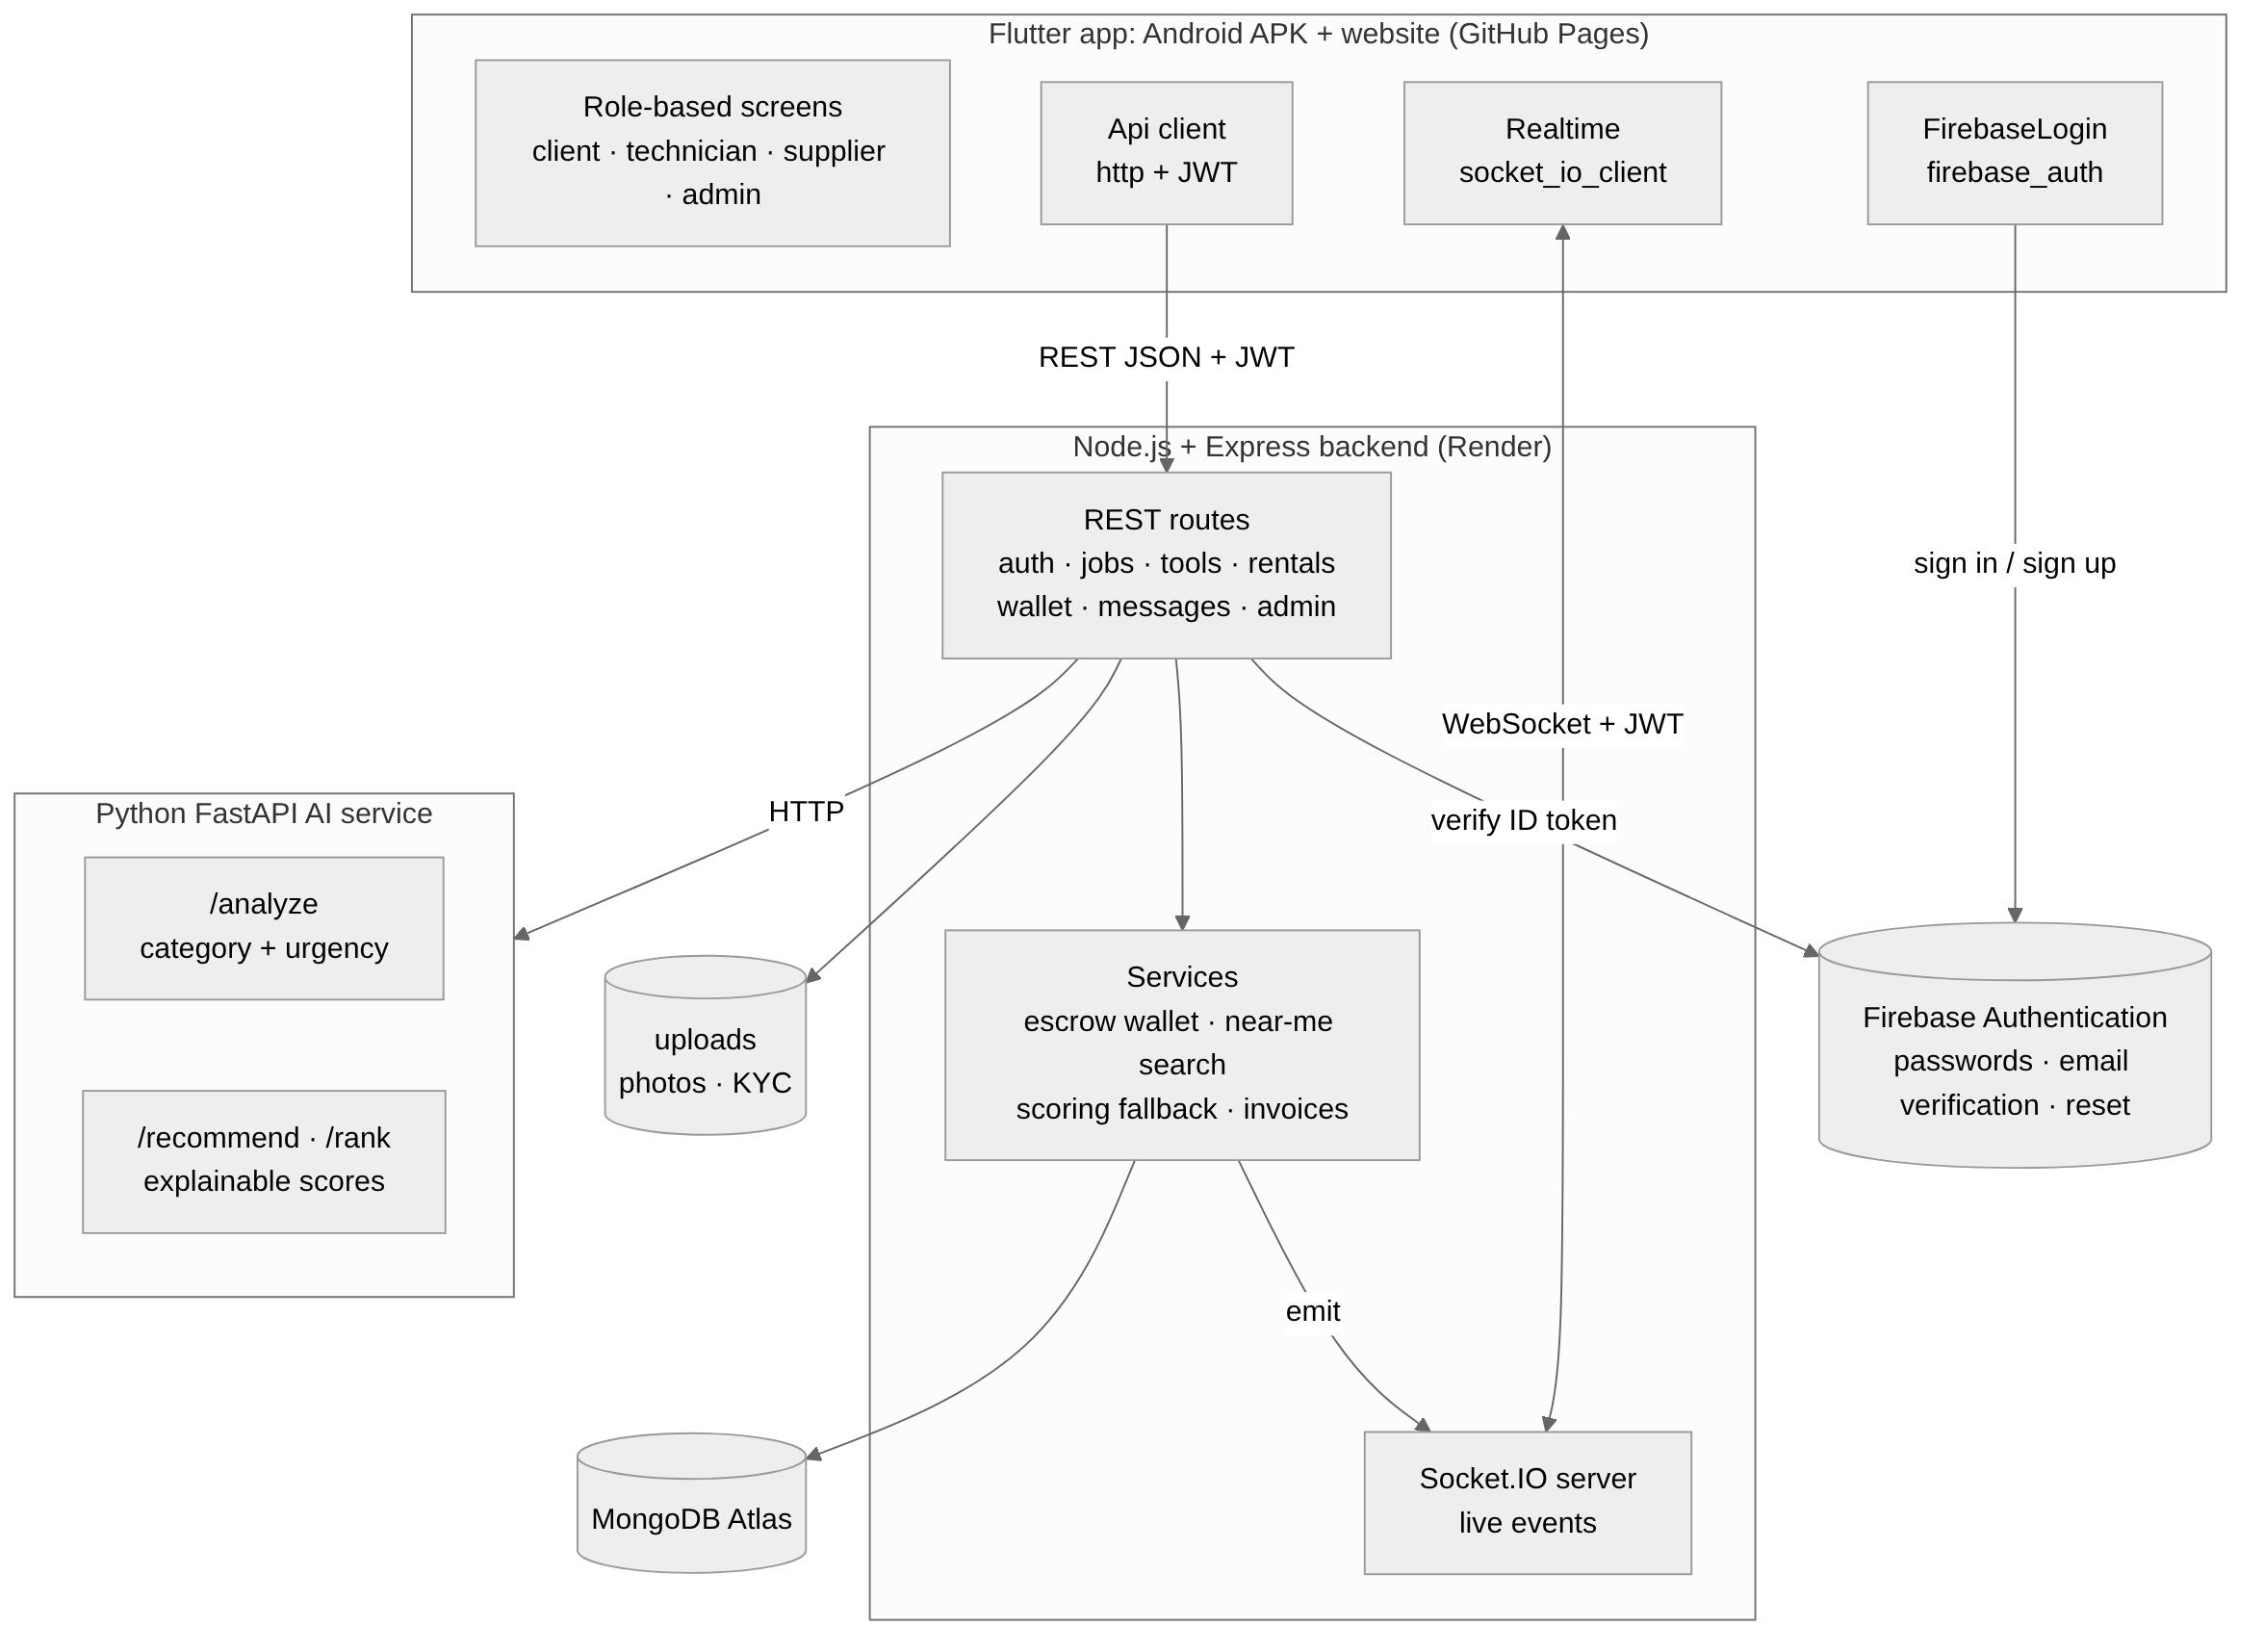
\includegraphics[width=1\linewidth]{Architecture.PNG}
    \caption{Architectural Design}
    \label{fig:placeholder}
\end{figure}

\section{Design Models}
The SureFix system design is illustrated using UML models. The Use Case Diagram shows interactions between users (clients, technicians, suppliers, and admin) and system features like job posting, bidding, the wallet, tool rental and purchase, and KYC. Activity Diagrams explain workflows such as job processing and bidding. The Class Diagram defines system entities and their relationships, while Sequence Diagrams show interactions over time. Together, these models provide a clear view of the system’s structure and behavior.

\newpage


\subsection{Activity Diagram}
This compact activity diagram shows the main system flow based on user roles. After signing up and confirming their email, clients post jobs, hire from AI-ranked quotes with the wallet (escrow) or cash, and confirm completion, which releases the payment; they can also rent or buy tools. Technicians find nearby jobs and send quotes, suppliers list tools and approve requests, and the admin verifies KYC (optional, adding a verified seal) and reviews payments.





\begin{figure}[H]
    \centering
    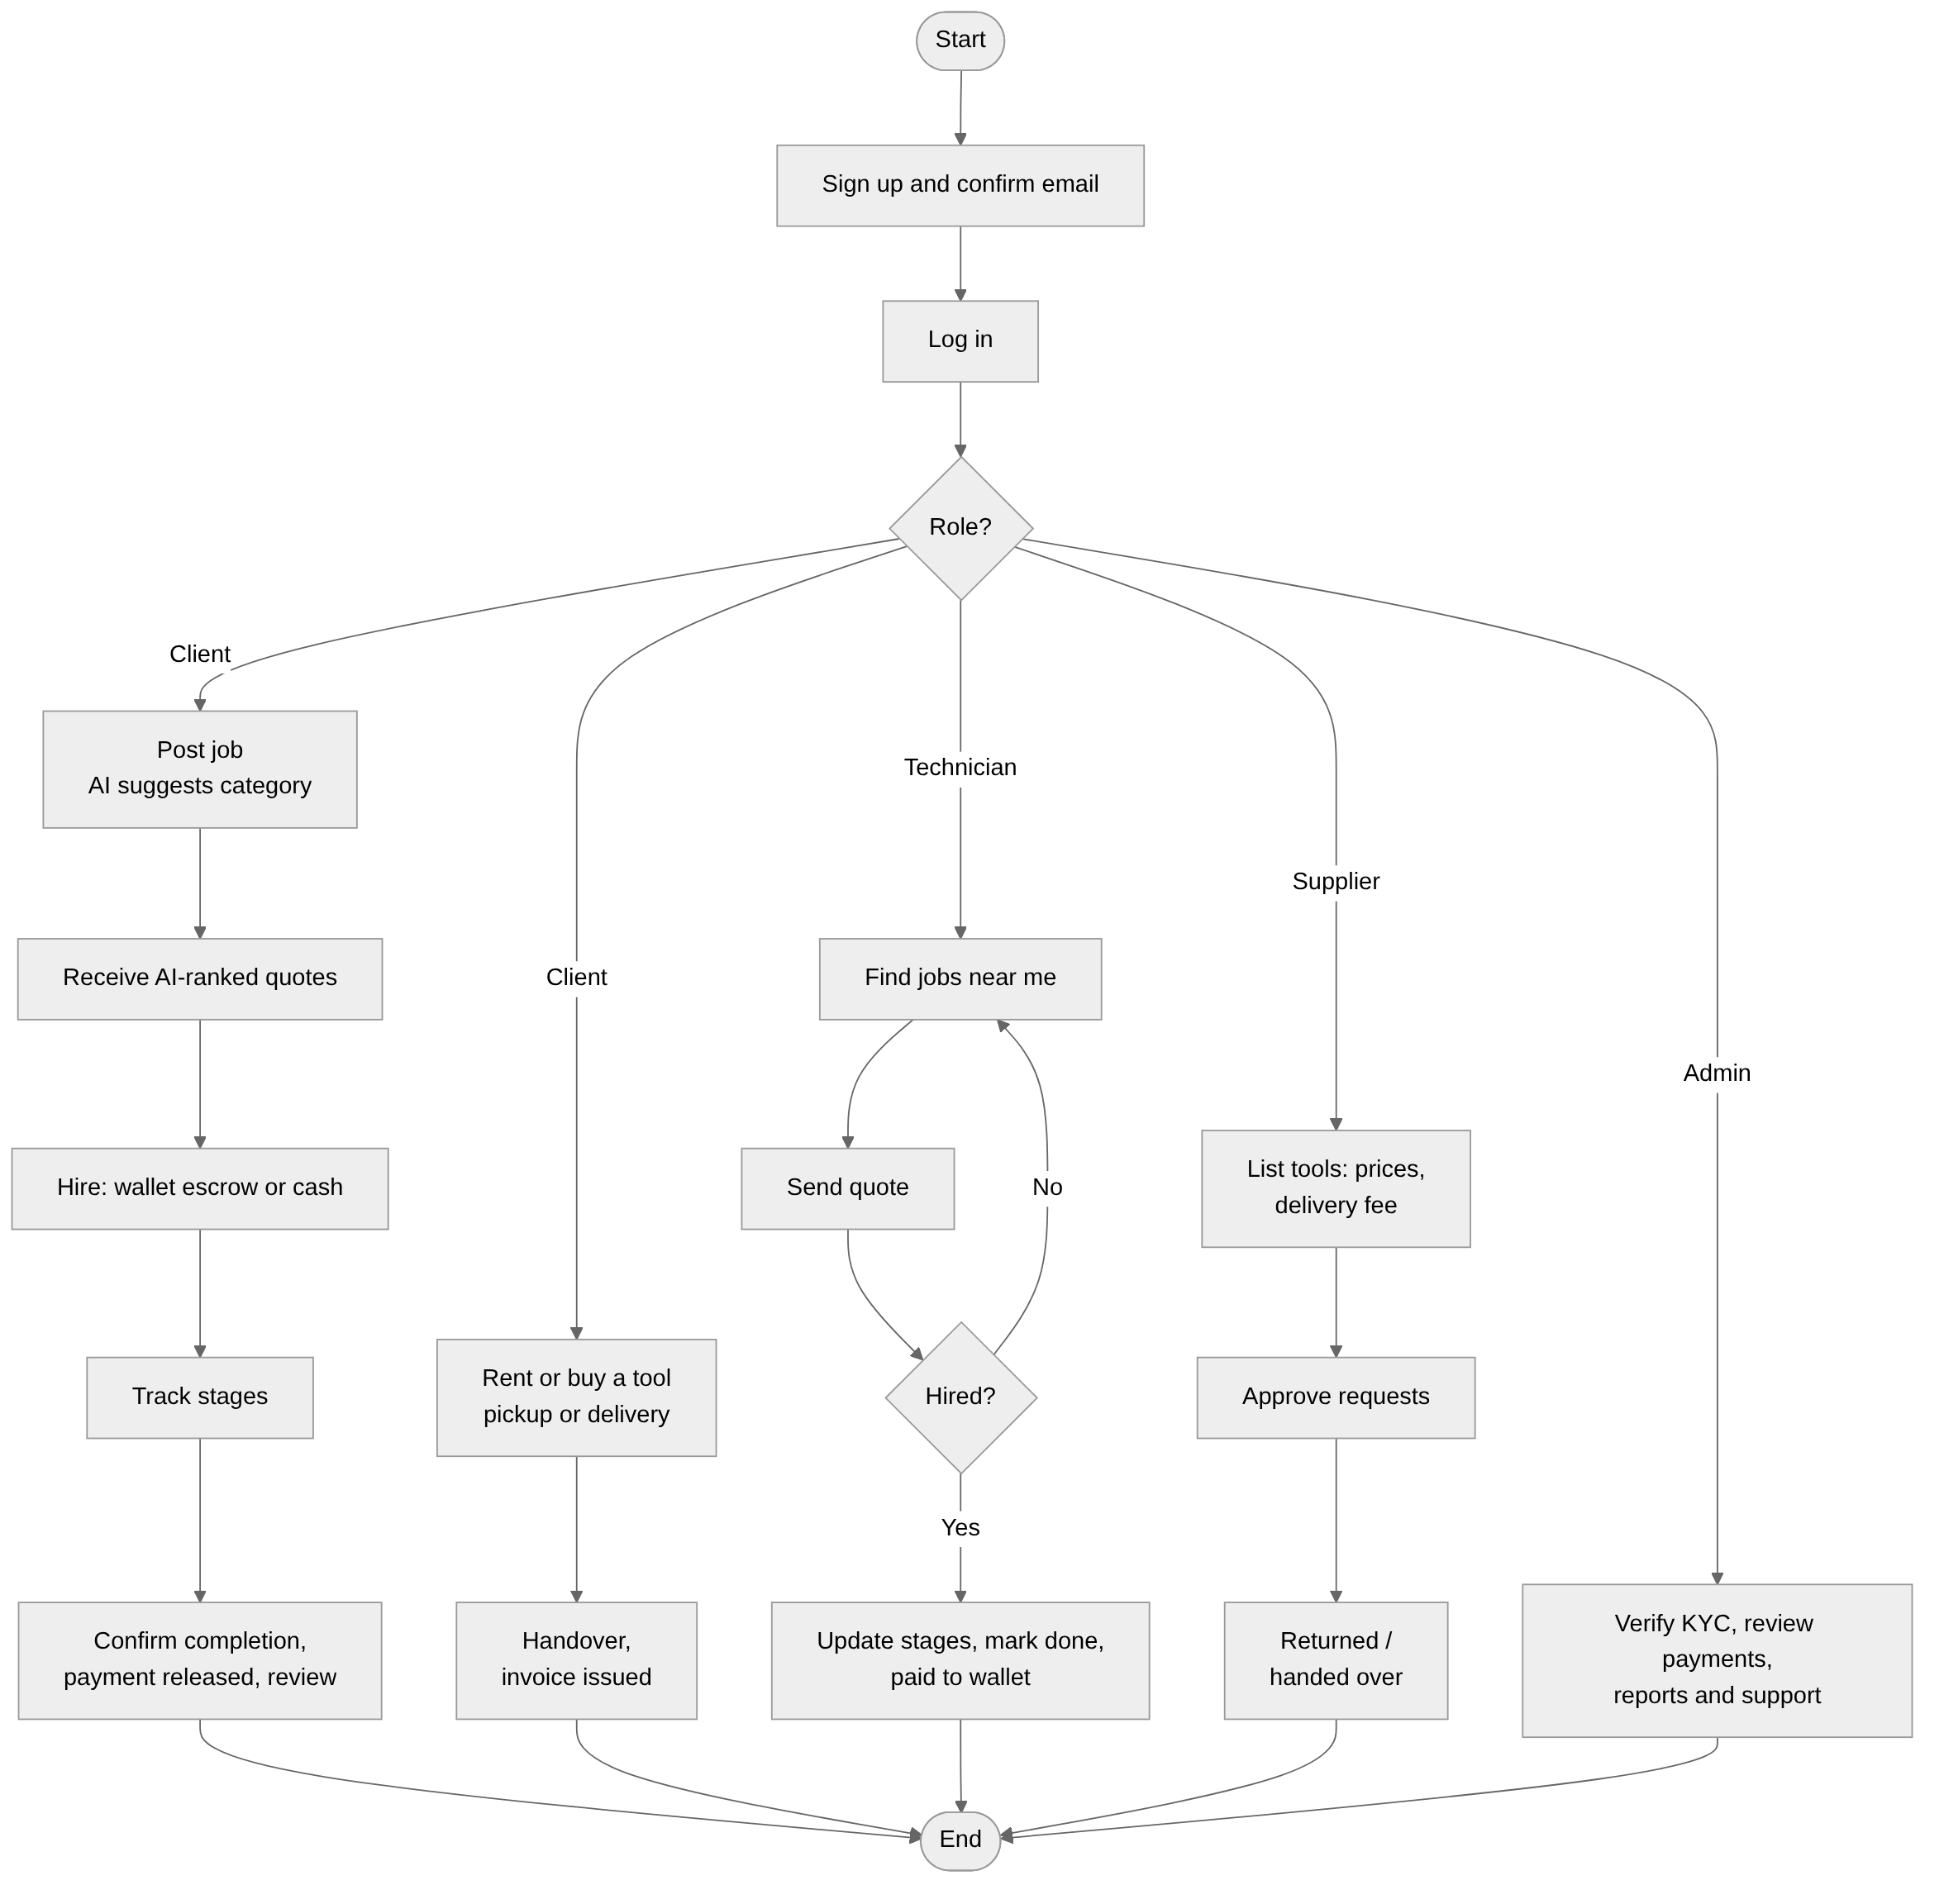
\includegraphics[width=0.85\linewidth]{Compact.png}
    \caption{Activity Diagram – System Workflow (Compact)}

    \label{fig:placeholder}
\end{figure}


\subsection{Usecase Diagram}
The use case diagram represents the interactions between different actors in the SureFix system. Clients can post jobs, use Smart Match, find technicians near them, hire from AI-ranked quotes, confirm completion, rent or buy tools and use the wallet. Technicians find jobs, send quotes and update job stages; suppliers list tools and approve rentals and sales; both can submit KYC. The admin verifies KYC, reviews deposits and withdrawals, manages company accounts and handles support. The diagram also shows dependencies between use cases, such as login, email verification and the wallet.

\begin{figure}[H]
    \centering
    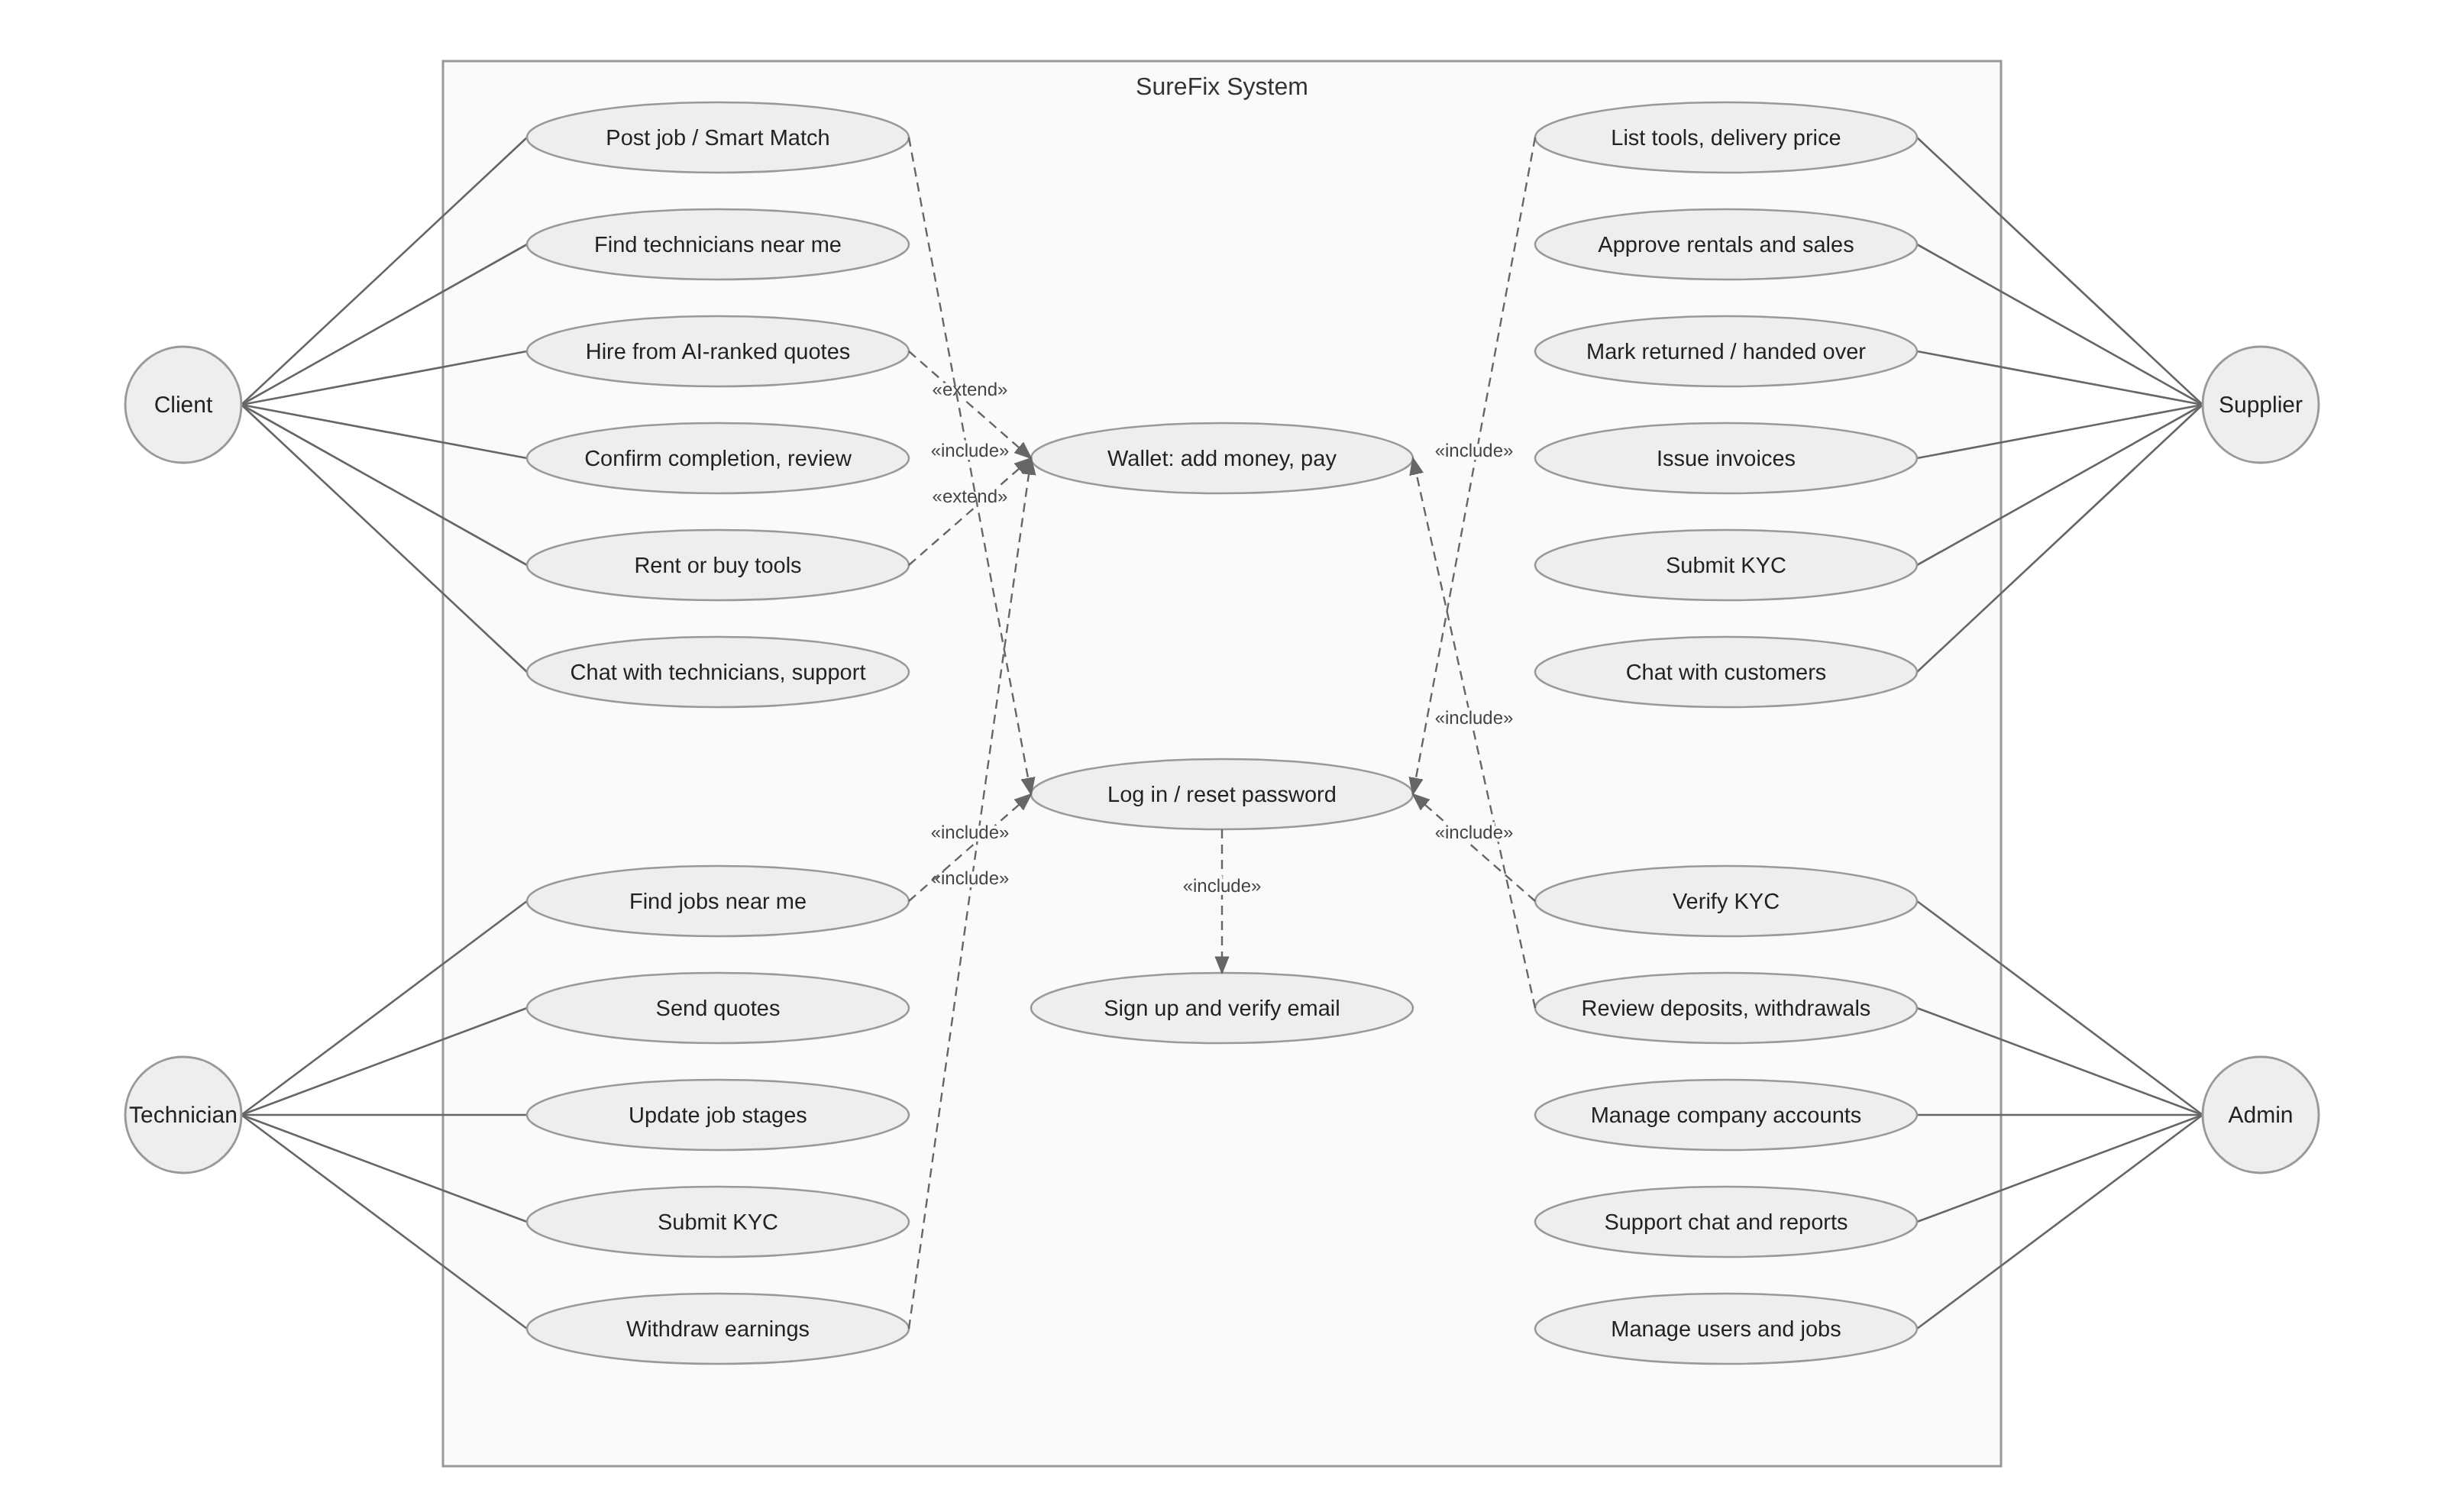
\includegraphics[width=0.95\linewidth]{mermaid-diagram.png}
    \caption{Use Case Diagram}

    \label{fig:placeholder}
\end{figure}


\subsection{Class Diagram}
This class diagram shows all main components of the system, including users, jobs, bids, embedded payments, tools, rentals and purchases, wallet transactions and requests, company payment accounts, messages, notifications, KYC, reports and the AI ranker. It illustrates how users post jobs, place bids, rent or buy tools, move money and communicate.

\begin{figure}[h]
    \centering
    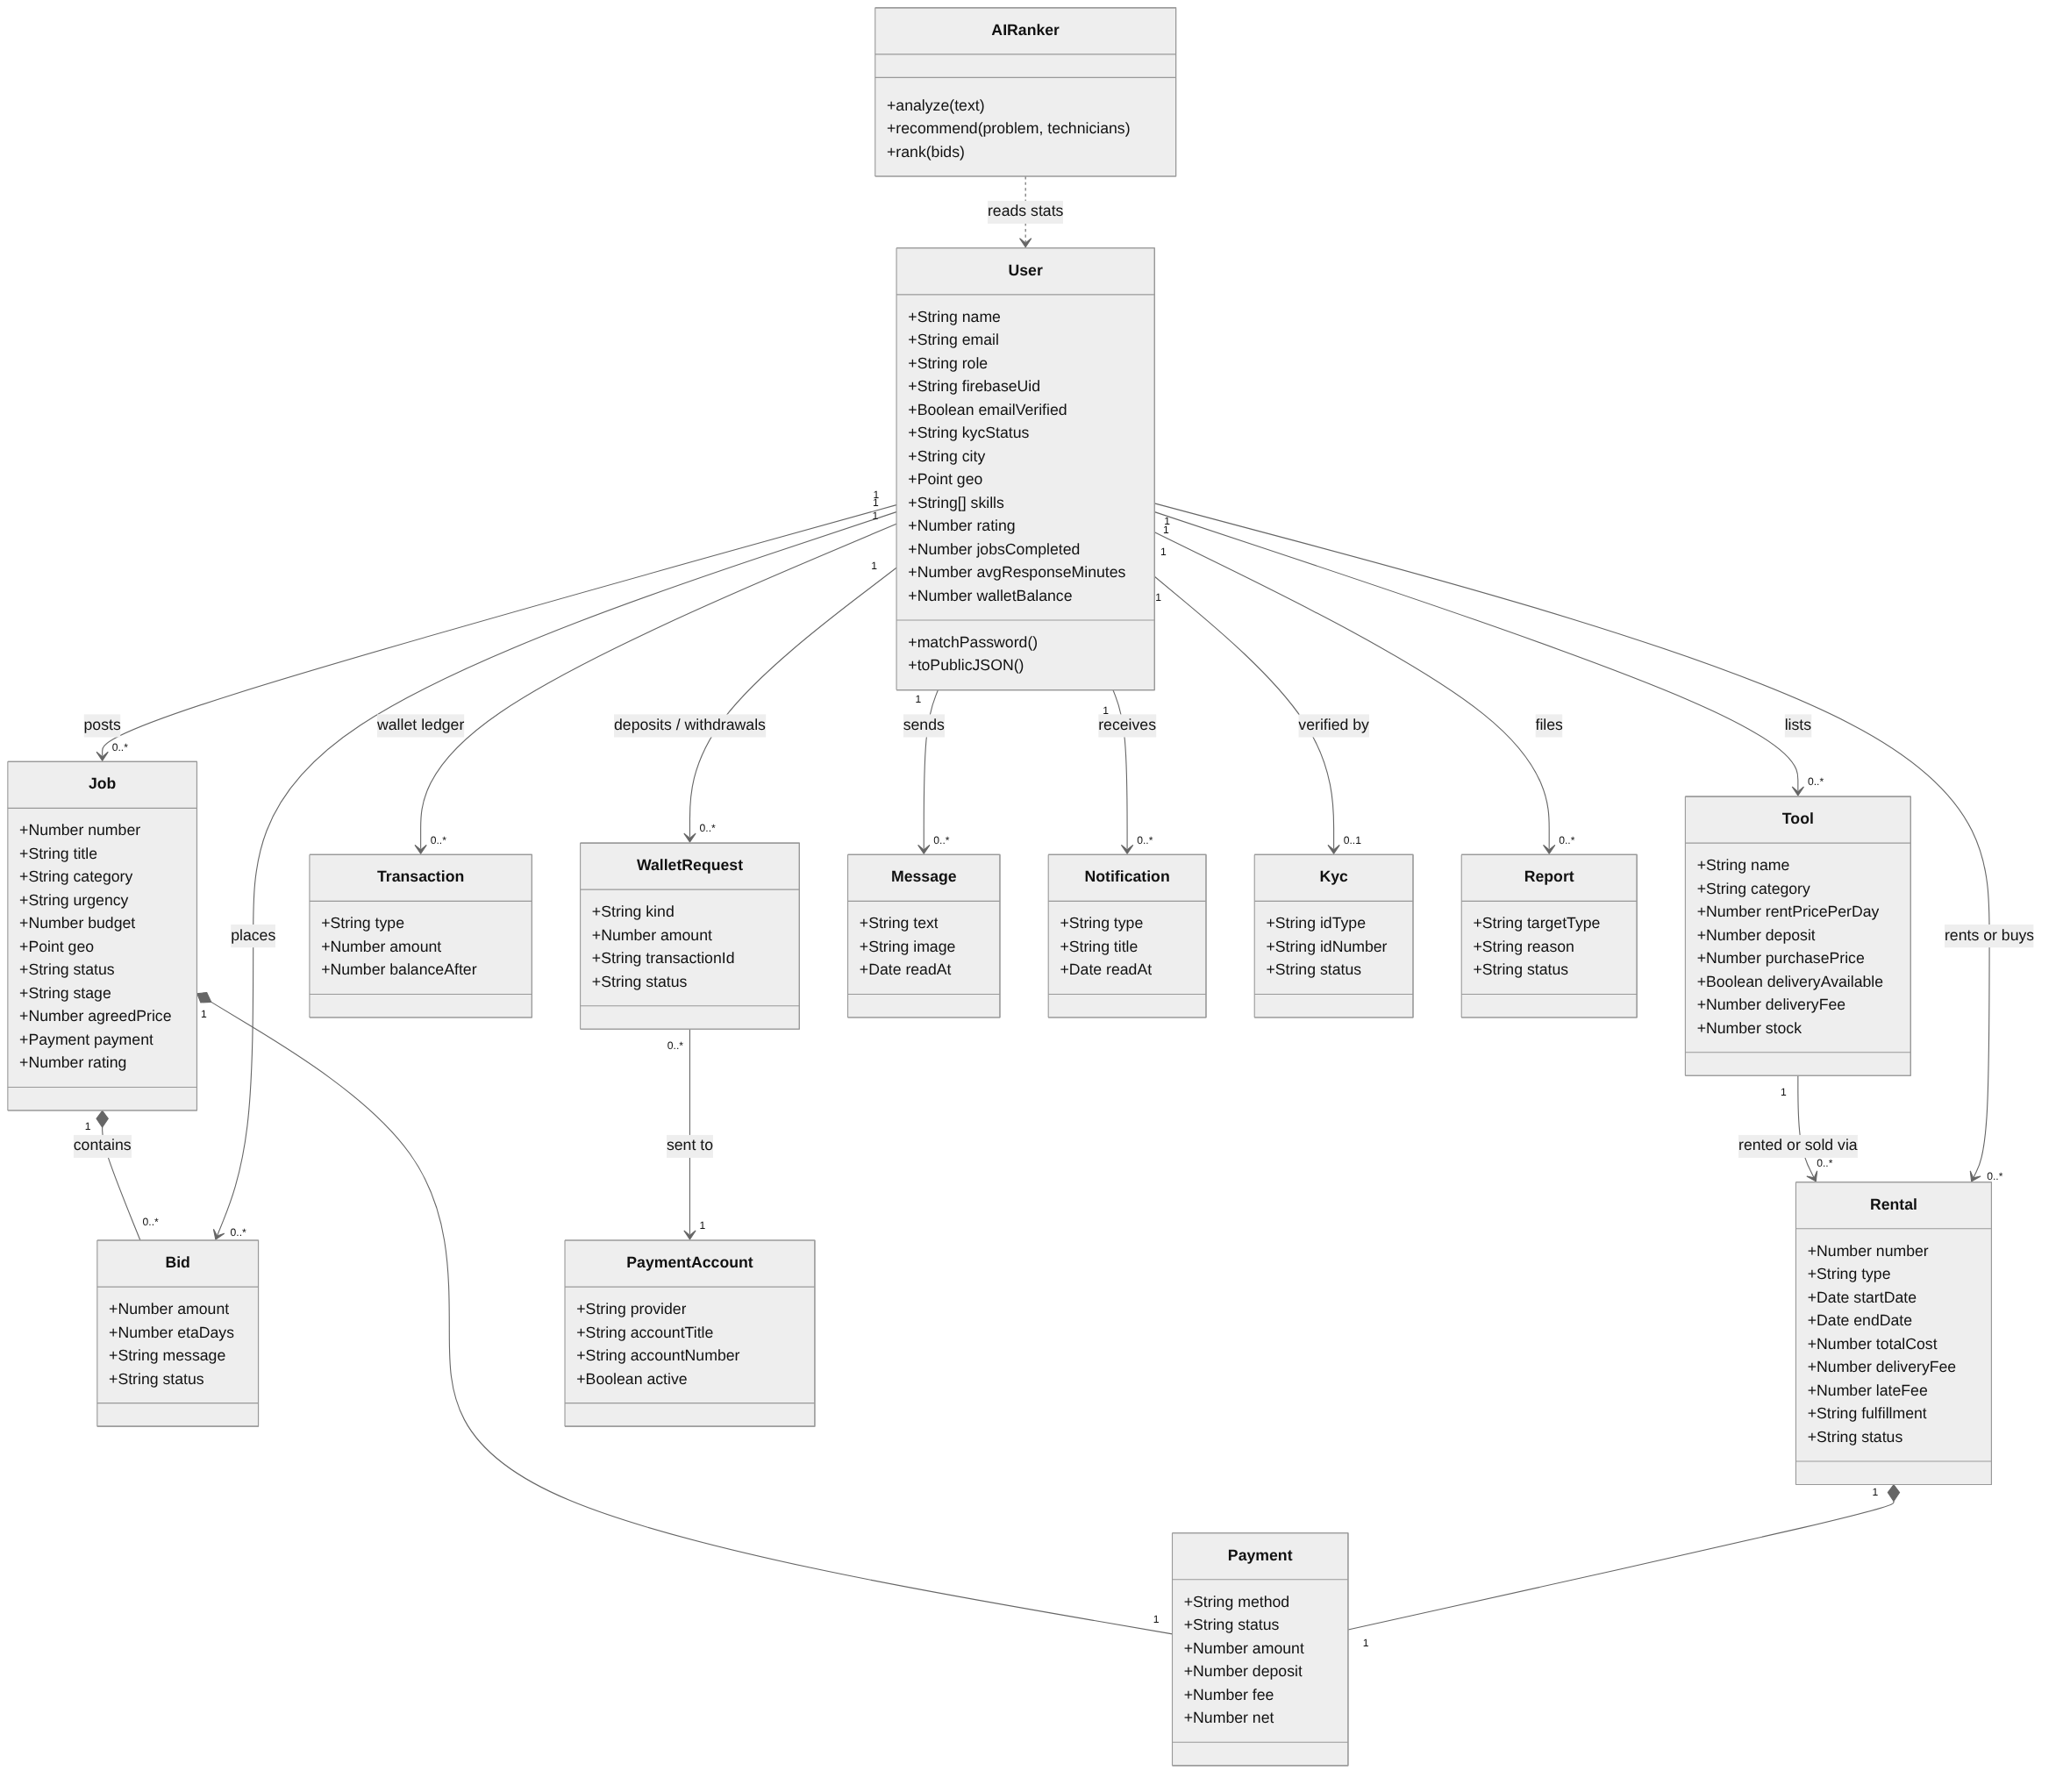
\includegraphics[width=0.95\linewidth]{image1.png}
    \caption{Class Diagram}
    \label{fig:enter-label}
\end{figure}
\subsection{Sequence Diagram}
This sequence diagram illustrates the interaction between different components of the system during the service workflow. It begins when a client posts a job: the backend asks the AI service for the category and urgency, stores the job with its number, and notifies nearby technicians in real time. Technicians then submit quotes, which the AI service ranks with a score, match percentage and reasons before they are shown to the client. The client hires a technician and pays into escrow. The technician reports the stages (on the way, working, done), the client confirms completion, and the payment, minus the 10\% fee, is released to the technician's wallet, after which the client provides feedback.

Overall, it shows how data flows between the application, backend, AI service, database, and the different actors throughout the process.


\begin{figure}[h]
    \centering
    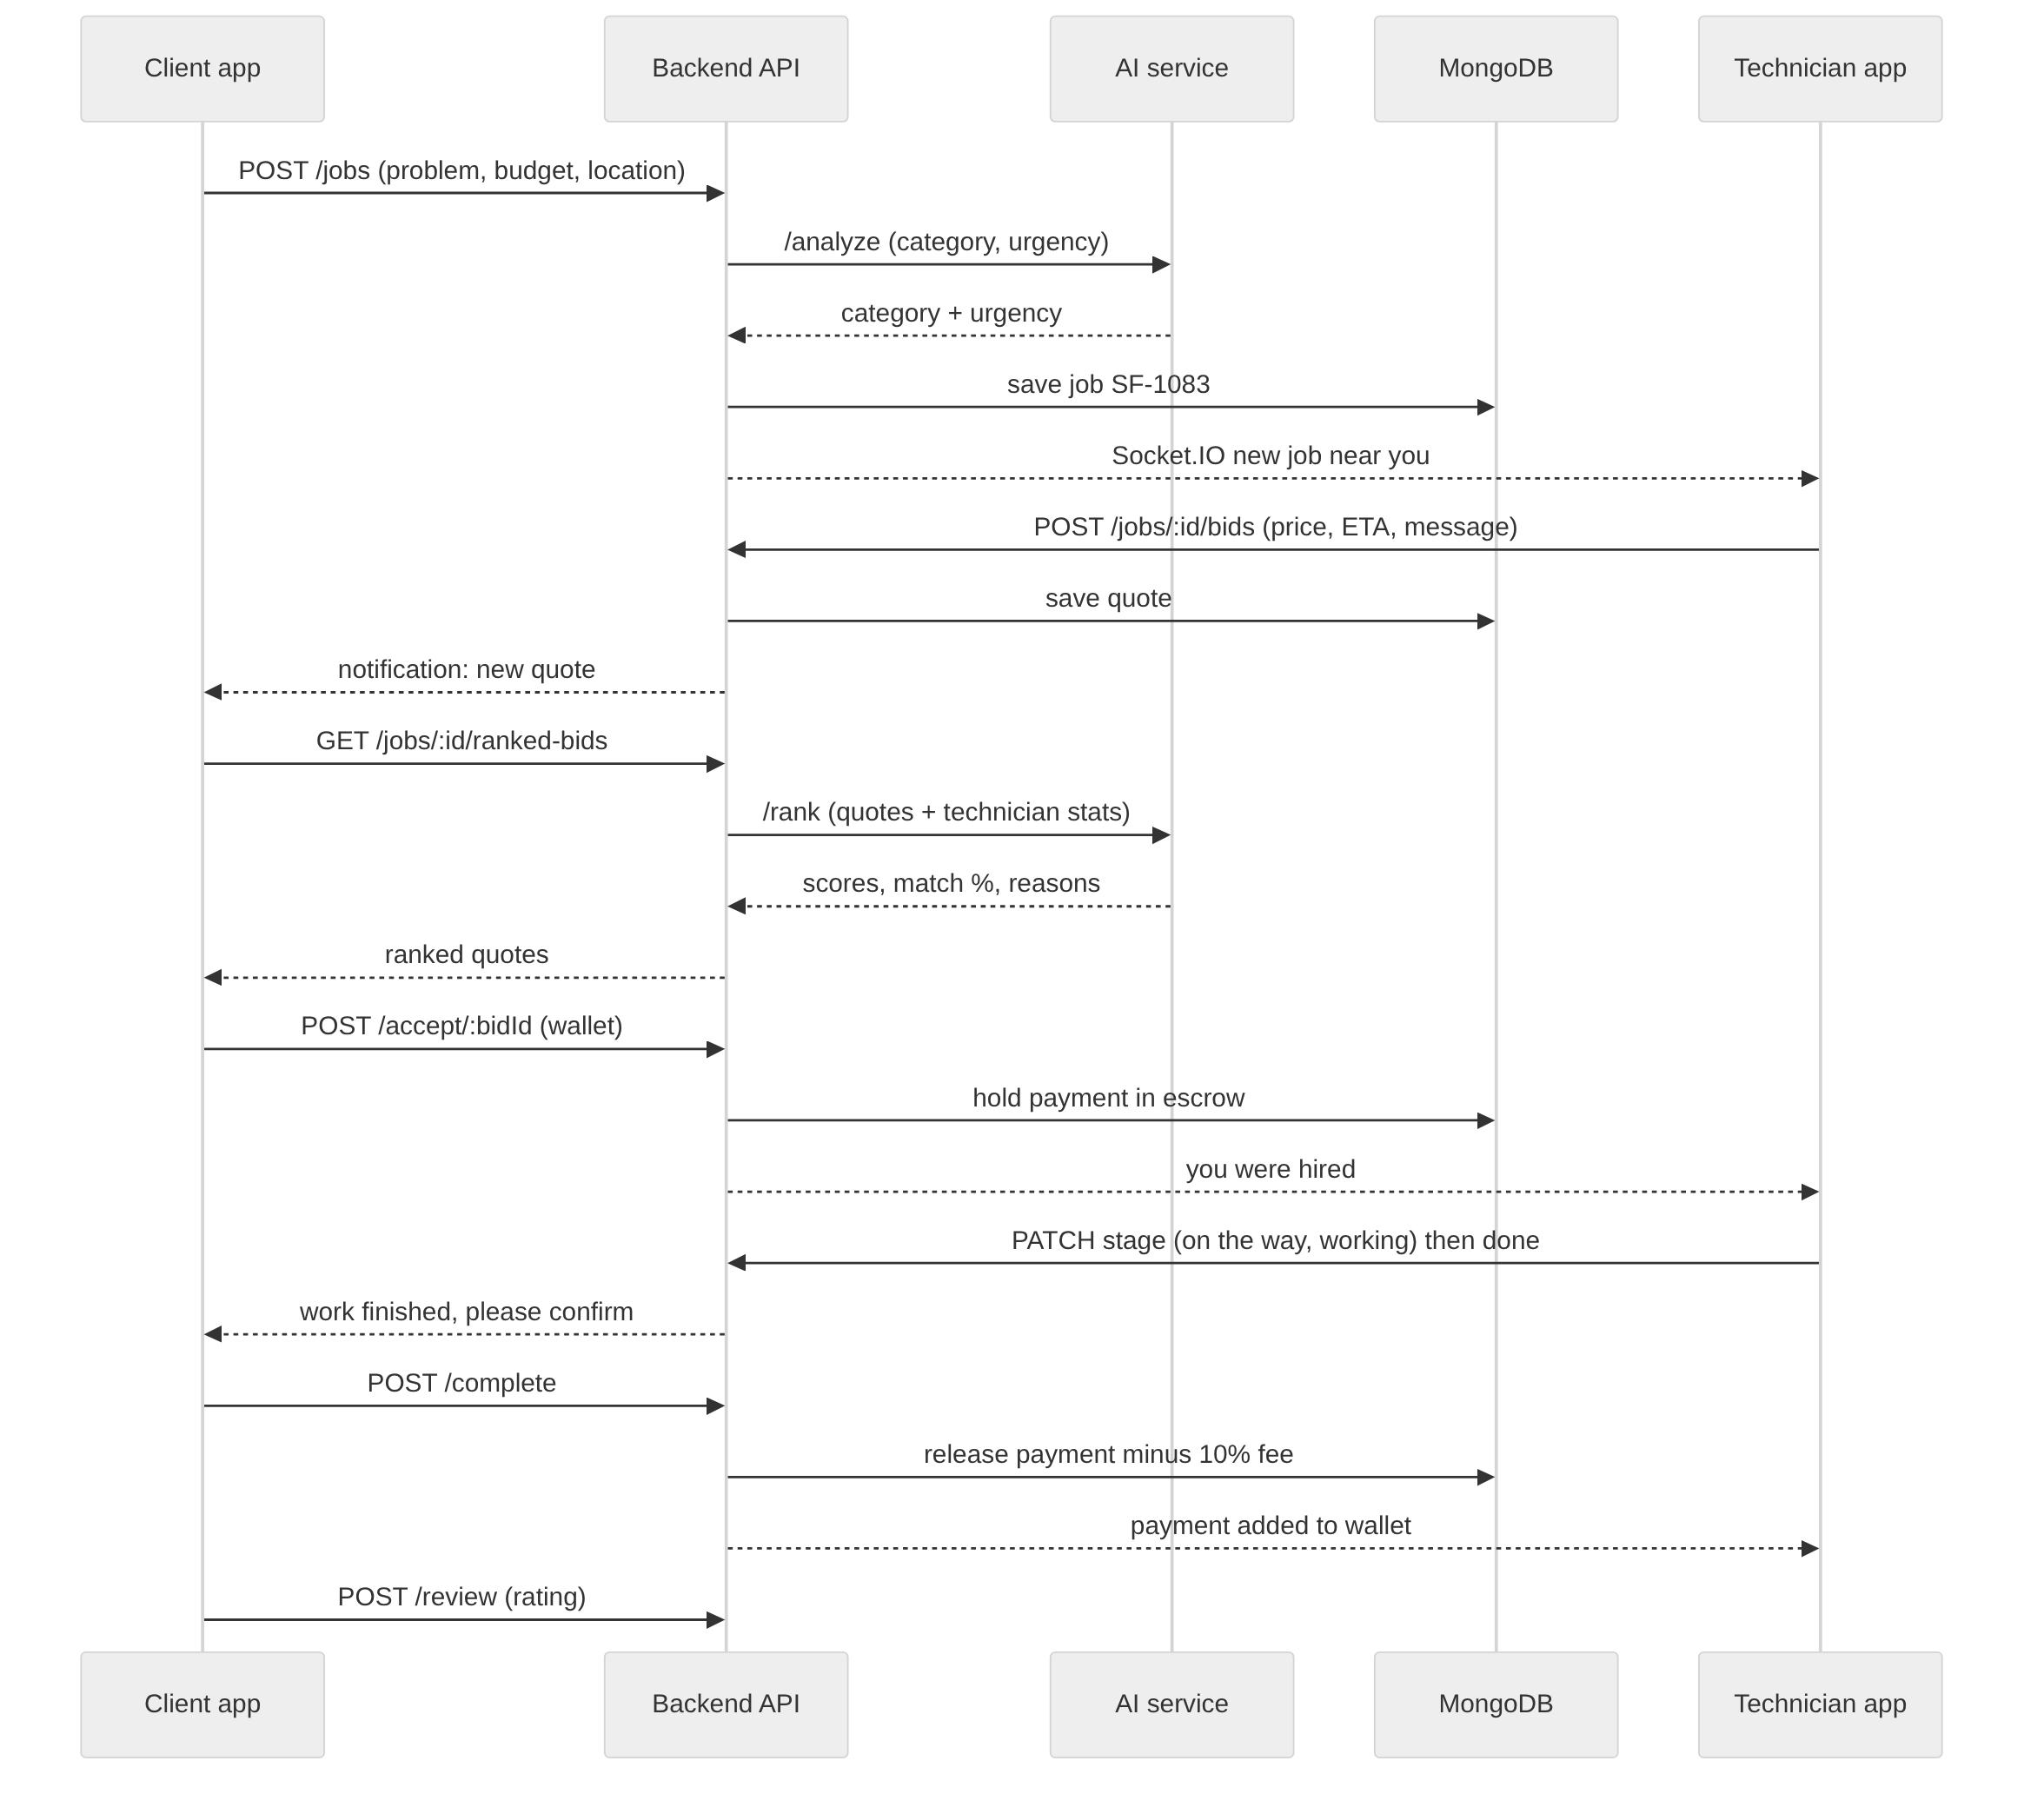
\includegraphics[width=0.95\linewidth]{mermaid-diagram (6).png}
    \caption{Sequence Diagram}
    \label{fig:enter-label}
\end{figure}

\newpage

\subsection{State Transition Diagram }
This state transition diagram shows the two main life cycles of the system. A job is pending while quotes arrive, moves to in progress when the client hires (with its stages hired, on the way, working and done), and becomes completed when the client confirms or 72 hours pass, followed by client feedback; a pending job can be cancelled. A tool request is approved or declined by the supplier; an approved rental ends when it is returned, and an approved purchase ends when it is handed over.


\begin{figure}[H]
    \centering
    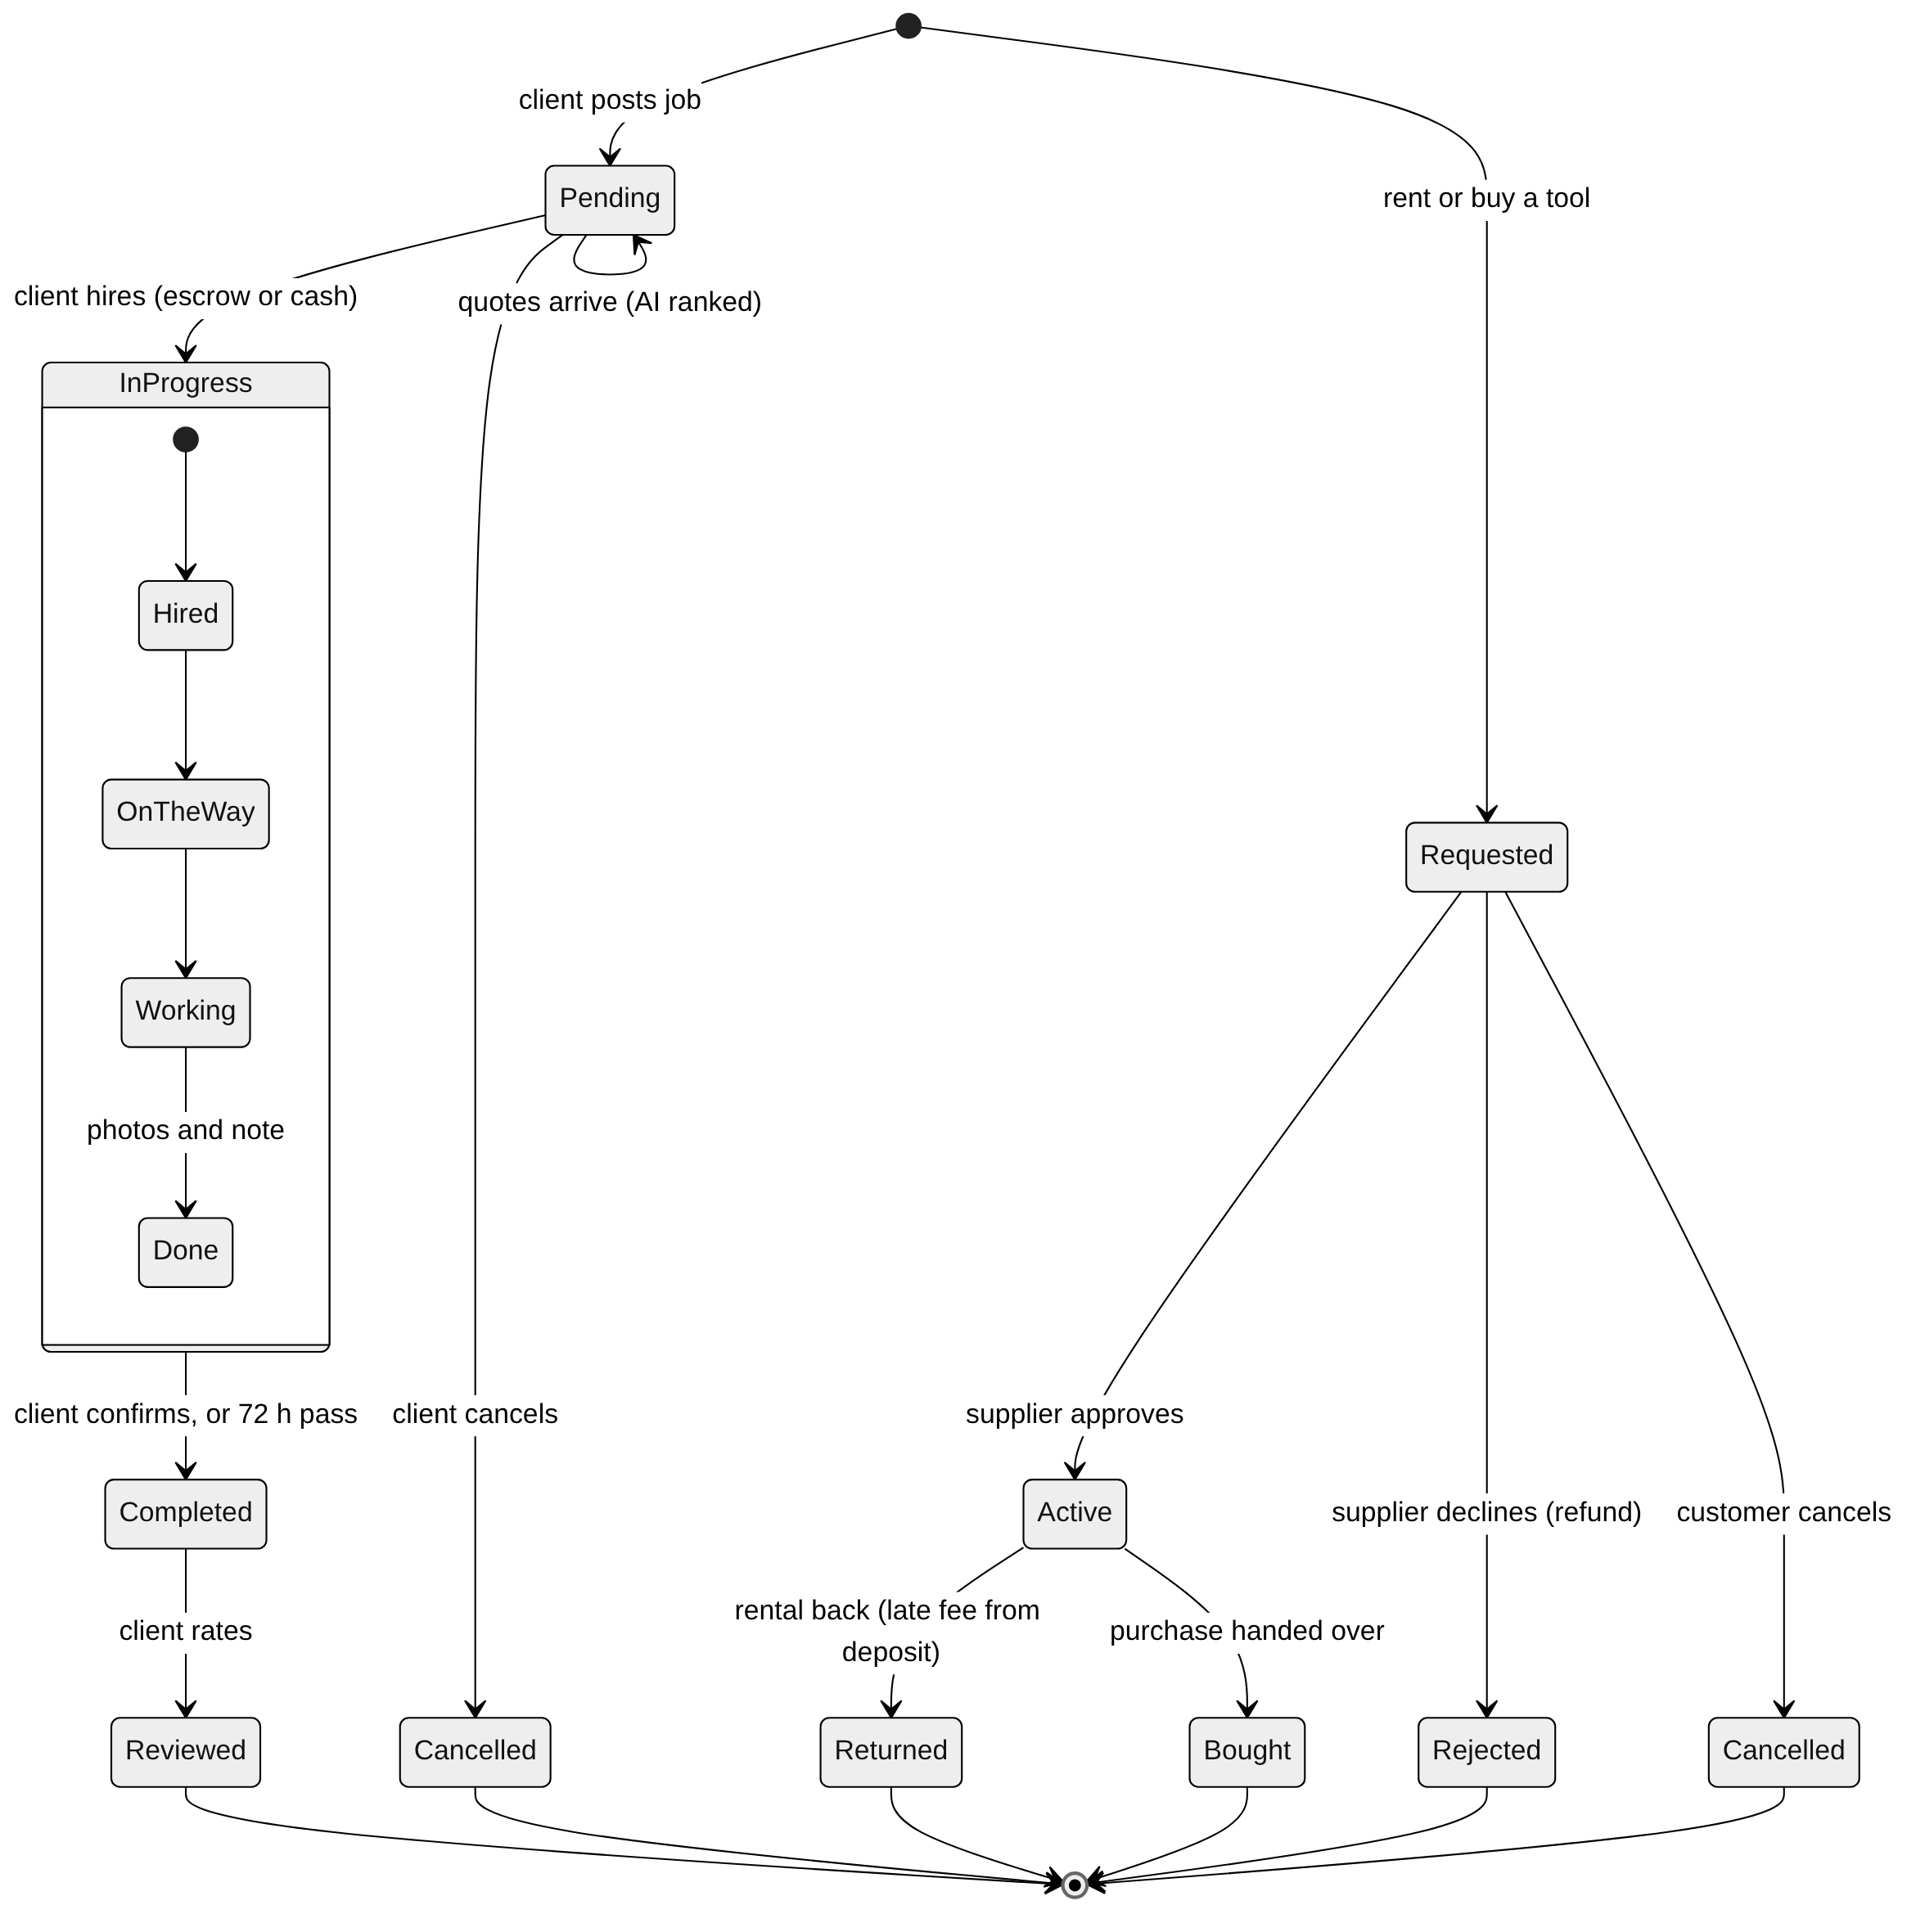
\includegraphics[width=0.63\linewidth]{mermaid-diagram (8).png}
    \caption{State Transition Diagram}
    \label{fig:enter-label}
\end{figure}


\section{Data Design}

The system’s information domain begins with user-generated inputs such as job details, bids, tool listings, and messages. Unlike real-time processing systems, this platform uses persistent storage to manage and maintain all data. The core data transformation is as follows:

\begin{enumerate}
    \item \textbf{User Input Data:}  
    Data is entered by users through the application, including registration details, job postings, bids, tool information, wallet requests and messages. This data is transmitted to the backend via REST API requests in JSON format.

    \item \textbf{API Processing:}  
        The backend server (Node.js) receives the requests, validates the input data, and processes it based on business logic. Authentication is handled with Firebase ID tokens exchanged for JWT sessions to ensure secure access.

    \item \textbf{Database Storage:}  
    The processed data is stored in MongoDB using structured collections. Key entities include:
    \begin{itemize}
        \item \textbf{User:} Stores user details such as role, profile, KYC status, and ratings.
        \item \textbf{Job:} Contains job information such as title, description, status, and assigned technician.
        \item \textbf{Bid:} Stores technician bids linked to jobs.
        \item \textbf{Tool:} Contains tool details listed by suppliers.
                \item \textbf{Rental:} Stores rentals and one-time purchases with delivery fee, late fee, invoice number and payment.
        \item \textbf{Transaction:} Stores every wallet movement (holds, releases, refunds, fees, deposits, withdrawals) with the balance after it.
        \item \textbf{WalletRequest / PaymentAccount:} Store deposit and withdrawal requests and the company accounts they use.
        \item \textbf{Message:} Stores communication between users and with SureFix Support.
        \item \textbf{Notification:} Stores system-generated alerts and updates.
    \end{itemize}

    \item \textbf{AI Data Processing:}  
    Relevant technician data (ratings, job completion rate, response time, and skills) is sent to the AI service. The service processes this data and returns a ranking score for each technician.

    \item \textbf{Output Data:}  
    The final processed data, such as job details, ranked bids, notifications, and messages, is returned to the mobile application in JSON format for display.
\end{enumerate}

\textbf{Data Storage Items}

\begin{itemize}
    \item \textbf{User Data:} Stored in MongoDB collections with role-based attributes.
    \item \textbf{Job and Bid Data:} Maintained with relationships between clients and technicians.
        \item \textbf{Tool and Rental Data:} Stored for supplier inventory, rentals, sales and invoices.
    \item \textbf{Wallet Data:} Balances, ledger transactions and deposit/withdrawal requests.
    \item \textbf{Messages and Notifications:} Stored for communication and real-time updates.
    \item \textbf{AI Output Data:} Ranking scores are generated dynamically and returned via API.
\end{itemize}


\subsection{Data Dictionary}

This section presents a structured list of key data entities used in the SureFix system along with their types and descriptions. It helps in understanding how data is organized, stored, and managed within the application.
\begin{longtable}{|p{0.3\textwidth}|p{0.25\textwidth}|p{0.35\textwidth}|}
\caption{Data Dictionary of System Entities} \\

\hline
\textbf{Entity (Variable)} & \textbf{Type} & \textbf{Description} \\ 
\hline
\endfirsthead

\hline
\textbf{Entity (Variable)} & \textbf{Type} & \textbf{Description} \\ 
\hline
\endhead

User & Object (JSON) & Stores user information such as name, email, role, KYC status, and profile details. \\ \hline

Job & Object (JSON) & Represents a service request posted by a client. \\ \hline

Bid & Object (JSON) & Contains technician bid details such as amount and ETA. \\ \hline

Tool & Object (JSON) & Stores tool information listed by suppliers. \\ \hline

Rental & Object (JSON) & Represents a tool rental or one-time purchase, with its invoice. \\ \hline

Transaction & Object (JSON) & One wallet movement and the balance after it. \\ \hline

WalletRequest & Object (JSON) & A deposit or withdrawal waiting for admin review. \\ \hline

PaymentAccount & Object (JSON) & A company bank or mobile-wallet account. \\ \hline

Report & Object (JSON) & A user's report about a person, job or tool. \\ \hline

Message & Object (JSON) & Stores communication data between users. \\ \hline

Notification & Object (JSON) & Represents system-generated alerts. \\ \hline

KYC & Object (JSON) & Stores verification details for technicians and suppliers. \\ \hline

Rating & Float & Represents technician rating (0–5). \\ \hline

Job Status & String & Indicates job state (pending, in\_progress, completed, cancelled). \\ \hline

Job Number & Integer & Public job reference shown as SF-1001 onwards. \\ \hline

Invoice Number & Integer & Rental or purchase reference shown as INV-1001 onwards. \\ \hline

Geo Point & GeoJSON Point & Saved location, used only to compute distances. \\ \hline

Wallet Balance & Float & Money available in the user's wallet (PKR). \\ \hline

Bid Amount & Float & Proposed price by technician. \\ \hline

JWT Token & String & SureFix session, issued after Firebase sign-in. \\ \hline

AI Score & Float & Ranking score generated by AI. \\ \hline

Timestamp & DateTime & Stores date and time values. \\ \hline

\end{longtable}

\section{Human Interface Design}

The system is designed with a clean interface that works on phones and desktop browsers to ensure ease of use for all users, regardless of technical expertise. The application follows a simple, role-based flow, allowing users to perform tasks efficiently through intuitive navigation and clear visual feedback.

\begin{enumerate}

\item \textbf{User Registration and Login}  
\textbf{User Action:} The user begins by creating an account or logging in using email and password. The interface provides a simple form with role selection (client, technician, or supplier), followed by a ``Confirm your email'' step.    

\textbf{Guidance:} Input fields are clearly labeled, and validation messages are shown instantly for incorrect or missing information.

\item \textbf{Navigating the Application}  
\textbf{User Action:} After login, the user is directed to a role-specific home screen. A sidebar (on wide screens) or a bottom dock (on phones) provides access to the user's sections, such as Jobs, Technicians, Tools, Messages, Notifications, Wallet and Account.    

\textbf{Guidance:} Icons and labels are used to make navigation simple and consistent across all screens.

\item \textbf{Performing Core Actions}  
\textbf{User Action:}  
Clients can post jobs, view AI-ranked quotes, hire technicians, pay through the wallet, and rent or purchase tools. Technicians can find jobs near them, send quotes, and update their work. Suppliers can add tools, set prices and delivery, approve requests and issue invoices.    

\textbf{Guidance:} Each action is supported with buttons, forms, and clear instructions. Dropdowns and input fields ensure structured data entry.

\item \textbf{Real-Time Feedback and Communication}  
\textbf{Feedback:} The system provides instant feedback using snackbars (toast messages) for every action, such as ``Job posted successfully'' or ``Bid submitted.'' Users also receive real-time notifications and messages that update automatically.

\item \textbf{Job and Task Completion}  
\textbf{User Action:} Users can track job status (Pending $\rightarrow$ In Progress: hired, on the way, working, done $\rightarrow$ Completed) and perform actions like confirming completion, which releases the payment, or submitting ratings.    

\textbf{Feedback:} Confirmation messages and updated status indicators are displayed immediately.

\item \textbf{Ending the Session}  
\textbf{User Action:} The user can log out from the account menu.    

\textbf{Feedback:} The system securely logs out the user and returns to the login screen.

\end{enumerate}

\subsection{Screen Images} 
The following section presents the user interface of the current SureFix system from the user’s perspective, captured from the website (the Android app shows the same screens in a phone layout). It includes key screens that demonstrate the main functionalities of the application, such as authentication, job management, tool rental and purchase, the wallet, and communication. These interfaces are designed to be simple, intuitive, and user-friendly for all roles.\newline

\textbf{Login Screen}
\begin{figure}[H]
    \centering
    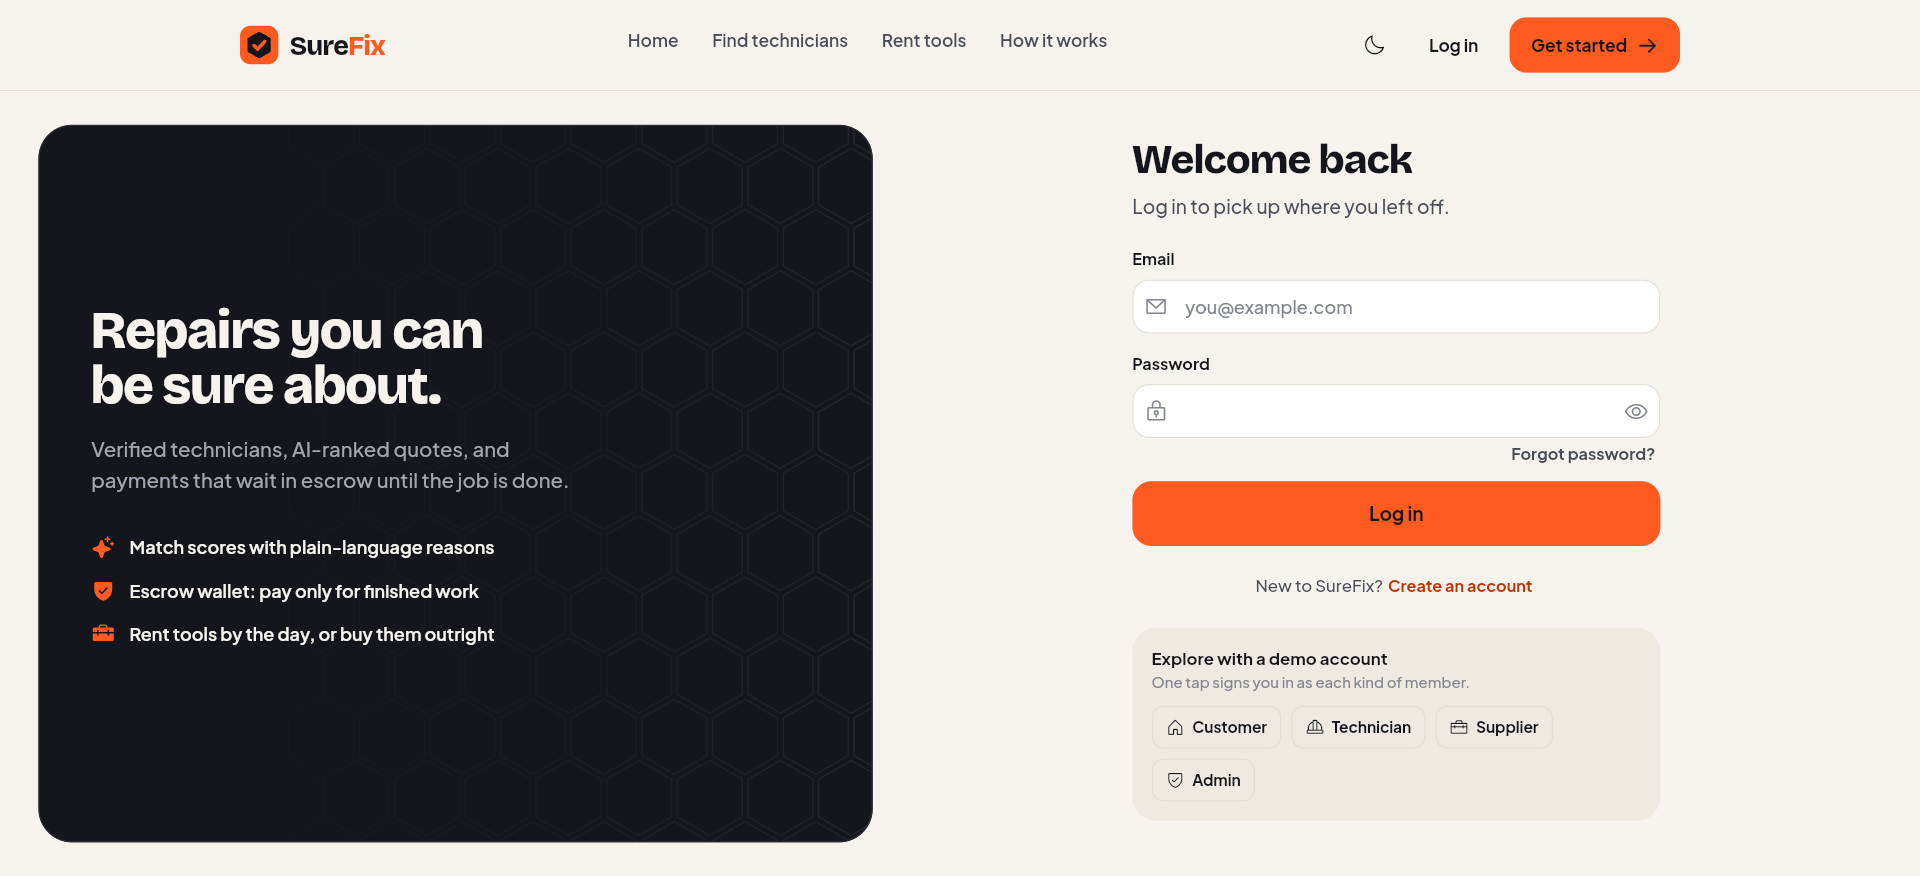
\includegraphics[width=1\linewidth]{login desk.png}
        \caption{This screen allows users to log in using their email and password through Firebase Authentication, with a forgot-password link. After login users are redirected to their role's dashboard.}
    \label{fig:placeholder}
\end{figure}

\textbf{Registration Screen}

\begin{figure}[H]
    \centering
    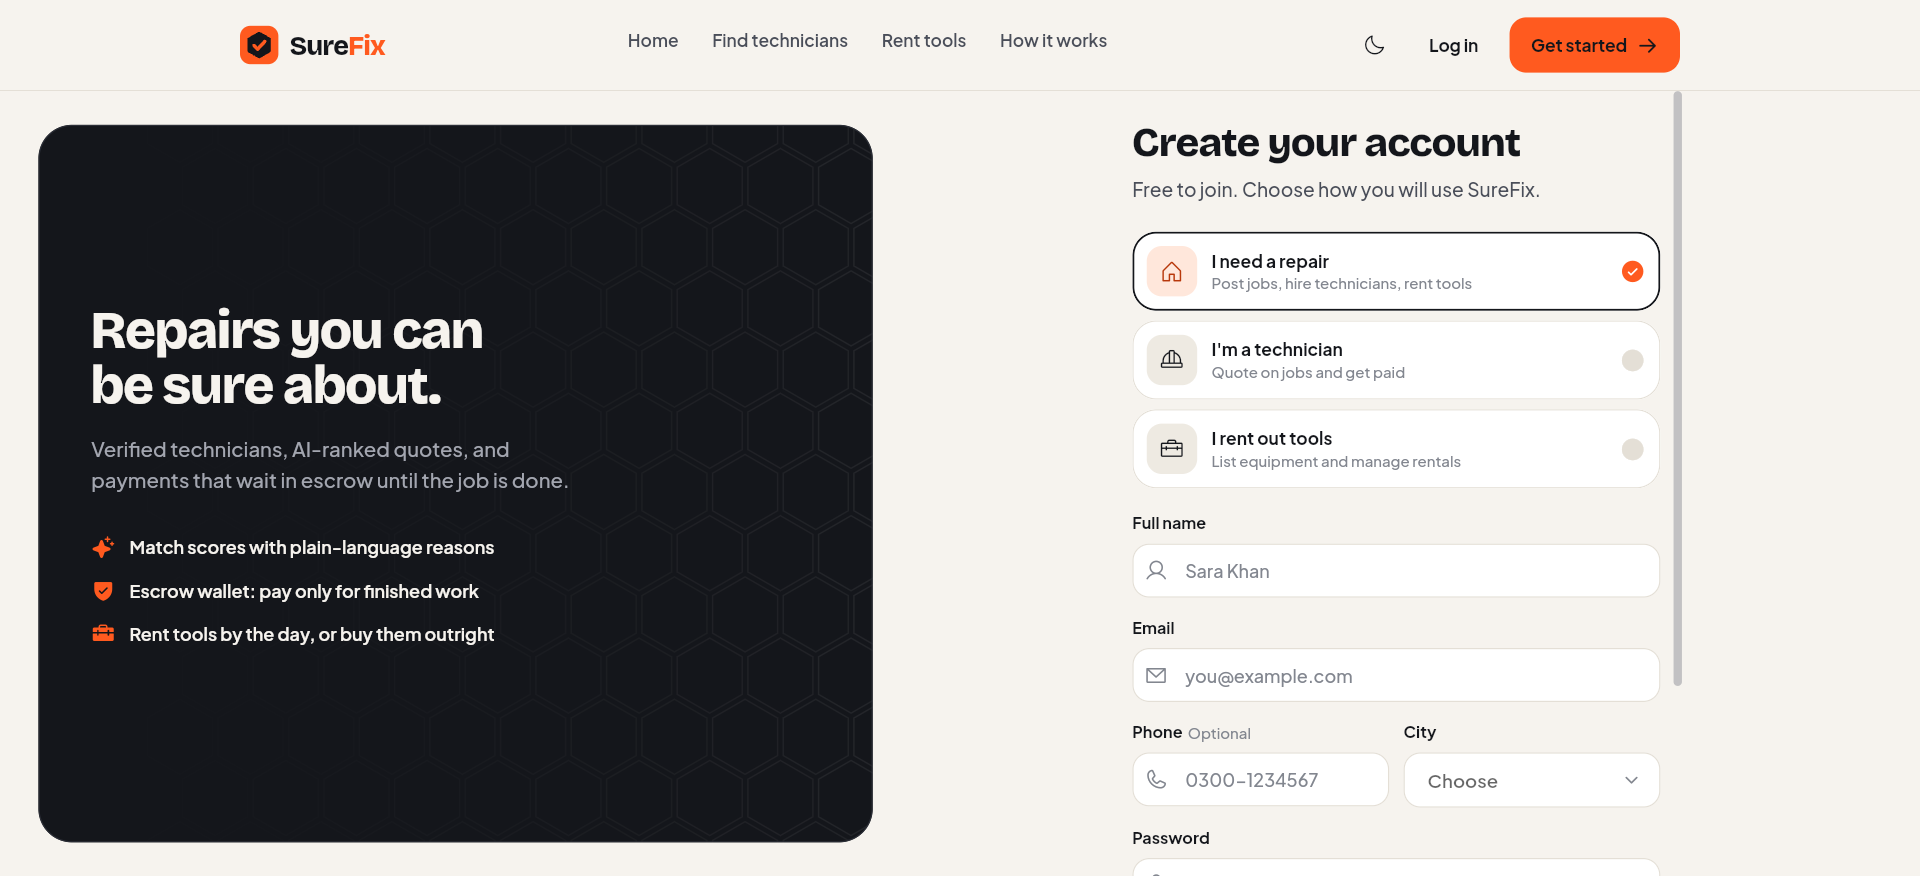
\includegraphics[width=1\linewidth]{register desk.png}
        \caption{This screen enables new users to create an account by choosing a role (client, technician or supplier) and entering their details; the email must then be confirmed.}
    \label{fig:placeholder}
\end{figure}

\newpage
\textbf{Client Dashboard (My Jobs)}

\begin{figure}[H]
    \centering
    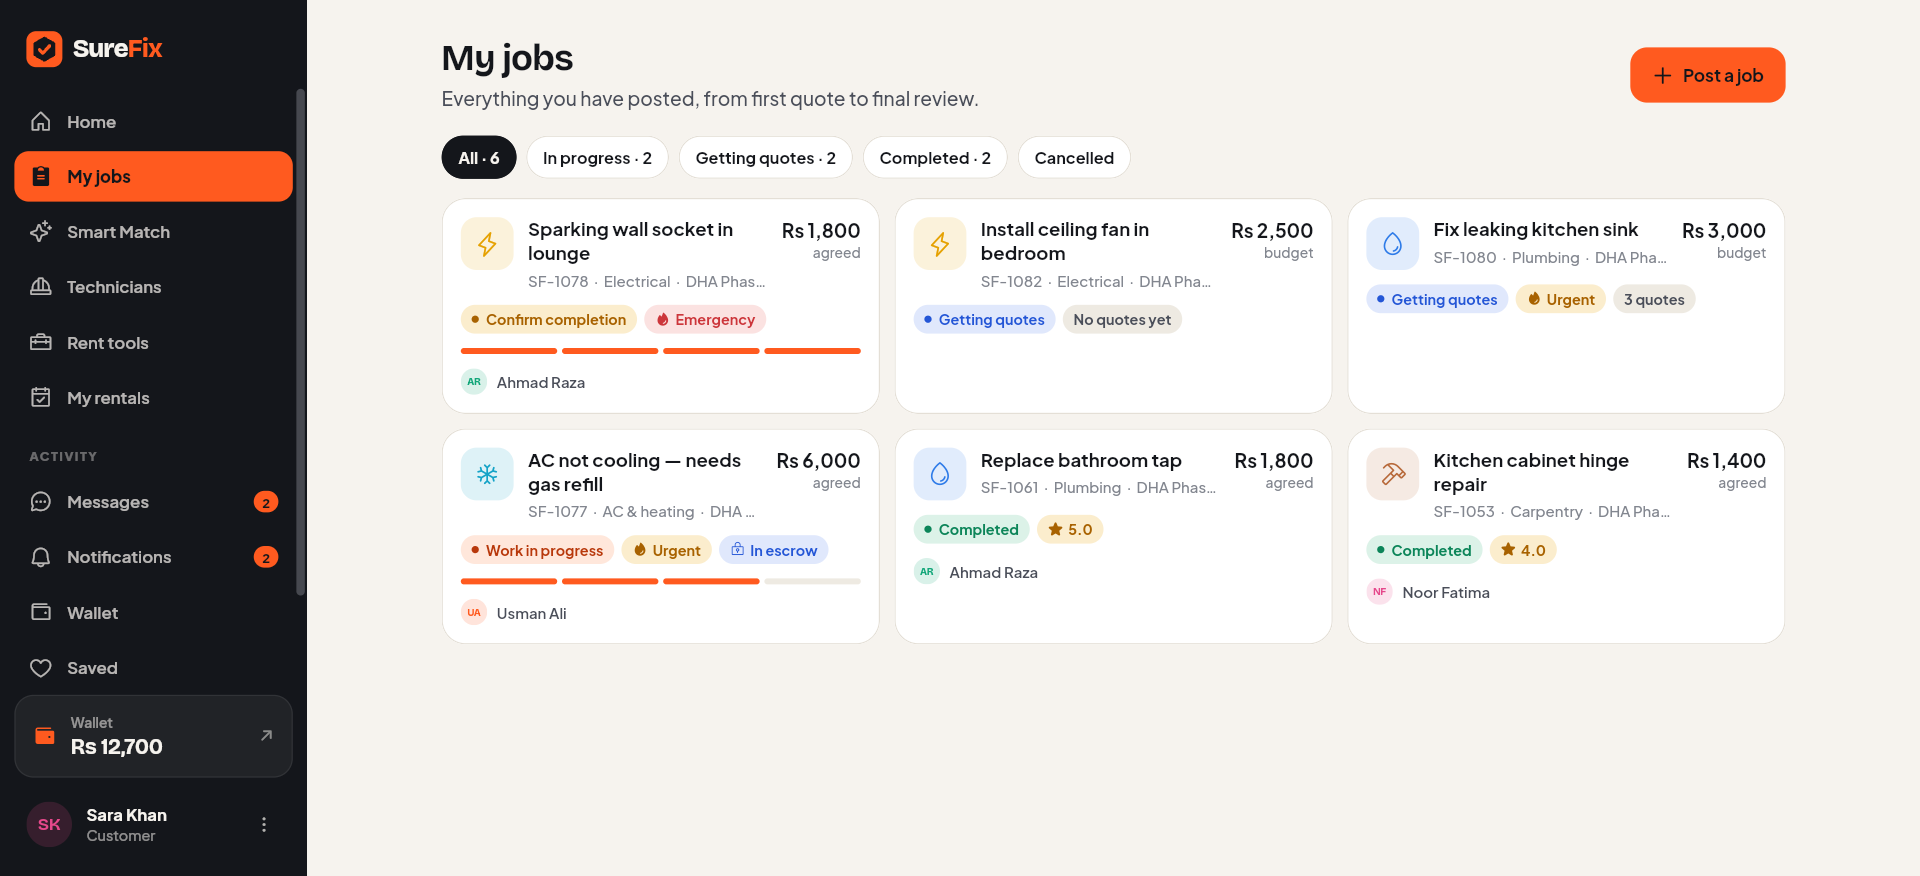
\includegraphics[width=1\linewidth]{clientscreen.png}
        \caption{This screen displays all jobs posted by the client with their number, status, stage, payment state and quotes, filtered by status.}
    \label{fig:placeholder}
\end{figure}

\textbf{Post Job Screen}

\begin{figure}[h]
    \centering
    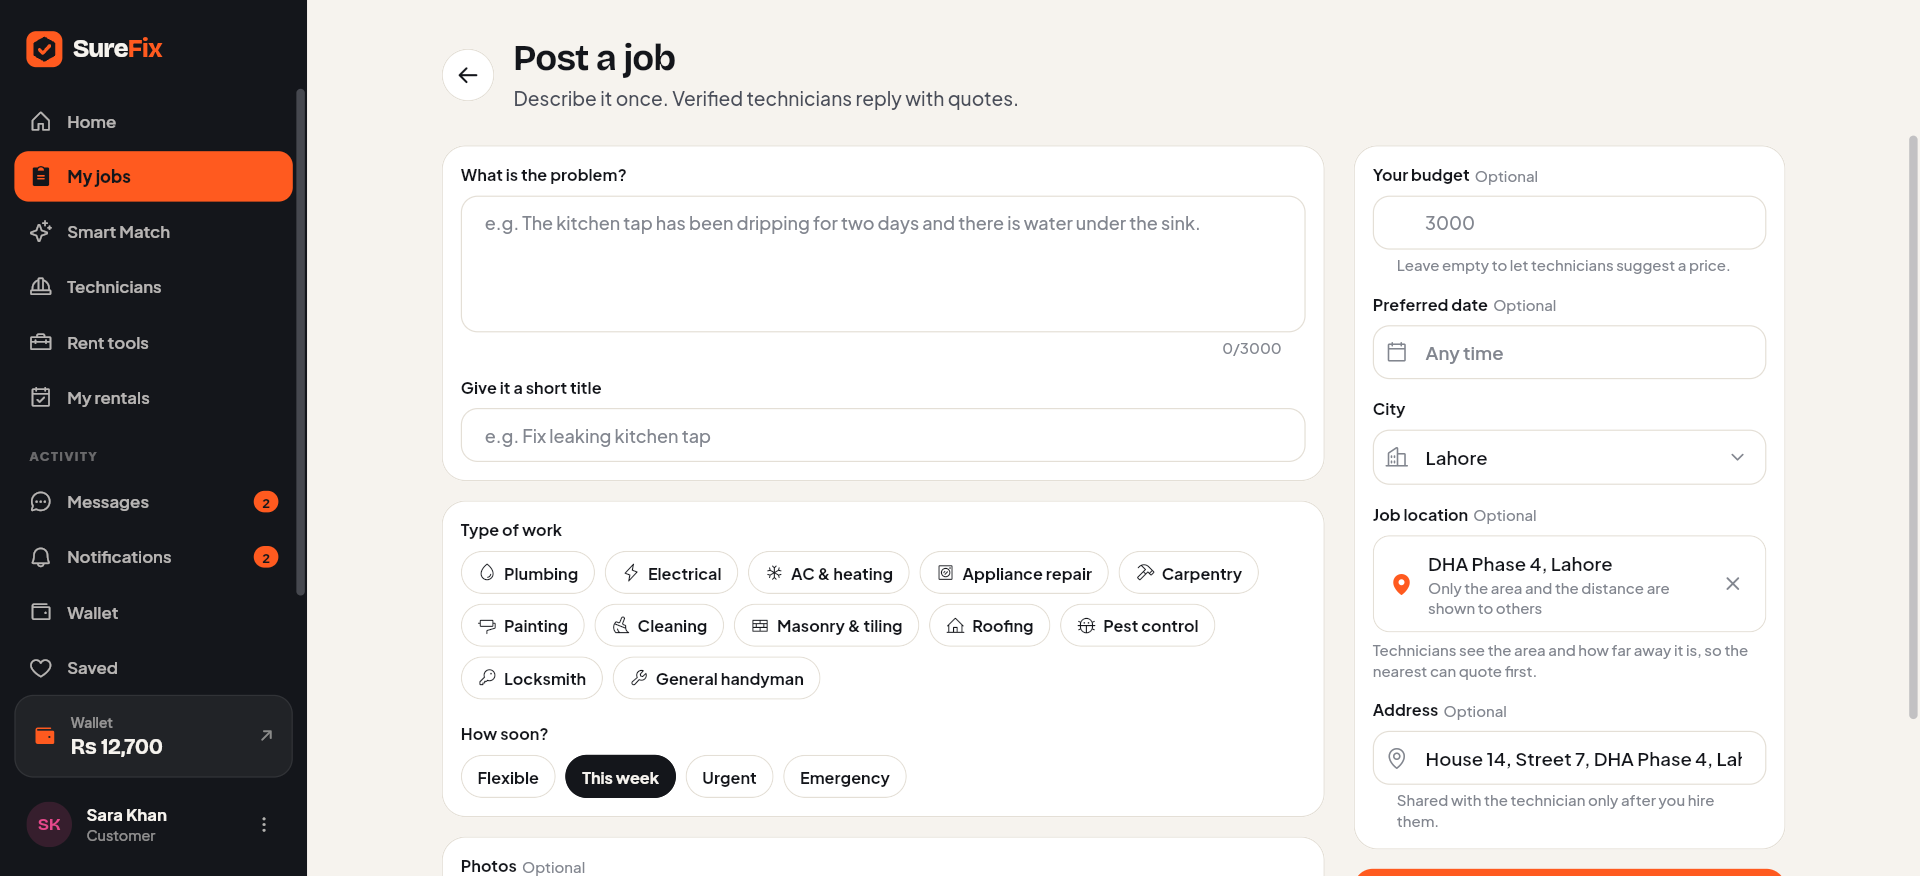
\includegraphics[width=1
    \linewidth]{job post desk.png}
        \caption{This screen allows clients to create a new job by describing the problem (the AI suggests the category and urgency), with budget, date, city and map location.}
    \label{fig:placeholder}
\end{figure}

\newpage

\textbf{Job Detail + Bids Screen}

\begin{figure}[H]
    \centering
    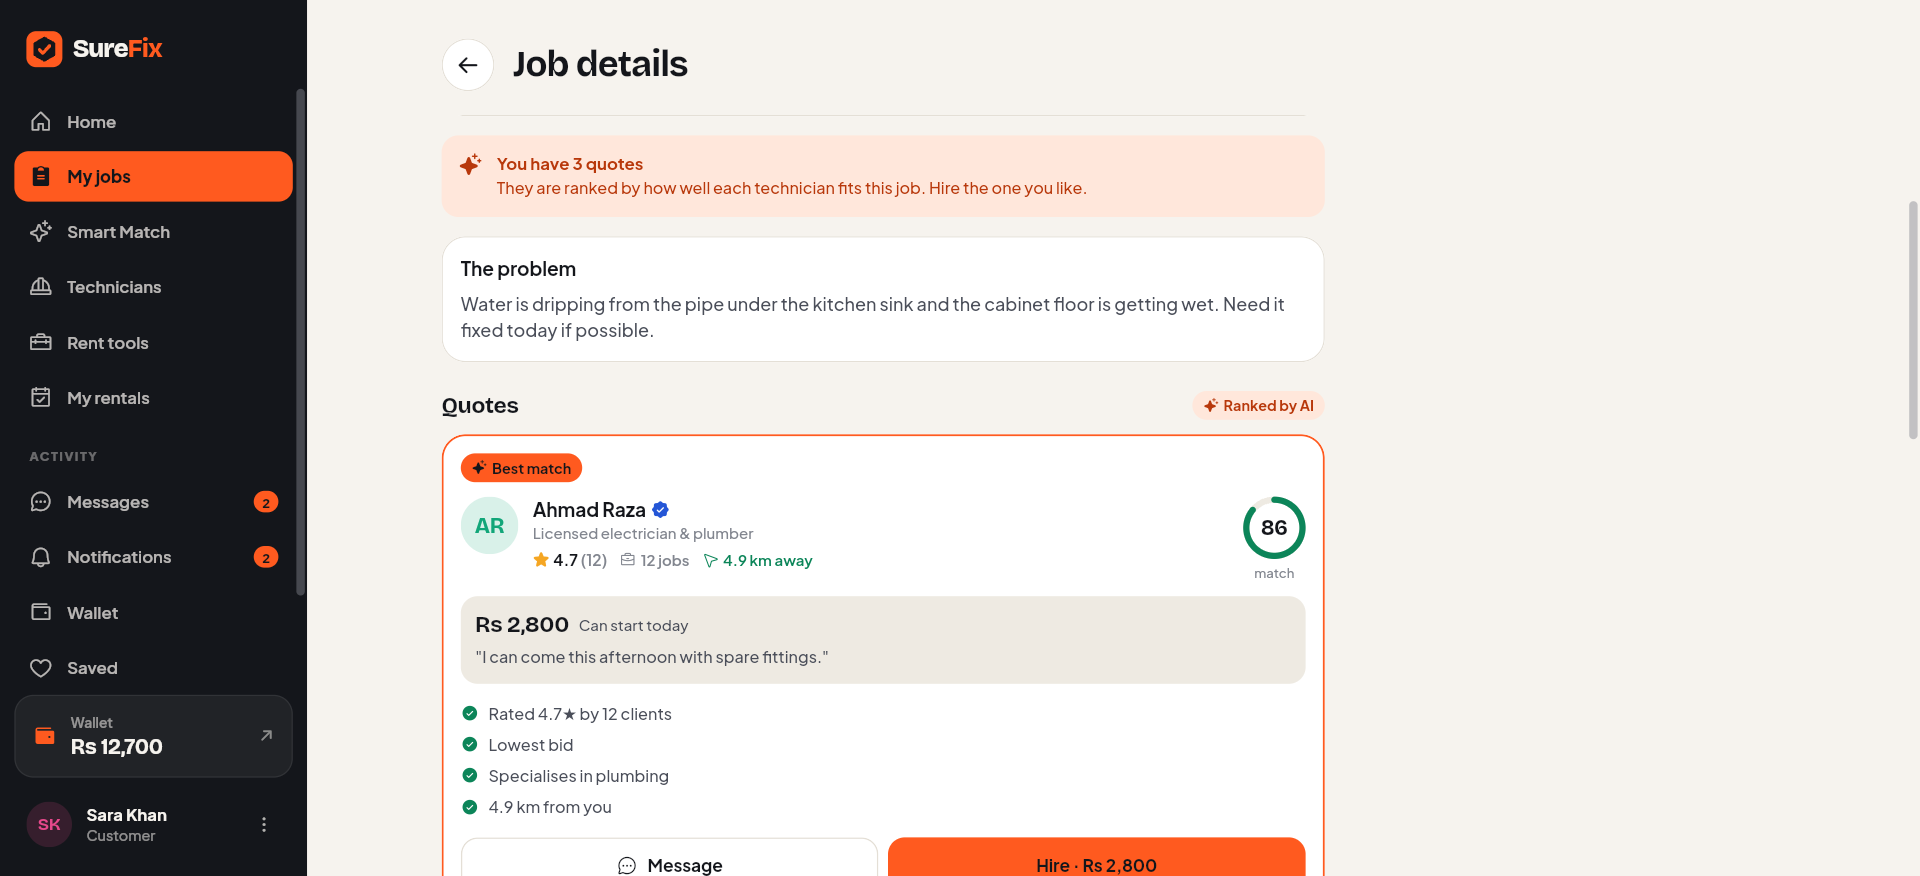
\includegraphics[width=1\linewidth]{job details.png}
        \caption{This screen shows the job with quotes ranked by AI: each shows a match percentage, the reasons and the distance, and the client can hire with one tap.}
    \label{fig:placeholder}
\end{figure}




\textbf{Bid Submission Screen}

\begin{figure}[h]
    \centering
    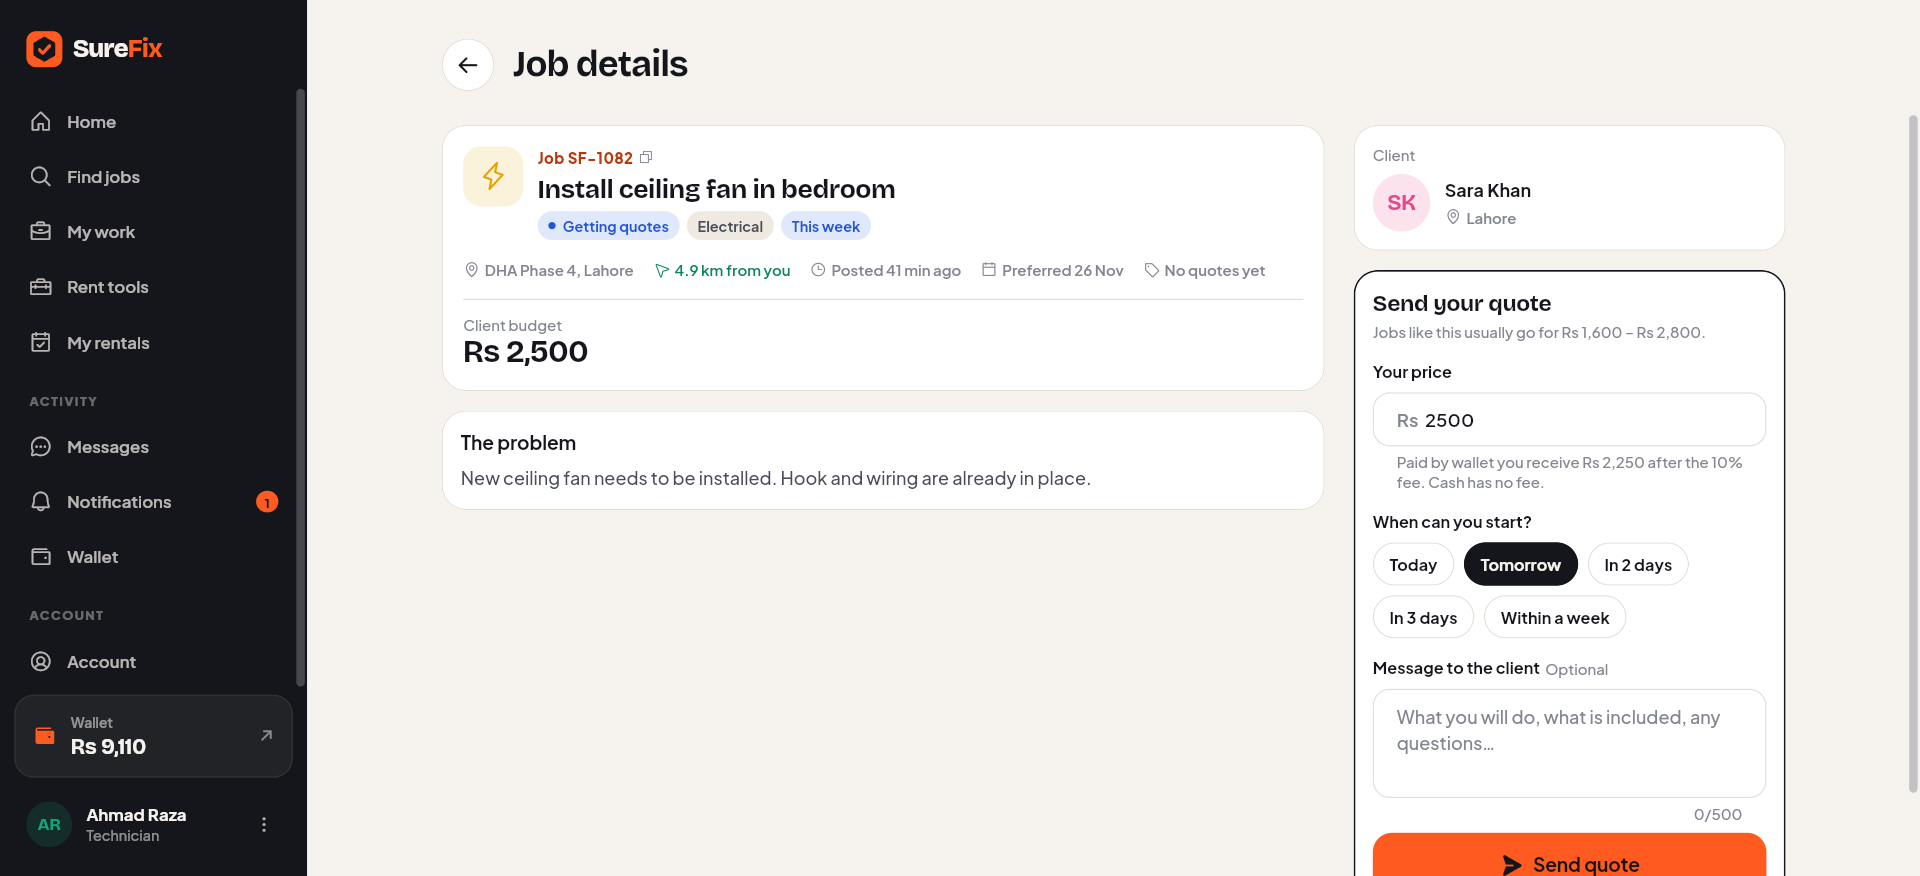
\includegraphics[width=1\linewidth]{bid.png}
        \caption{This screen allows technicians to send a quote with the price (with a fair-price hint and the fee shown), start time and a message.}
    \label{fig:placeholder}
\end{figure}

\newpage

\textbf{Tool Listing Screen}
\begin{figure}[H]
    \centering
    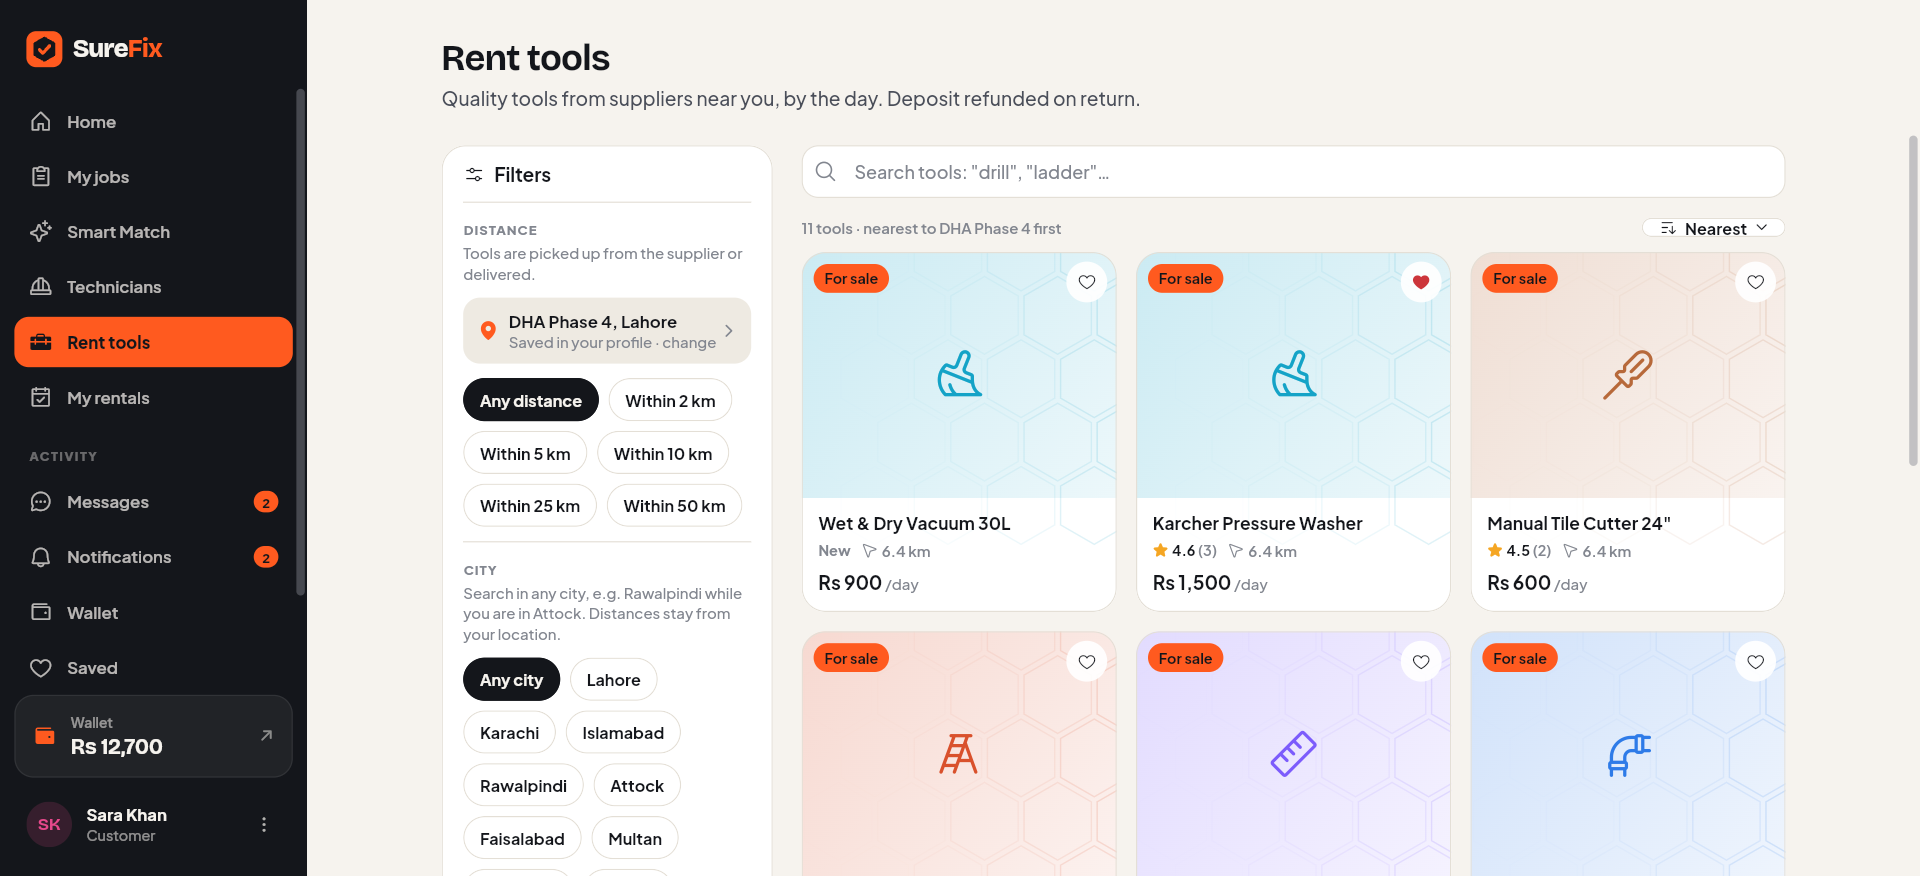
\includegraphics[width=1\linewidth]{tool.png}
        \caption{This screen displays tools near the user with distance, price per day and a For sale badge, with filters for distance, city, price and stock.}
    \label{fig:placeholder}
\end{figure}

\textbf{Admin Dashboard}
\begin{figure}[h]
    \centering
    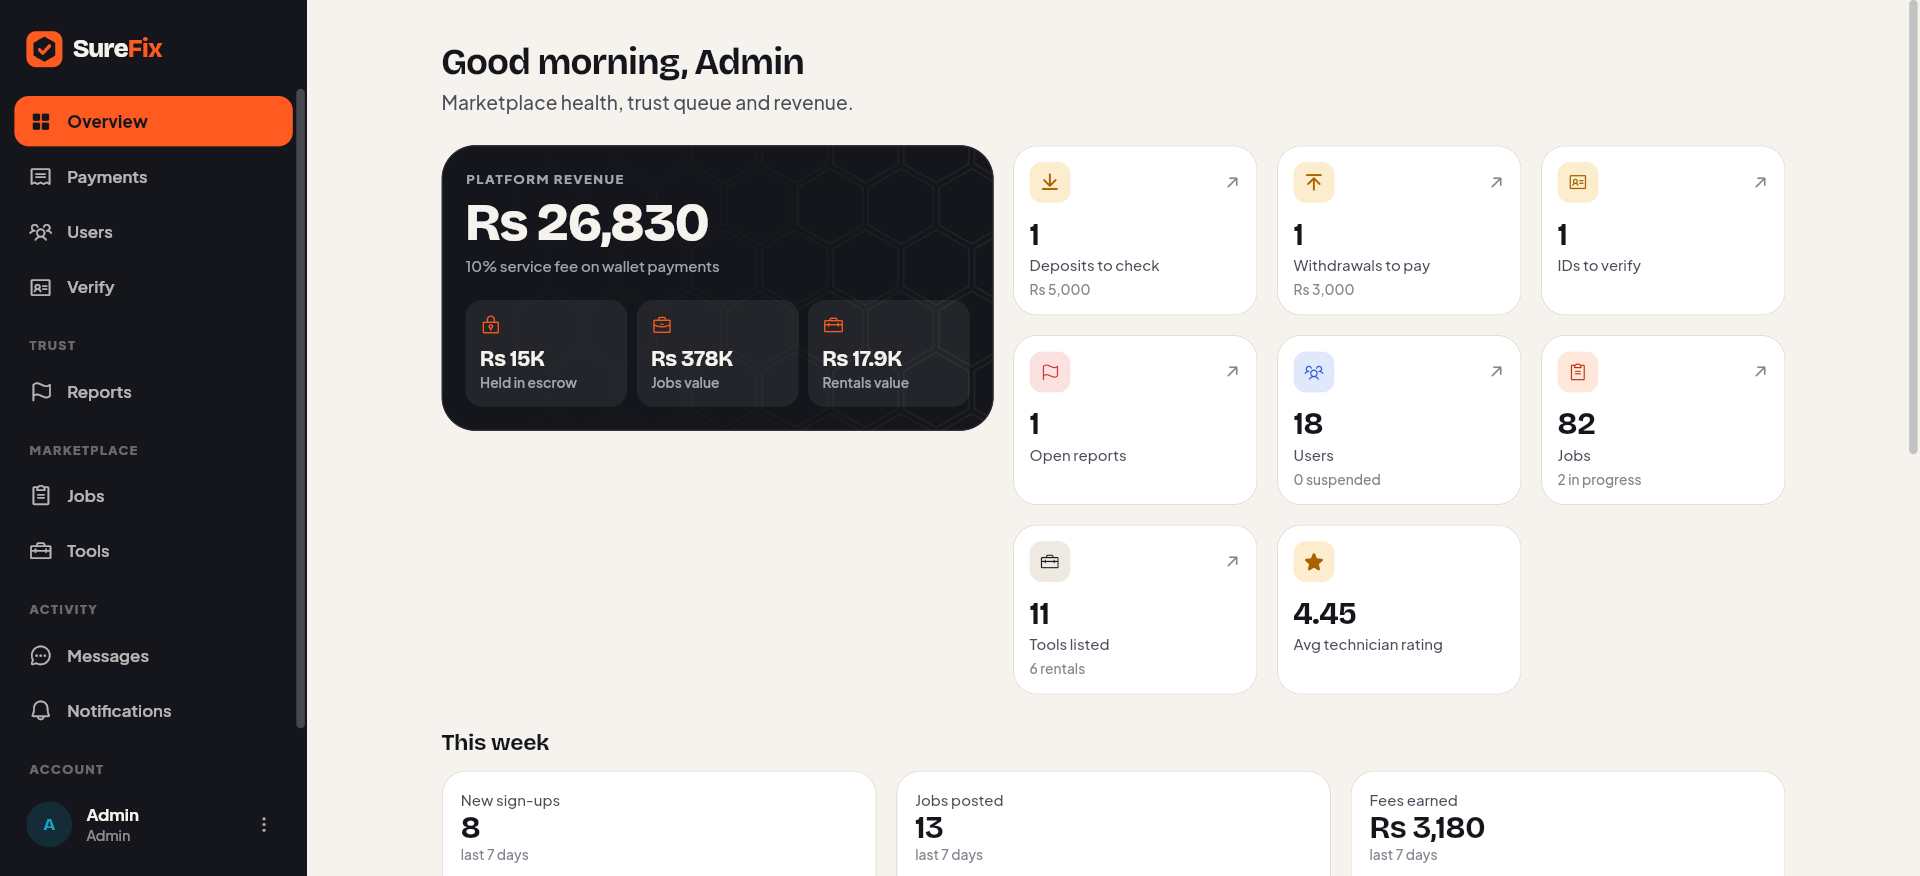
\includegraphics[width=1\linewidth]{admin.png}
        \caption{This screen allows the administrator to monitor revenue, escrow, deposits and withdrawals to review, KYC requests, reports and weekly activity.}
    \label{fig:placeholder}
\end{figure}

\newpage
\textbf{Tool Rent / Buy Screen}
\begin{figure}[H]
    \centering
    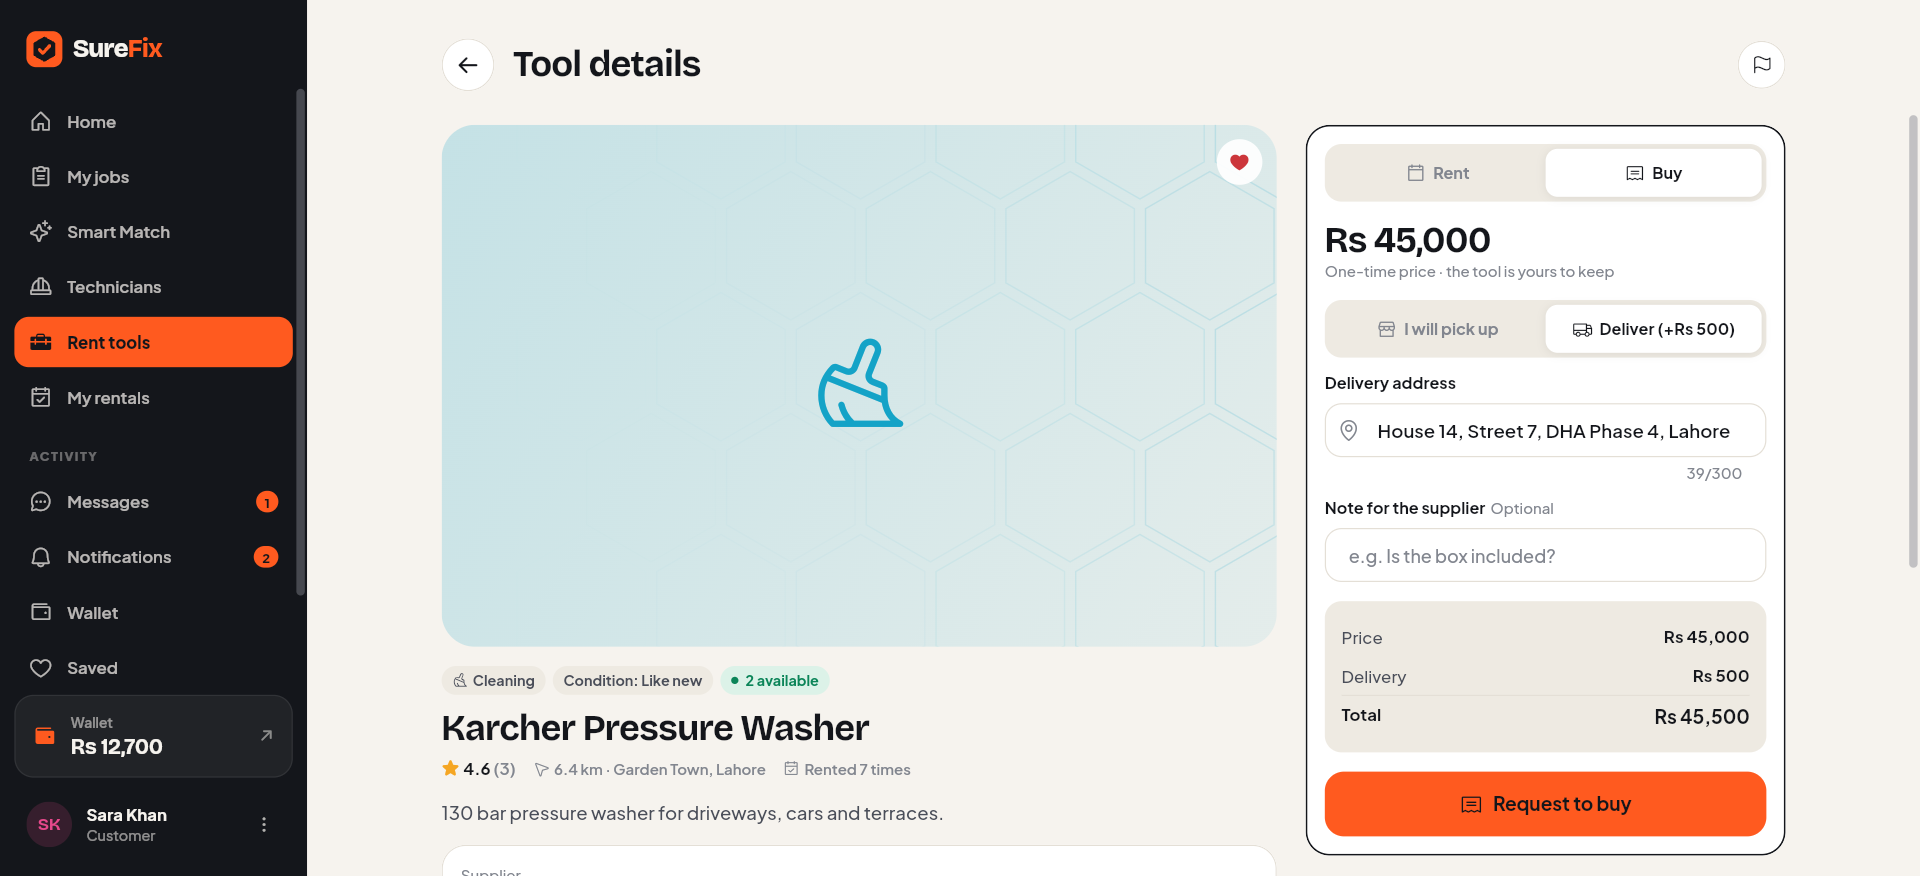
\includegraphics[width=1\linewidth]{tool_buy.png}
    \caption{This screen lets a customer rent a tool by the day or buy it for a one-time price, with pickup or delivery at the supplier's price.}
    \label{fig:placeholder}
\end{figure}

\textbf{Invoice Screen}
\begin{figure}[H]
    \centering
    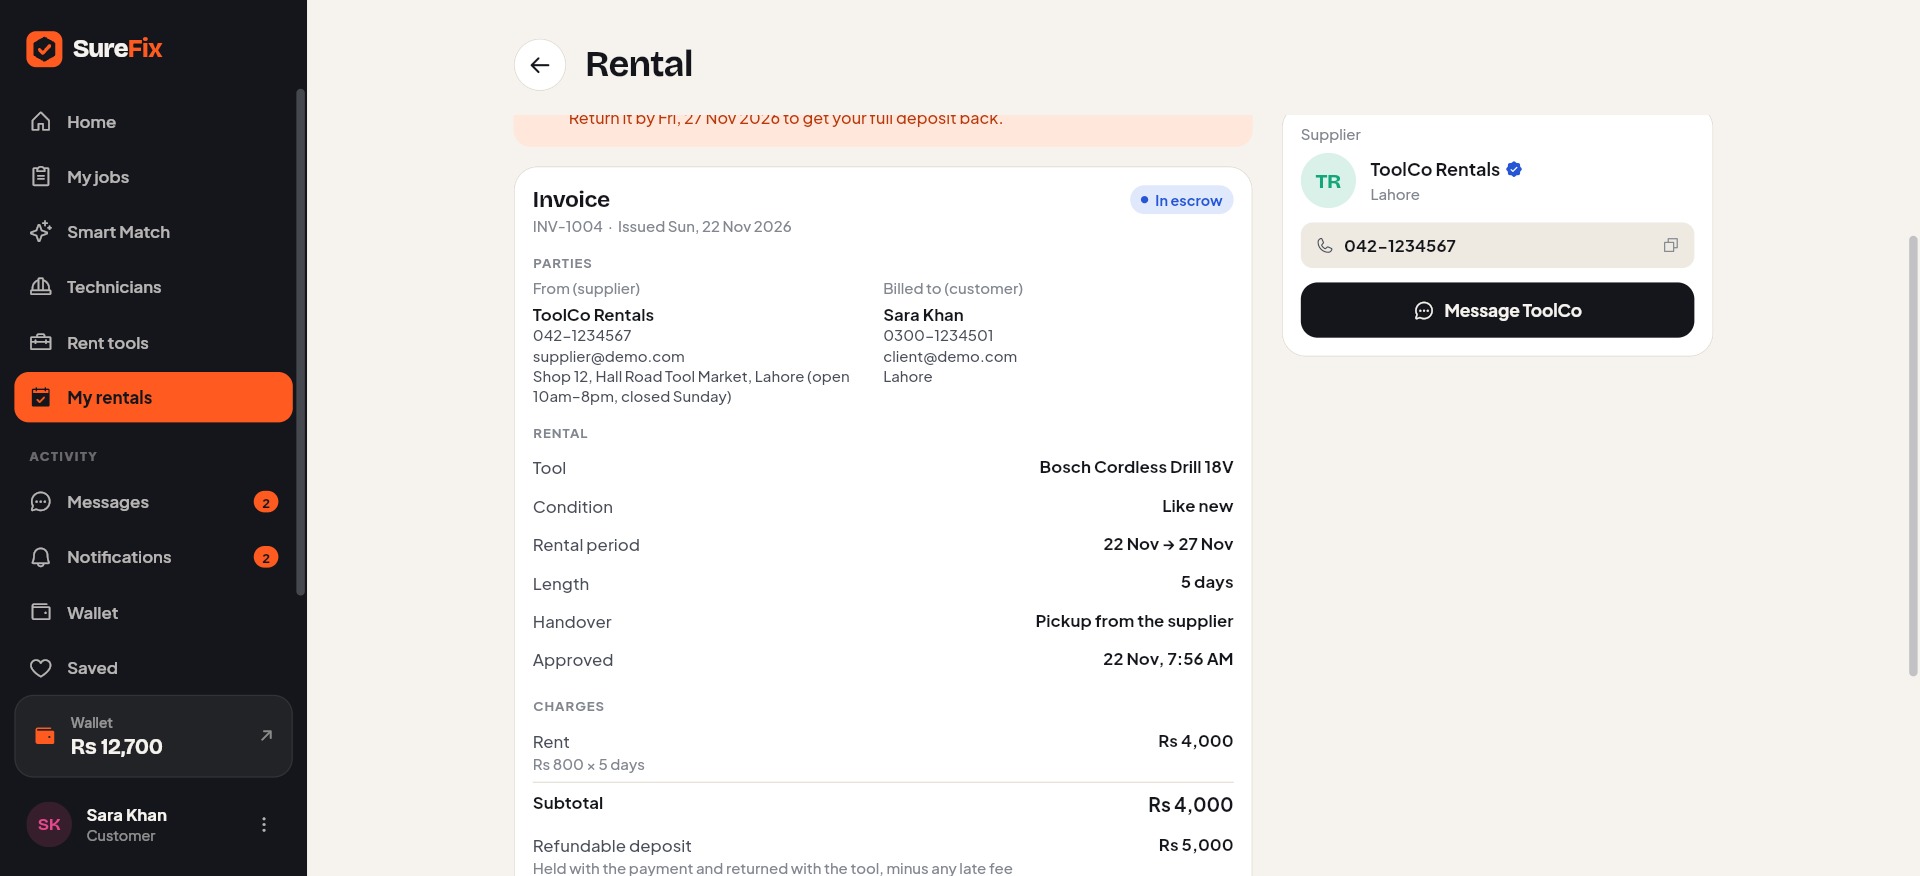
\includegraphics[width=1\linewidth]{invoice.png}
    \caption{This screen shows the detailed invoice of a rental or purchase: parties, dates, charges, deposit, late fee, refunds and payment status.}
    \label{fig:placeholder}
\end{figure}

\newpage
\textbf{Wallet Screen}
\begin{figure}[H]
    \centering
    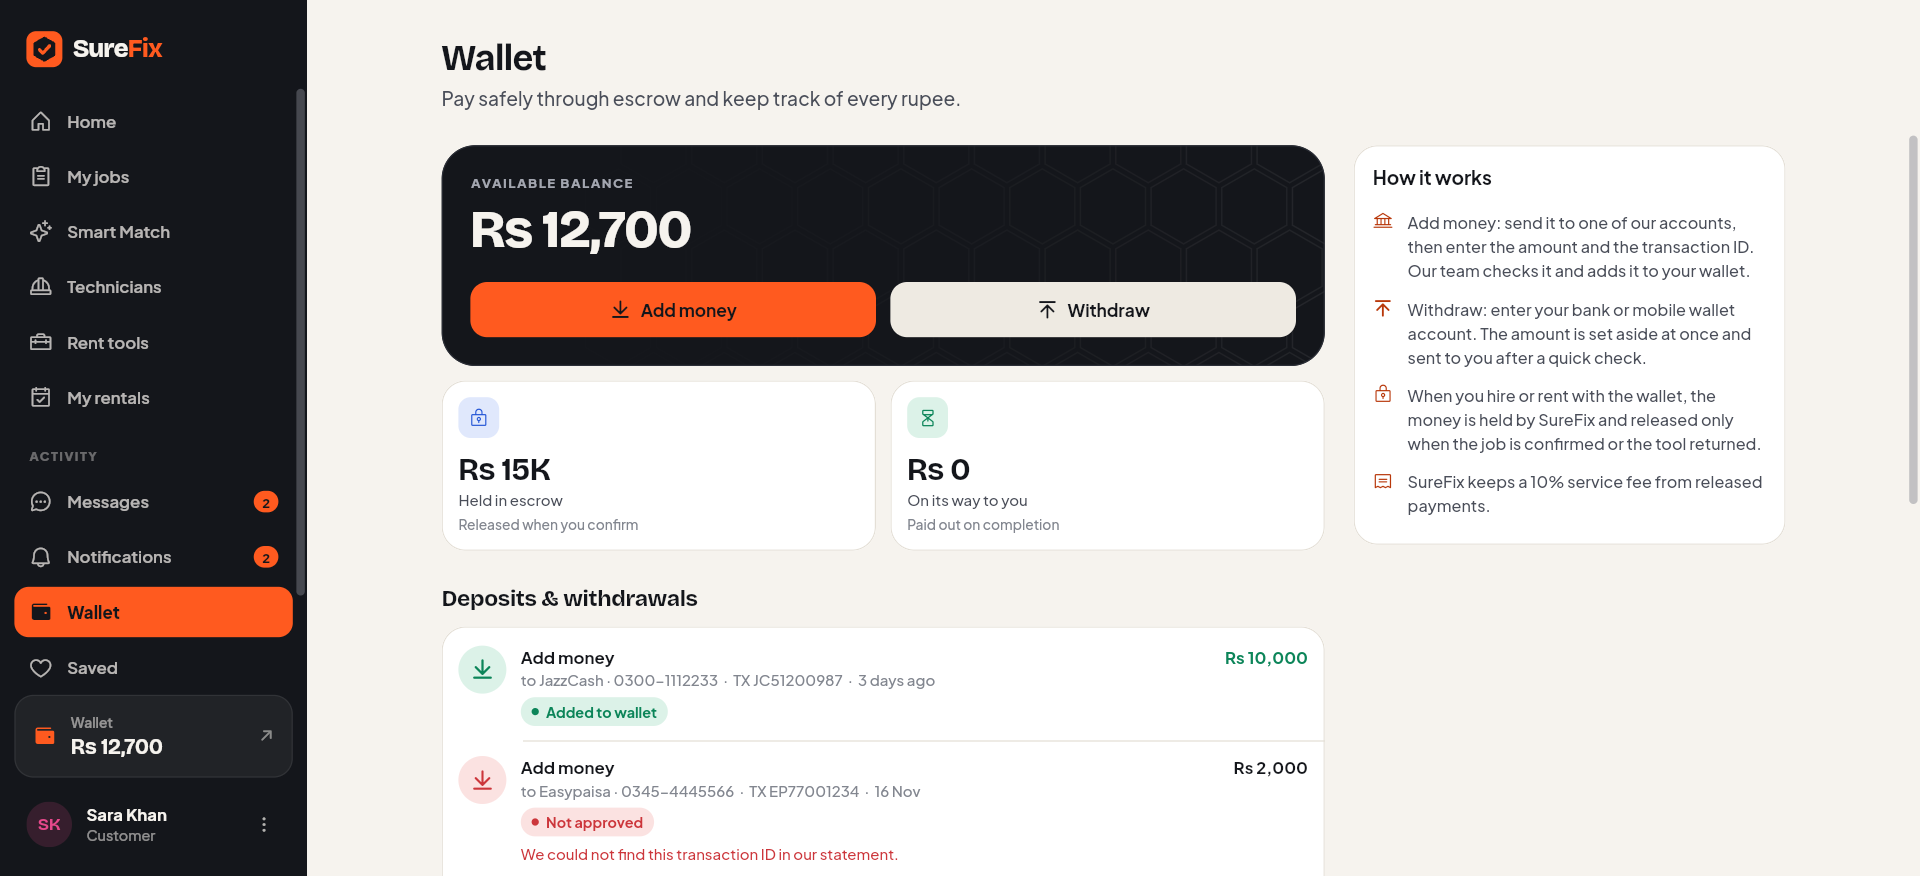
\includegraphics[width=1\linewidth]{wallet.png}
    \caption{This screen shows the wallet balance, money held in escrow, deposits and withdrawals with their review status, and the full history.}
    \label{fig:placeholder}
\end{figure}

\textbf{Messages Screen}
\begin{figure}[H]
    \centering
    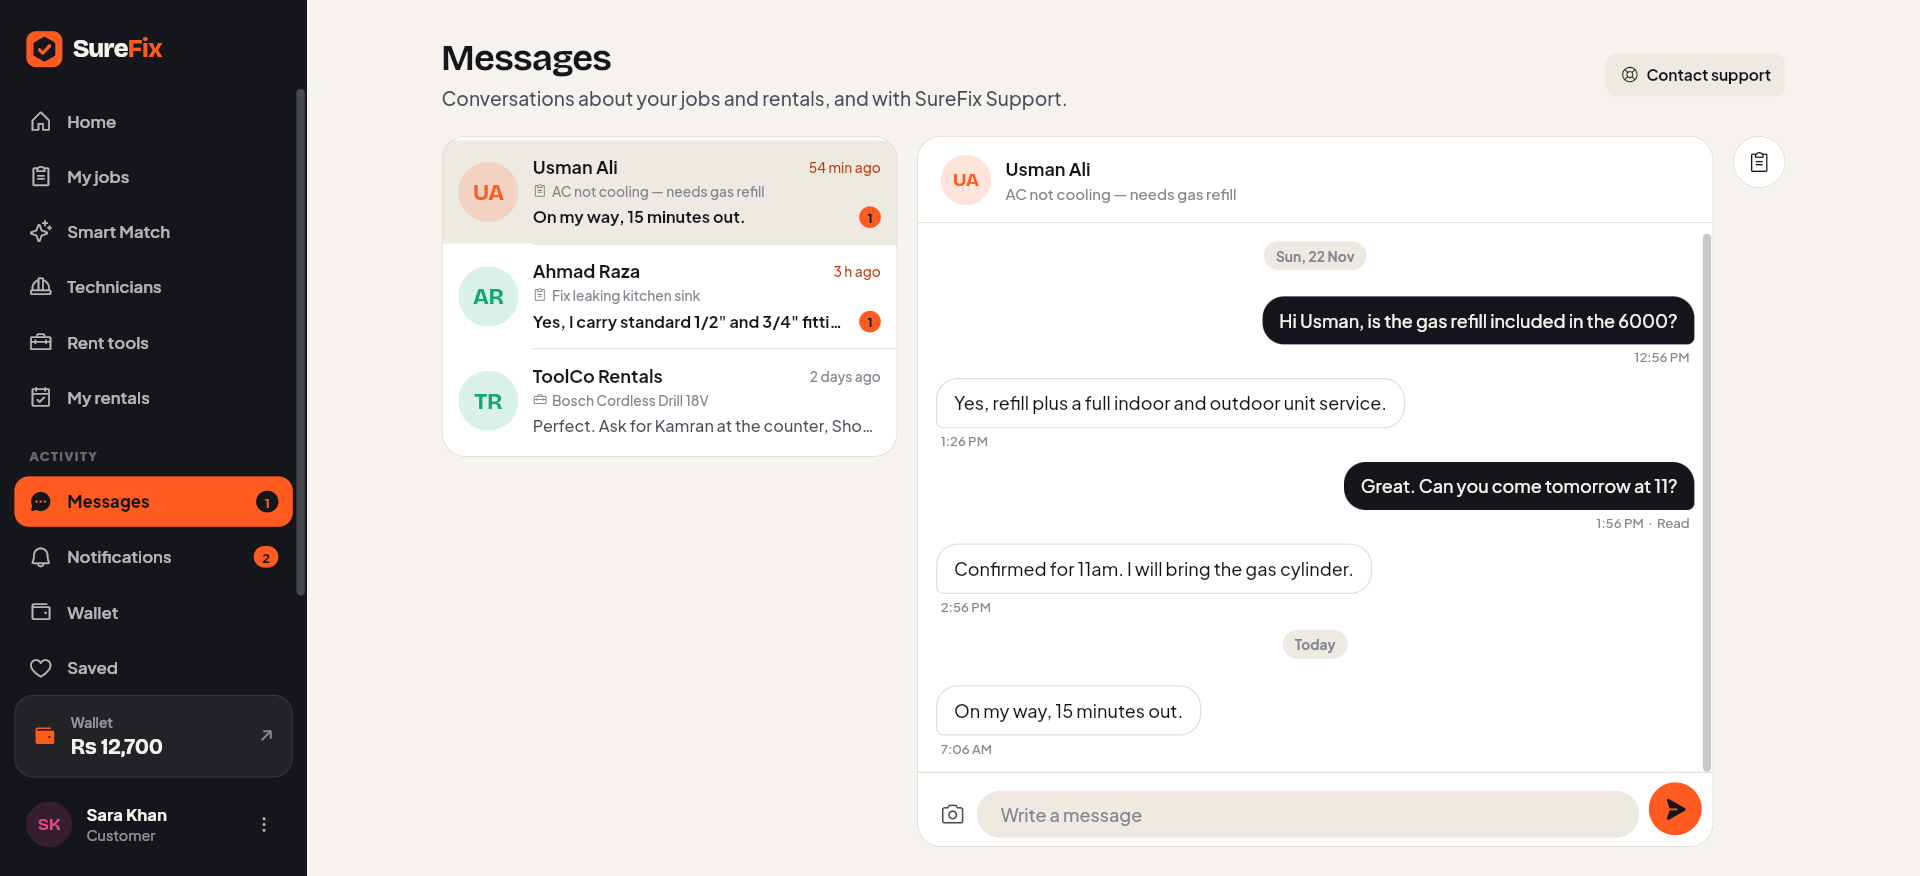
\includegraphics[width=1\linewidth]{chat.png}
    \caption{This screen shows real-time conversations about jobs and tools, and with SureFix Support, with photos and read receipts.}
    \label{fig:placeholder}
\end{figure}

\newpage
\textbf{Find Technicians Screen}
\begin{figure}[H]
    \centering
    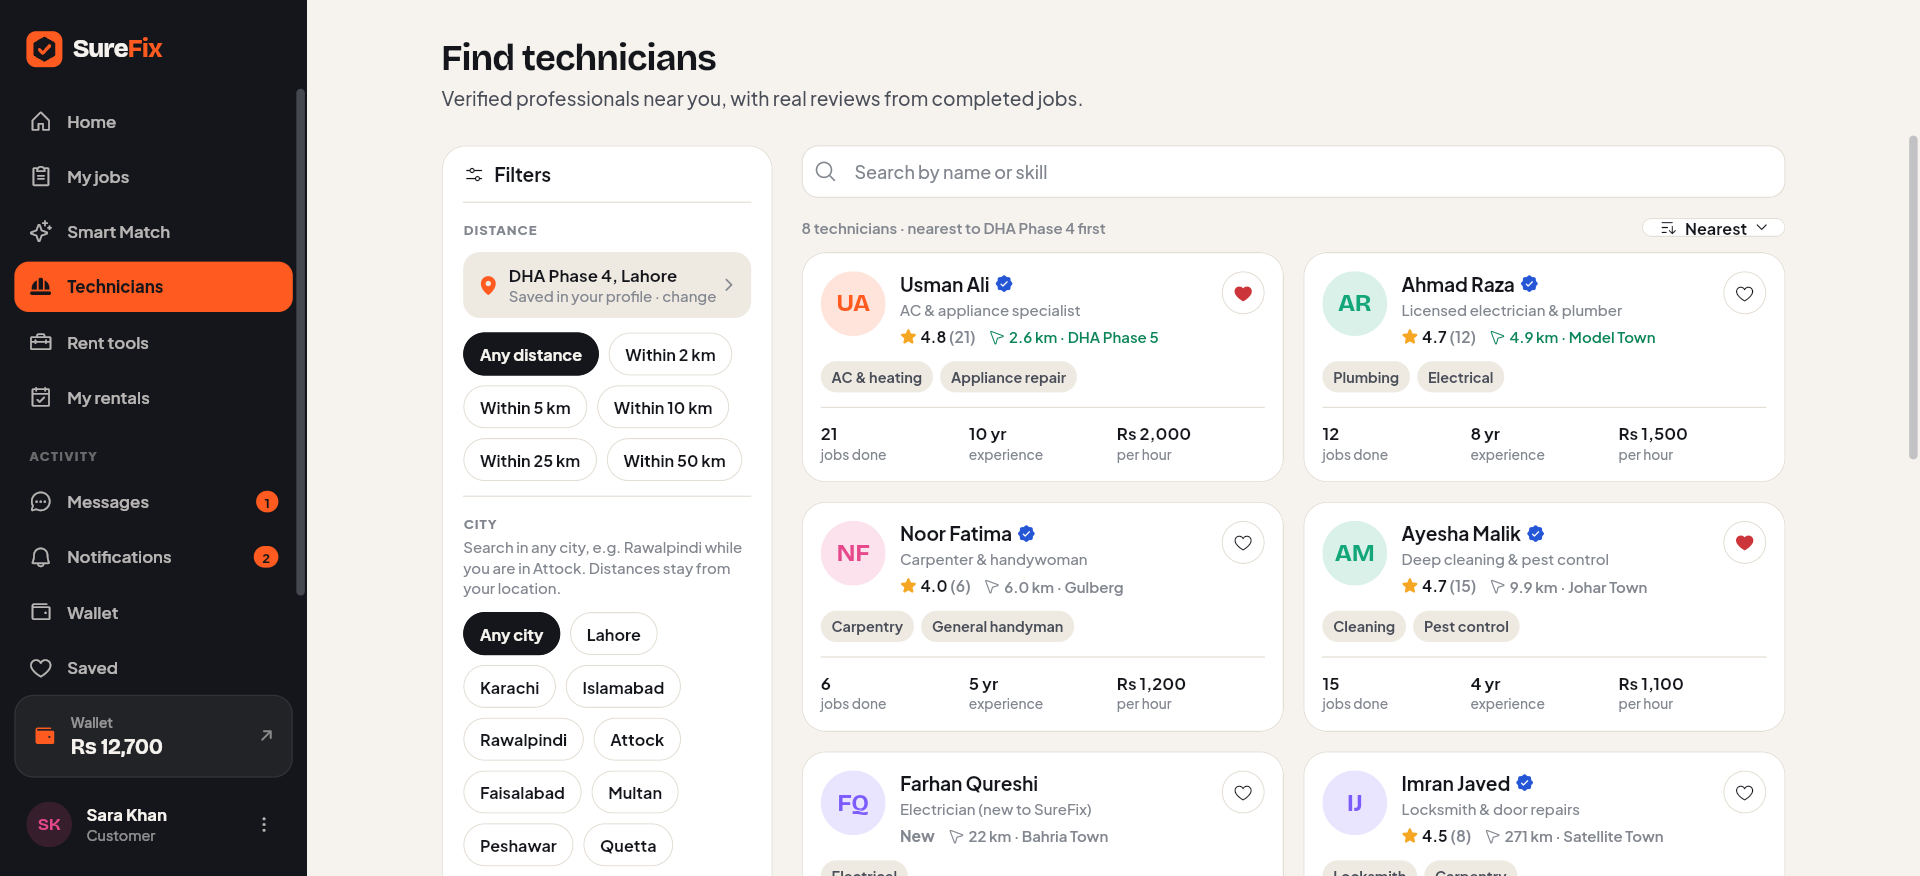
\includegraphics[width=1\linewidth]{technicians.png}
    \caption{This screen lists technicians nearest to the saved location first, with distance, rating, rates and filters for distance and city.}
    \label{fig:placeholder}
\end{figure}

\textbf{Supplier Orders Screen}
\begin{figure}[H]
    \centering
    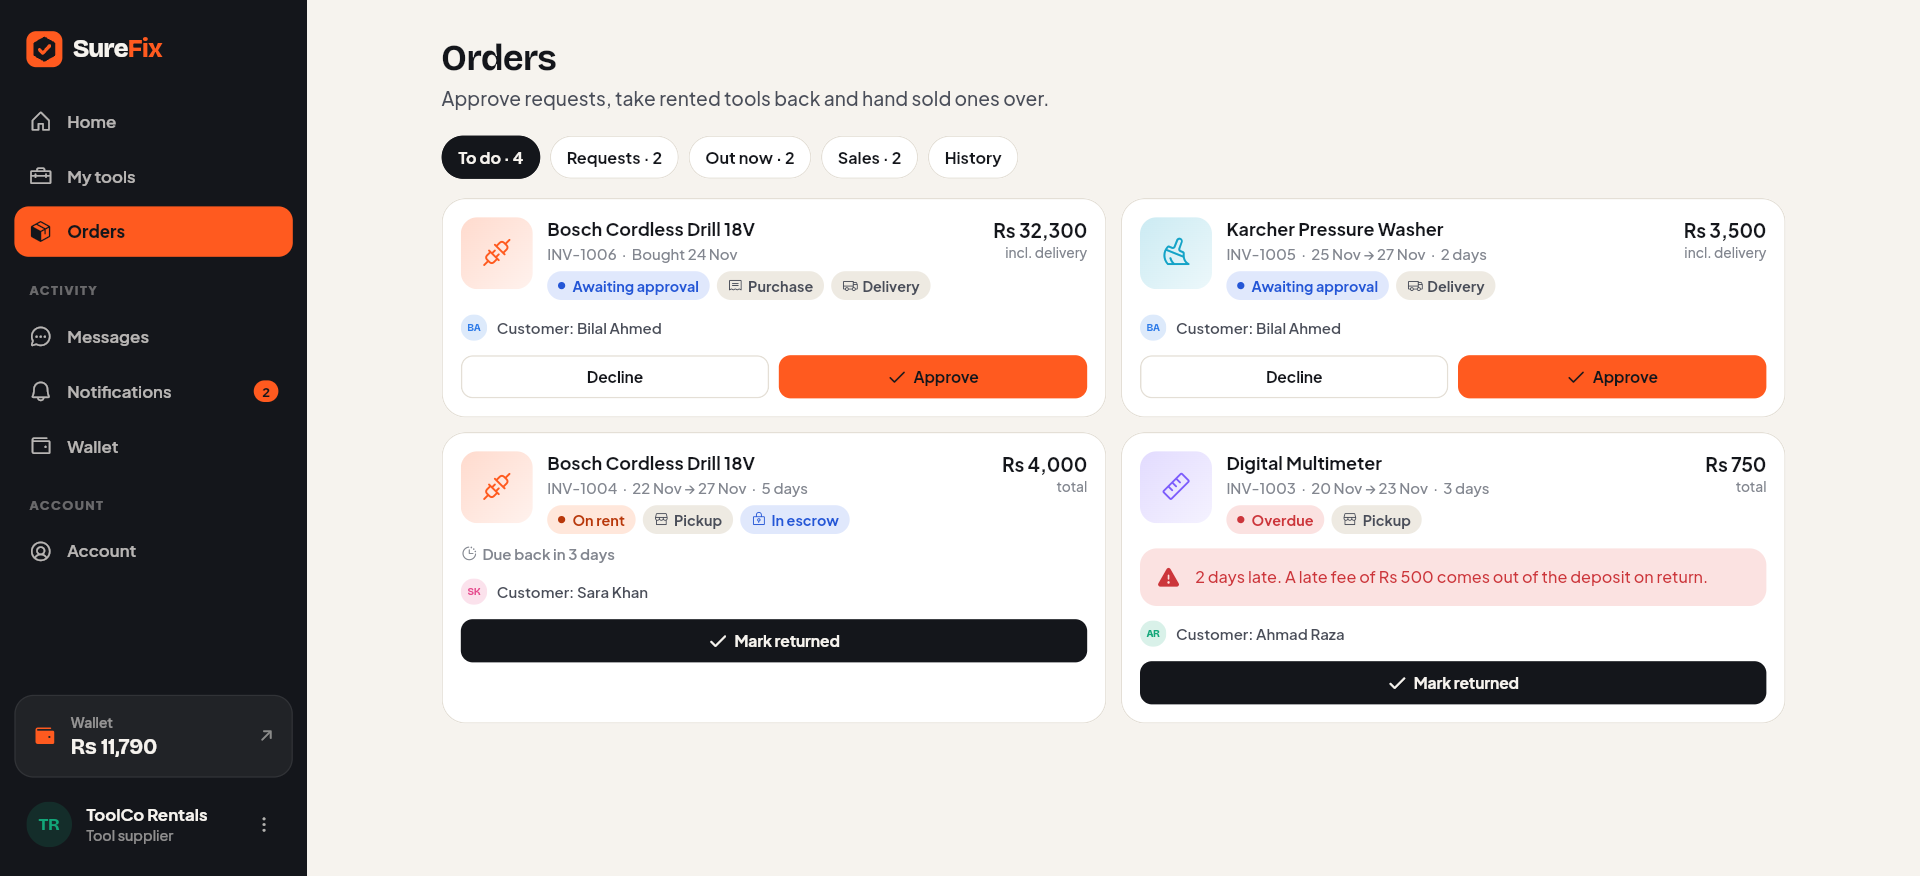
\includegraphics[width=1\linewidth]{supplier_orders.png}
    \caption{This screen lets suppliers approve or decline rental and purchase requests, mark rentals returned and hand sold tools over.}
    \label{fig:placeholder}
\end{figure}

\newpage
\textbf{Admin Company Accounts Screen}
\begin{figure}[H]
    \centering
    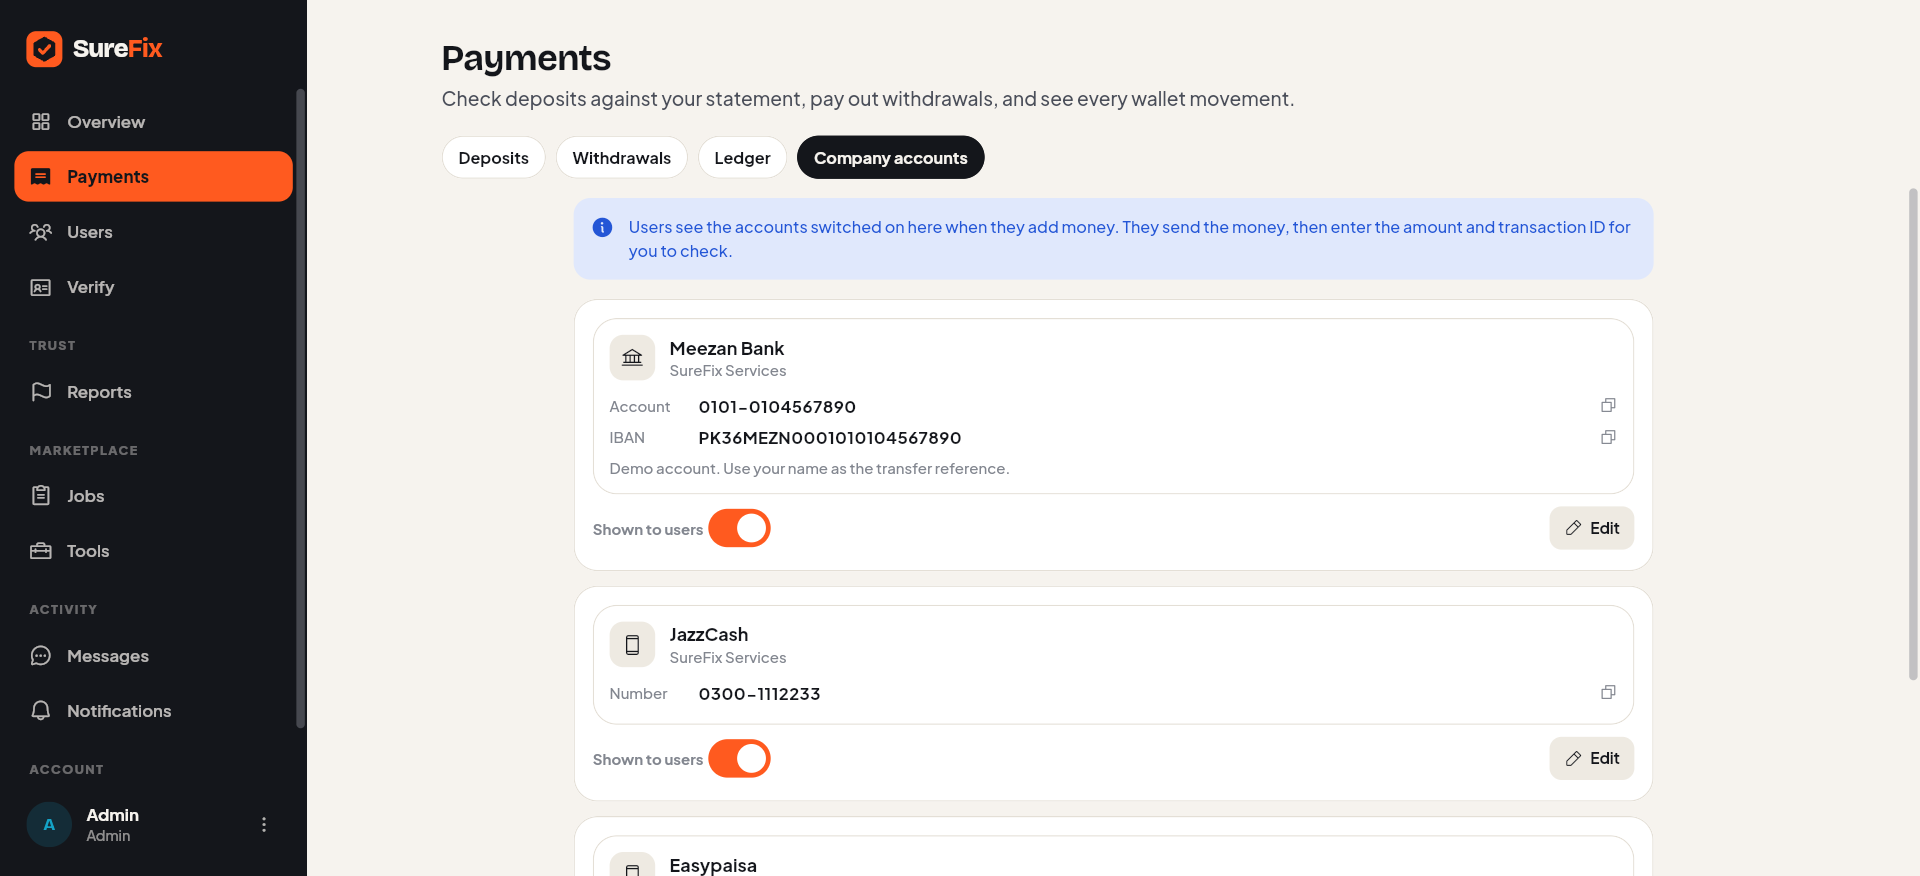
\includegraphics[width=1\linewidth]{admin_accounts.png}
    \caption{This screen lets the administrator add, edit, show or hide the company bank and mobile-wallet accounts that users send deposits to.}
    \label{fig:placeholder}
\end{figure}


\newpage
\subsection{Screen Objects and Actions}

This section provides a discussion of the primary screen objects and the actions associated with them in the SureFix system.

\begin{itemize}

\item \textbf{Authentication Screen}  

\textbf{Object:} Login and Registration forms with input fields (email, password, role selection) and the email confirmation step.

\textbf{Action:} The user enters credentials and submits the form, then confirms the email by link or code.

\textbf{System Response:} The system validates the input and redirects the user to the role-specific home screen or displays an error message.

\item \textbf{Navigation Sidebar / Dock}

\textbf{Object:} Sidebar (wide screens) or bottom dock (phones) with the role's sections and the account menu.    

\textbf{Action:} The user selects any option from the drawer.  

\textbf{System Response:} The system navigates to the selected screen or performs the logout action.

\item \textbf{Job Posting Form}  

\textbf{Object:} Input fields for description, title, category, urgency, budget, preferred date, photos, city and location.    

\textbf{Action:} The client fills in the form and submits it.  

\textbf{System Response:} The system validates the input, creates the job with its number, notifies technicians, and displays a success message.

\item \textbf{Bidding Interface}  

\textbf{Object:} Quote form with fields for price, start time, and message.    

\textbf{Action:} The technician submits a bid for a job.  

\textbf{System Response:} The system records the bid, updates the job details, and notifies the client.

\item \textbf{Job Detail Screen}  

\textbf{Object:} Displays job information, AI-ranked quotes, stages and action buttons (Hire, Confirm job is done, Rate).    

\textbf{Action:} The client or technician performs actions such as accepting a bid or updating job status.  

\textbf{System Response:} The system updates the job status and sends real-time notifications to relevant users.

\item \textbf{Tool Listing Screen}  

\textbf{Object:} List of available tools and the tool page with Rent / Buy, pickup or delivery, and the price summary.

\textbf{Action:} The user requests to rent or buy a tool and chooses wallet or cash.

\textbf{System Response:} The system holds a wallet payment, notifies the supplier, reserves stock on approval, and issues an invoice.

\item \textbf{Messaging Screen}  

\textbf{Object:} Chat interface showing conversation between users.  

\textbf{Action:} The user sends a message.  

\textbf{System Response:} The message is delivered instantly and displayed in real-time for both users.

\item \textbf{Notification System}  

\textbf{Object:} Notification panel and toast messages.  

\textbf{Action:} This is a read-only component for users.  

\textbf{System Response:} The system displays real-time updates such as new bids, job status changes, and tool rentals.

\item \textbf{Logout Button}  

\textbf{Object:} Logout option in the account menu.    

\textbf{Action:} The user clicks logout.  

\textbf{System Response:} The system clears the session, disconnects real-time services, and redirects to the login screen.

\item \textbf{Wallet Screen}

\textbf{Object:} Balance, escrow summary, Add money and Withdraw buttons, request list and history.

\textbf{Action:} The user submits a deposit (amount and transaction ID) or a withdrawal.

\textbf{System Response:} The request waits for admin review; the user is notified when it is approved or rejected.

\end{itemize}

\section{System Algorithms}

The system’s functionality is driven by backend processing and an AI-based ranking algorithm that supports decision-making.

\subsubsection{Algorithm 1: Main System Controller (Backend Server)}

This is the high-level control logic implemented in the Node.js backend.

\begin{itemize}
    \item \textbf{Wait for Request:} The server listens for API requests from the mobile application.
    
        \item \textbf{Authenticate User:} Validates JWT sessions (issued after a verified Firebase sign-in) for secure access.
    
        \item \textbf{Process Request:} Executes operations such as job posting, bidding, hiring, wallet holds and releases, or tool rental and purchase.
    
    \item \textbf{Database Interaction:} Stores and retrieves data from MongoDB.
    
    \item \textbf{Trigger Events:} Sends real-time updates using Socket.IO.
    
    \item \textbf{Return Response:} Sends results back to the client in JSON format.
\end{itemize}

\subsubsection{Algorithm 2: AI-Based Technician Ranking}

This algorithm evaluates and ranks technicians based on performance metrics.

\begin{itemize}
        \item \textbf{Input Data:} Skills, rating and number of reviews, jobs assigned and completed, average response time, experience, distance, availability, verification and, for quotes, the price and the client's budget.

    \item \textbf{Normalisation:} Each factor becomes a component between 0 and 1. The rating is Bayesian-smoothed, $(r \cdot n + 3.5 \cdot 3)/(n+3)$, so a few reviews cannot dominate; proximity is $1/(1+d/8)$ for a distance $d$ in km.

    \item \textbf{Weighted Scoring:} For quotes the weights are skill 0.16, rating 0.22, reliability 0.14, responsiveness 0.08, experience 0.08, price 0.17, proximity 0.10 and verification 0.05; for recommendations, skill 0.28 and rating 0.20 lead. Urgent jobs boost responsiveness and availability.

    \item \textbf{Score Calculation:} The weighted sum gives a match percentage (0–100) and a score (0–5), and the strongest components become plain-language reasons.

    \item \textbf{Ranking and Output:} Technicians or quotes are sorted by score and returned to the client with their reasons.
\end{itemize}


\section{Tools and Technologies}

The following tools and technologies were used in the development of the SureFix system \cite{13,14,15,16,17}:

\begin{table}[H]
\centering
\caption{Tools and Technologies Used}
\begin{tabular}{|p{0.28\textwidth}|p{0.18\textwidth}|p{0.44\textwidth}|}
\hline
\textbf{Tools and Technologies} & \textbf{Version} & \textbf{Rationale (Purpose/Justification)} \\ \hline

Node.js & 22 LTS & Runtime environment for backend server; supports scalable and non-blocking API handling. \\ \hline

Express.js & 5.2.1 & Framework for building REST APIs and managing routing and middleware. \\ \hline

Socket.IO & 4.7.5 & Enables real-time communication for messaging and notifications. \\ \hline

MongoDB & Atlas / 7 & NoSQL database for storing users, jobs, bids, tools, and transactions, with geospatial indexes. \\ \hline

Mongoose & 8.0.3 & ODM for schema validation and structured database interaction. \\ \hline

Python & $\geq$3.10 & Used for implementing AI classification and ranking in the microservice. \\ \hline

FastAPI & $\geq$0.109 & High-performance framework for building AI service APIs. \\ \hline

Flutter & 3.35 & Cross-platform framework for building the Android app and the website. \\ \hline

Dart SDK & $\geq$3.1.0 <4.0.0 & Programming language used with Flutter for frontend development. \\ \hline

JWT (jsonwebtoken) & 9.0.2 & Provides secure session authorization across the system. \\ \hline

Firebase Authentication & firebase\_auth 7 / firebase-admin 13 & Sign-in, email verification and password-reset emails. \\ \hline

Jest / flutter\_test / pytest & 29 / SDK / 8 & Automated test suites for backend, app and AI service. \\ \hline

GitHub Actions & -- & Continuous integration, website publishing and APK builds. \\ \hline

\end{tabular}
\end{table}



\section{External APIs / SDKs}

This section describes the major third-party APIs (Application Programming Interfaces) and SDKs (Software Development Kits) used in the implementation of the SureFix system.

\begin{table}[H]
\centering
\caption{External APIs / SDKs Used in Implementation}
\begin{tabular}{|p{0.3\textwidth}|p{0.18\textwidth}|p{0.42\textwidth}|}
\hline
\textbf{API / SDK Name} & \textbf{Version} & \textbf{Purpose in Project} \\ \hline

Express.js & \textasciicircum{}5.2.1 & Used as the backend web framework to build REST APIs and handle HTTP requests and routing. \\ \hline

Socket.IO & \textasciicircum{}4.7.5 & Provides real-time bidirectional communication for chat, notifications, and live updates. \\ \hline

Mongoose & \textasciicircum{}8.0.3 & ODM SDK used for schema-based data modeling and interaction with MongoDB. \\ \hline

FastAPI & $\geq$0.109 & Used to build the AI microservice with high-performance asynchronous APIs. \\ \hline

Pydantic & $\geq$2.5 & Provides data validation and serialization in the FastAPI-based AI service. \\ \hline

Uvicorn & $\geq$0.27 & ASGI server used to run the FastAPI application efficiently. \\ \hline

Flutter SDK & 3.35 & Used to build the Android app and the website with a single codebase. \\ \hline

Firebase Auth / Core (Dart) & \textasciicircum{}7.0.1 / \textasciicircum{}5.1.0 & Email sign-in, verification and password reset in the app. \\ \hline

firebase-admin (Node) & \textasciicircum{}13.10.0 & Verifies Firebase ID tokens and copies accounts on the server. \\ \hline

flutter\_map + latlong2 & \textasciicircum{}8.3.2 / \textasciicircum{}0.10.1 & OpenStreetMap map picker for saved locations. \\ \hline

geolocator & \textasciicircum{}14.0.2 & Reads the device location for near-me search. \\ \hline

flutter\_local\_notifications & \textasciicircum{}20.1.0 & Phone notifications in the notification bar, with sound. \\ \hline

image\_picker & \textasciicircum{}1.1.2 & Photos for jobs, proof of work, KYC and chat. \\ \hline

Nodemailer & \textasciicircum{}6.9.16 & Sends verification and reset codes when Firebase is not used. \\ \hline

Helmet / express-rate-limit & \textasciicircum{}8.3.0 / \textasciicircum{}7.5.1 & Security headers and rate limiting. \\ \hline

Dart HTTP Package & \textasciicircum{}1.1.2 & Enables REST API communication between Flutter frontend and Node.js backend. \\ \hline

Socket.IO Client (Dart) & \textasciicircum{}2.0.3+1 & Connects Flutter app to backend for real-time messaging and updates. \\ \hline

\end{tabular}
\end{table}

\section{User Interface}

This section provides details and descriptions of the user interface for the SureFix system’s sub-systems.

The system consists of multiple sub-systems: the Flutter Application (Android app and website), a Backend Server, and the Admin Portal inside the same application. All user interactions occur through the application, which provides role-based interfaces for clients, technicians, suppliers and administrators.

\subsection{Mobile Application: Authentication Interface}

This is the entry point of the application, as shown in Figure X.X.

-- \textbf{Description:} This screen allows users to log in or register using email and password. Users select their role (client, technician, or supplier) during registration and confirm their email before the first login.

-- \textbf{Features:} It includes input validation, Firebase Authentication with JWT sessions, password-reset links, and one-tap demo accounts for quick testing.

-- \textbf{Context:} After successful login, users are redirected to their respective dashboards based on their role.

\subsection{Mobile Application: Dashboard Interface}

This interface appears after successful login and varies depending on the user role (Client, Technician, Supplier).

-- \textbf{Description:} The dashboard provides an overview of system functionalities such as jobs, tools, and notifications.

-- \textbf{Features:} Includes a bottom dock on phones, a sidebar on wide screens, live badges for messages and notifications, and real-time updates.

-- \textbf{Example (Client):} Greets the user, offers ``Describe it, we find the right person'', shows the wallet, active rentals, jobs waiting for confirmation and top technicians near them.

-- \textbf{Example (Technician):} Shows earnings, money in escrow, direct requests and jobs near them.

-- \textbf{Example (Supplier):} Displays revenue, requests to approve, tools out and sales.

\subsection{Mobile Application: Job Management Interface}

This interface allows users to interact with job-related features, as shown in Figure X.X.

-- \textbf{Description:} Clients can post jobs and view bids, while technicians can browse jobs and place bids.

-- \textbf{Dynamic Feedback:} Real-time updates are shown when bids are placed, accepted, or withdrawn.

-- \textbf{Controls:} Includes actions such as ``Post a job'', ``Send quote'', ``Hire'', ``On my way'', ``Mark as finished'' and ``Confirm job is done''.

\subsection{Mobile Application: Tool Management Interface}

This interface enables users to rent or purchase tools.

-- \textbf{Description:} Displays a list of available tools with pricing details.

-- \textbf{Features:} Users can rent tools for specific days or buy them for a one-time price, with pickup or delivery at the supplier's price, and view a detailed invoice.

-- \textbf{System Response:} Holds wallet payments in escrow, reserves stock on approval, applies late fees on return, and provides confirmation messages.

\subsection{Mobile Application: Messaging and Notifications Interface}

This interface handles communication and alerts between users.

-- \textbf{Description:} Provides a chat system for real-time messaging between clients and technicians.

-- \textbf{Dynamic Feedback:} Messages and notifications are updated instantly using Socket.IO.

-- \textbf{Controls:} Users can send messages and photos, contact SureFix Support, and view notifications related to jobs, quotes, payments and system updates; on phones, notifications also appear in the notification bar with sound.

\subsection{Admin Panel Interface}

This interface is used by the system administrator.

-- \textbf{Description:} Allows monitoring and management of users, jobs, tools, payments, reports and KYC verification requests.

-- \textbf{Features:} Includes an overview dashboard, user management (suspend, delete), approval of deposits and withdrawals, a wallet ledger, company payment accounts, KYC review, report resolution, a support inbox and read-only access to all chats.

-- \textbf{Context:} Ensures system security and smooth operation by providing administrative control.
\section{Deployment}
The SureFix system follows a distributed deployment model consisting of the Flutter frontend, a backend server, and an AI microservice. The website is built by GitHub Actions and published on GitHub Pages, and an Android APK is built automatically on every change. The Node.js backend server is hosted on Render to handle API requests, authentication, and real-time communication using Socket.IO; a scheduled workflow keeps it awake. The AI service, built with FastAPI, runs as a separate microservice and communicates with the backend via HTTP requests, with a built-in fallback in the backend. MongoDB Atlas is used as a cloud-based database for persistent data storage, and Firebase Authentication (project surefix-app) handles sign-in and emails. Every change goes through a pull request whose continuous-integration checks run all three test suites before it is merged and deployed, so the system can be updated while it is live.



\section{Chapter Summary}
This chapter presented the complete design and architecture of the SureFix – Marketplace for Home Repairs and Tool Rentals system. It began by dividing the system into three main components: the Flutter Application (Android and web), the Backend Server System, and the AI Service.

The backend was further described through its key modules, including user authentication, job management, bidding, the escrow wallet, tool rental and purchase management, real-time communication using Socket.IO, and KYC and admin management. The AI module was explained as a separate microservice responsible for classifying problems and evaluating and ranking technicians based on performance metrics.

The chapter also explained the core system algorithms, particularly the main backend controller and the AI-based ranking algorithm. A comprehensive Data Design was presented, highlighting the use of MongoDB for persistent storage of users, jobs, bids, tools, and transactions. A Data Dictionary was included to define all major entities used within the system.

Finally, the chapter described the user interface design with screenshots of the current system, listed the key tools, technologies, and external APIs/SDKs used in implementation, and outlined the deployment strategy on Render, MongoDB Atlas, GitHub Pages and Firebase. This detailed design provides a strong foundation for the implementation and operation of the system.

\chapter{Testing and Evaluation}
\thispagestyle{empty}
\newpage
\begin{spacing}{1.5}
\pagenumbering{arabic}

\thispagestyle{empty}

% --- Centered chapter title, same size as normal chapter ---
{\centering \Large \bfseries Chapter Overview \par}
\vspace{1cm} % adjust space after title

% --- Chapter introduction text (not numbered) ---

This chapter presents the testing strategies applied to the SureFix system. It describes different levels of testing performed to ensure that the system functions correctly, meets user requirements, and provides reliable performance. The chapter also highlights how different modules were tested individually and collectively.

\section{Unit Testing}

Unit testing focuses on verifying individual components of the system to ensure they function as expected. The project contains three automated test suites that run on every change in continuous integration (GitHub Actions): 115 backend tests (Jest and Supertest against a real MongoDB database), 58 Flutter tests (model helpers and widget tests of every screen against a simulated backend), and 22 AI service tests (pytest).

\textbf{Unit Testing 1: User Authentication (Login and Verification)}

\textbf{Testing Objective:} To ensure that sign-up, email verification and login work correctly with valid and invalid input.

\textbf{Description:} The system was tested with correct and incorrect email/password combinations, unverified accounts, wrong and expired codes, resending codes, and Firebase tokens with and without a verified email, to verify proper authentication, error handling, and user redirection.

\textbf{Unit Testing 2: AI Scoring}

\textbf{Testing Objective:} To ensure that the ranking scores are stable and sensible.

\textbf{Description:} The scoring functions were tested so that a matching skill, a better rating, a closer distance or a lower price raise the score, few reviews are smoothed by the prior, urgent jobs favour responsive technicians, and the Python and JavaScript versions give identical results.

\begin{table}[H]
\centering
\caption{Automated Test Suites}
\begin{tabular}{|p{0.22\textwidth}|p{0.14\textwidth}|p{0.54\textwidth}|}
\hline
\textbf{Suite} & \textbf{Tests} & \textbf{Main Areas Covered} \\ \hline
Backend (Jest) & 115 & Sign-up and email verification, Firebase sign-in, password reset, job life cycle, escrow hold / release / refund, fees, deposits and withdrawals, near-me search, rentals, purchases, delivery prices, invoice numbers, late fees, chat and support, privacy, admin actions \\ \hline
Flutter app & 58 & Every screen for every role on phone, tablet and desktop sizes, dark theme, sign-up and verification, hiring, quoting, tool purchase, invoice, wallet, support chat \\ \hline
AI service (pytest) & 22 & Text classification accuracy, urgency detection, scoring components and weights, API endpoints \\ \hline
\end{tabular}
\end{table}

\section{Functional Testing}

Functional testing ensures that each module of the system performs according to the specified requirements.

\textbf{Functional Testing 1: Role-Based Login (Client, Technician, Supplier, Admin)}

\textbf{Objective:} To ensure that users are redirected to the correct dashboard based on their role.

\textbf{Description:} The system was tested with different user roles to verify correct navigation and access control.

\begin{table}[H]
\centering
\caption{Functional Test Cases}
\begin{tabular}{|p{0.1\textwidth}|p{0.36\textwidth}|p{0.3\textwidth}|p{0.1\textwidth}|}
\hline
\textbf{ID} & \textbf{Test Case} & \textbf{Expected Result} & \textbf{Result} \\ \hline
TC-1 & Sign up, then log in before confirming the email & Login refused; confirm step shown & Pass \\ \hline
TC-2 & Log in with each demo role & Role's dashboard opens & Pass \\ \hline
TC-3 & Forgot password on Android and web & Reset link emailed & Pass \\ \hline
TC-4 & Client posts a job & Job saved as SF-number, category suggested & Pass \\ \hline
TC-5 & Technician sends a quote & Client notified; quote ranked & Pass \\ \hline
TC-6 & Client hires with the wallet & Amount held in escrow & Pass \\ \hline
TC-7 & Client confirms completion & Technician paid amount minus 10\% & Pass \\ \hline
TC-8 & Customer buys a tool with delivery & Total includes supplier's delivery price; invoice issued & Pass \\ \hline
TC-9 & Rental returned two days late & Two days' rent kept from deposit & Pass \\ \hline
TC-10 & Admin approves a deposit & Wallet credited once & Pass \\ \hline
\end{tabular}
\end{table}

\section{Business Rules Testing}

Business rules testing validates that the system follows defined rules such as bidding constraints, job status transitions, payment rules and tool availability.

\textbf{Example: Job Bidding Rules}

\textbf{Objective:} To ensure that technicians can place only one active bid per job and that bids cannot be placed after job acceptance.

\textbf{Description:} Different scenarios were tested to verify correct enforcement of bidding rules and system responses.

\textbf{Example: Payment Rules}

\textbf{Objective:} To ensure that money can never be lost or created.

\textbf{Description:} Tests verified that a wallet short of funds cannot pay, that two administrators approving the same deposit credit it only once, that a transaction ID cannot be claimed twice, that rejected withdrawals are returned, that late fees never exceed the deposit, and that every wallet balance equals the sum of its ledger.

\section{Integration Testing}

Integration testing ensures that different modules of the system work together correctly without errors.

\textbf{Integration Testing 1: Job Posting and Bidding Workflow}

\textbf{Testing Objective:} To ensure smooth interaction between modules such as job posting, AI ranking, bidding, the wallet and the notification system.

\textbf{Description:} The flow from job creation to quote ranking, hiring, stage updates, completion, payment release and review was tested to verify proper data exchange and real-time updates.

\textbf{Integration Testing 2: Live Deployment}

\textbf{Testing Objective:} To ensure that the deployed services work together.

\textbf{Description:} The website and Android APK were checked against the live backend on Render, MongoDB Atlas and Firebase Authentication, including sign-in, password reset, real-time messaging, phone notifications and scrolling with mouse and touch.

\section{Chapter Summary}

This chapter discussed the testing methodologies applied to the SureFix system, including unit testing, functional testing, business rules testing, and integration testing, supported by 195 automated tests that run on every change. Each testing level ensured that individual components and overall system workflows operate correctly. These testing strategies helped improve system reliability, accuracy, and user experience.

\newpage

\chapter{Conclusion and future work}
\thispagestyle{empty}
\newpage
\begin{spacing}{1.5}
\pagenumbering{arabic}

\thispagestyle{empty}

% --- Centered chapter title, same size as normal chapter ---
{\centering \Large \bfseries Chapter Overview \par}
\vspace{1cm} % adjust space after title

% --- Chapter introduction text (not numbered) ---
This chapter concludes the project by summarising what was achieved against the objectives, and outlines directions for future work.


\end{spacing}

\section{Conclusion}

This project designed, implemented, tested and deployed SureFix, a marketplace for home repairs and tool rentals that is live today as an Android application and a website. All four primary objectives were met:

\begin{description}[noitemsep,nolistsep,leftmargin=1cm]
    \item[PO1] Clients post jobs that receive competing quotes, or hire a nearby technician directly; each job has a number used in links, search and support.
    \item[PO2] An AI service classifies problem descriptions and ranks technicians and quotes with an explainable score that shows a match percentage and its reasons.
    \item[PO3] Suppliers rent tools by the day with a refundable deposit and late fees, sell tools for a one-time price, and set their own delivery price; every rental and purchase has a detailed invoice.
    \item[PO4] An escrow wallet protects payments, sign-in uses Firebase Authentication with email verification, and KYC, real-time chat, SureFix Support and phone notifications build trust and keep users informed.
\end{description}

The system is supported by 195 automated tests and continuous integration, and changes are deployed to the live system through reviewed pull requests. Using the system in practice also showed the value of small details, such as job numbers for support, always-visible scrollbars on the website, and clear prices including delivery.

\section{Future Work}

\begin{itemize}
    \item \textbf{Payment gateway:} Integrate a payment gateway such as JazzCash, Easypaisa or a card processor so that deposits and payouts are confirmed automatically instead of by an administrator.
    \item \textbf{iOS application:} Publish the same Flutter codebase on the Apple App Store, and publish the Android app on Google Play.
    \item \textbf{Push notifications when closed:} Use Firebase Cloud Messaging so that notifications arrive even when the app is not running.
    \item \textbf{Better AI:} Train the classifier on real job descriptions in English and Roman Urdu, and learn ranking weights from which technicians clients actually hire.
    \item \textbf{Routing and scheduling:} Use driving distances and time slots for bookings, and remind technicians before appointments.
    \item \textbf{Cloud file storage:} Move uploaded photos from the server's disk to a cloud storage service.
    \item \textbf{Teams and analytics:} Support companies with several technicians, and give suppliers and administrators richer reports.
\end{itemize}

\section{Chapter Summary}

This chapter concluded the project by relating the delivered system to its objectives and listed future improvements, including a payment gateway, an iOS release, background push notifications and a smarter AI model.

\chapter*{References}
\addcontentsline{toc}{chapter}{References}

\begin{thebibliography}{1}
%\addcontentsline{toc}{chapter}{References}
%\thispagestyle{empty}
%\newpage
\vspace{-6cm}
\bibitem{1} Handy Technologies, Inc., ``Handy: Book home services,'' [Online]. Available: https://www.handy.com

\bibitem{2} Thumbtack, Inc., ``Thumbtack: Hire local pros,'' [Online]. Available: https://www.thumbtack.com

\bibitem{3} J. J. Horton, ``Online labor markets,'' in Internet and Network Economics (WINE 2010), Lecture Notes in Computer Science, vol. 6484. Berlin, Germany: Springer, 2010, pp. 515–522.

\bibitem{4} P. Resnick, R. Zeckhauser, E. Friedman, and K. Kuwabara, ``Reputation systems,'' Communications of the ACM, vol. 43, no. 12, pp. 45–48, Dec. 2000.

\bibitem{5} A. Jøsang, R. Ismail, and C. Boyd, ``A survey of trust and reputation systems for online service provision,'' Decision Support Systems, vol. 43, no. 2, pp. 618–644, Mar. 2007.

\bibitem{6} R. Botsman and R. Rogers, What's Mine Is Yours: The Rise of Collaborative Consumption. New York, NY, USA: HarperBusiness, 2010.

\bibitem{7} J. Hamari, M. Sjöklint, and A. Ukkonen, ``The sharing economy: Why people participate in collaborative consumption,'' Journal of the Association for Information Science and Technology, vol. 67, no. 9, pp. 2047–2059, 2016.

\bibitem{8} A. McCallum and K. Nigam, ``A comparison of event models for Naive Bayes text classification,'' in Proc. AAAI-98 Workshop on Learning for Text Categorization, 1998, pp. 41–48.

\bibitem{9} R. W. Sinnott, ``Virtues of the haversine,'' Sky and Telescope, vol. 68, no. 2, p. 159, 1984.

\bibitem{10} I. Fette and A. Melnikov, ``The WebSocket protocol,'' RFC 6455, Internet Engineering Task Force, Dec. 2011.

\bibitem{11} M. Jones, J. Bradley, and N. Sakimura, ``JSON Web Token (JWT),'' RFC 7519, Internet Engineering Task Force, May 2015.

\bibitem{12} R. T. Fielding, ``Architectural styles and the design of network-based software architectures,'' Ph.D. dissertation, University of California, Irvine, 2000.

\bibitem{13} Google, ``Flutter documentation,'' [Online]. Available: https://docs.flutter.dev

\bibitem{14} Google, ``Firebase Authentication documentation,'' [Online]. Available: https://firebase.google.com/docs/auth

\bibitem{15} MongoDB, Inc., ``Geospatial queries,'' MongoDB Manual. [Online]. Available: https://www.mongodb.com/docs/manual/geospatial-queries/

\bibitem{16} S. Ramírez, ``FastAPI documentation,'' [Online]. Available: https://fastapi.tiangolo.com

\bibitem{17} Socket.IO, ``Socket.IO documentation,'' [Online]. Available: https://socket.io/docs/v4/

\end{thebibliography}
\end{spacing}

\end{document}


